\documentclass[11pt]{article}
\usepackage[T1]{fontenc}
\usepackage[utf8]{inputenc}
\usepackage{lmodern,microtype}
\usepackage[a4paper,margin=28mm]{geometry}
\usepackage{amsmath,amssymb,amsthm,mathtools}
\usepackage{enumitem,booktabs,array,needspace}
\usepackage{xcolor,tikz}
\usepackage{flafter}
\usetikzlibrary{arrows.meta,positioning,calc,patterns}
\usepackage{hyperref}
\hypersetup{colorlinks=true,linkcolor=blue!40!black,citecolor=blue!40!black,urlcolor=blue!40!black,pdftitle={Endpoint convergence for the planar Schrodinger equation},pdfauthor={OpenAI}}
\usepackage[capitalise,noabbrev]{cleveref}
\numberwithin{equation}{section}
\newtheorem{theorem}{Theorem}[section]
\newtheorem{proposition}[theorem]{Proposition}
\newtheorem{lemma}[theorem]{Lemma}
\newtheorem{corollary}[theorem]{Corollary}
\theoremstyle{definition}
\newtheorem{definition}[theorem]{Definition}
\theoremstyle{remark}
\newtheorem{remark}[theorem]{Remark}
\newtheorem{notation}[theorem]{Notation}
\newcommand{\R}{\mathbb R}
\newcommand{\C}{\mathbb C}
\newcommand{\E}{\mathbb E}
\newcommand{\Prob}{\mathbb P}
\DeclareMathOperator{\supp}{supp}
\DeclareMathOperator{\dist}{dist}
\DeclareMathOperator{\diam}{diam}
\setlength{\emergencystretch}{2em}
\setlist{itemsep=3pt,topsep=5pt}
\title{Endpoint convergence for the planar Schr\"odinger equation}
\author{OpenAI}
\date{September 24, 2026}
\begin{document}
\maketitle
\begin{abstract}
We resolve the planar Sobolev endpoint of Carleson's convergence problem:
for initial data in $H^{1/3}(\R^2)$, the Schr\"odinger evolution converges
almost everywhere to the initial data as $t\downarrow0$. The evolution is
defined by taking the Gaussian regularization limit first; on one full-measure
spatial set, this limit exists for every $0<t<1$, and the resulting evolution
is continuous at $t=0$.
\end{abstract}
\tableofcontents
\section{Introduction}\label{sec:introduction}
For $f\in L^2(\R^2)$ we use the Fourier transform
\[
\widehat f(\xi)=\int_{\R^2}e^{-ix\cdot\xi}f(x)\,dx,
\qquad
\|f\|_{H^{1/3}}^2=(2\pi)^{-2}\int_{\R^2}
 (1+|\xi|^2)^{1/3}|\widehat f(\xi)|^2\,d\xi.
\]
The first formula is initially defined on integrable functions and then
extended by continuity to $L^2$. For $a>0$ put
\begin{equation}\label{eq:intro-abel}
 U_af(x,t)=(2\pi)^{-2}\int_{\R^2}
 e^{ix\cdot\xi-it|\xi|^2-a|\xi|^2}\widehat f(\xi)\,d\xi.
\end{equation}
This integral is absolutely convergent by Cauchy--Schwarz. At a Lebesgue
point of $f$, write
\[
 f^*(x)=\lim_{r\downarrow0}\frac1{\pi r^2}
                    \int_{|y-x|<r}f(y)\,dy.
\]
Our main result includes the order of limits in the definition of the
evolution.
\begin{theorem}[Planar endpoint convergence]\label{thm:main}
For every $f\in H^{1/3}(\R^2)$ there is a set $E_f\subset\R^2$ of full
Lebesgue measure such that, for each $x\in E_f$, the finite limit
\[
 u_f(x,t)=\lim_{a\downarrow0}U_af(x,t)
\]
exists for every real $0<t<1$, and
\[
 \lim_{t\downarrow0}u_f(x,t)=f^*(x).
\]
In fact $u_f(x,\cdot)$ extends continuously to $[0,1)$ with value $f^*(x)$
at zero, and the Gaussian limit is uniform over $0<t<1$.
\end{theorem}

\subsection{History and significance}
Carleson \cite{Carleson80} introduced the pointwise convergence problem and
proved its one-dimensional positive result at regularity $s=1/4$.
Dahlberg and Kenig \cite{DahlbergKenig82} showed that this threshold is
necessary. Sj\"olin \cite{Sjolin87} and Vega \cite{Vega88} independently
obtained convergence for $s>1/2$ in higher dimensions. In the plane,
Bourgain and Moyua--Vargas--Vega
\cite{Bourgain95,MVV96} developed the connection with Fourier restriction.
The bilinear approach of Tao and Vargas \cite{TV00} gave $s>15/32$;
Tao's sharp bilinear restriction theorem \cite{Tao03} improved this to
$s>2/5$, and Lee \cite{Lee06} obtained $s>3/8$.
In dimensions $n\ge3$, Bourgain \cite{Bourgain13} obtained the sufficient
range $s>1/2-1/(4n)$.

Bourgain's later counterexample \cite[Proposition~1]{Bourgain16} forces
$s\ge n/[2(n+1)]$ when $n\ge2$, but does not rule out equality.
Du, Guth and Li \cite[Theorems~1.1--1.2]{DGL17} proved planar convergence
and a local $L^3$ maximal estimate for $s>1/3$. Their proof combined
polynomial partitioning with wave packets and refined Strichartz
estimates, using $\ell^2$ decoupling to control packets tangent to the
partitioning surface. Du, Guth, Li and Zhang
\cite[Theorems~1.1 and~4.2]{DGLZ18} then obtained higher-dimensional
convergence for $s>(n+1)/[2(n+2)]$ and developed multilinear refined
Strichartz estimates. Du and Zhang \cite[Theorem~1.1]{DZ19} established
convergence for $s>n/[2(n+1)]$ when $n\ge3$. A recent Bessel-potential
extension still states its positive $p=2$ range with the strict
inequality $s>n/[2(n+1)]$
\cite[Theorems~1.3--1.4]{PanSunTan26}.

The choice of pointwise representative also has a history: Sj\"ogren and
Sj\"olin \cite[Theorem~2]{SjogrenSjolin89} constructed, for $s>1/2$,
representatives continuous on the entire time line for almost every
spatial point, using spatial or space-time averages.

Theorem~\ref{thm:main} resolves positively the planar Sobolev endpoint of
Carleson's convergence problem: it supplies the equality case $s=1/3$,
with the order of limits and the all-real-times representative specified
above. Its maximal estimate has local $L^1$ output. The stronger question
of an endpoint local $L^3$ maximal estimate is not asserted here.

\subsection{Three ingredients of the proof}
The main analytic conclusion is a local maximal estimate at the exact
Sobolev exponent. Write $S(t)f=e^{it\Delta}f$ for the $L^2$ evolution
with Fourier multiplier $e^{-it|\xi|^2}$. For bounded-frequency data,
the pointwise maximal estimate takes the form
\begin{equation}\label{eq:intro-maximal}
 \int_{B(x_0,1)}\sup_{0\le t<1}|S(t)f(x)|\,dx
       \le C\|f\|_{H^{1/3}},
\end{equation}
with a constant independent of the center $x_0$ and the frequency bound.
Theorem~\ref{thm:maximal} proves this estimate. The final section then
constructs the representative in Theorem~\ref{thm:main}; it does not infer
an all-times assertion by intersecting time-dependent exceptional sets.

We work first at unit frequency, with packets of spatial width $L$ and
propagation time $L^2$. A measure satisfying a two-dimensional ball bound
models the spatial area on a measurable time graph. The proof has three
main components.

\paragraph{A transverse power saving.}
Multilinear restriction \cite{BCT06} and the refined fractal restriction
estimate of Du and Zhang \cite[Theorem~1.6]{DZ19} reduce a hypothetical
saturated transverse configuration to weighted incidences between points
and tubes.
Conditional information across scales has additive profiles whose
extremal relations come from three transverse directions. A robust
projection theorem \cite[Theorem~1]{He20} restricts the derivatives of
these profiles to zero
and one. A further argument rules out arbitrarily many alternations;
polynomial partitioning \cite[Theorem~4.1]{GK15} then excludes the
remaining jump. This gives a
fixed power saving, which is propagated to the sparse packet estimate in
Proposition~\ref{prop:sparse}.

\paragraph{A bilinear estimate for smooth packet arrays.}
Theorem~\ref{thm:frame} treats packets with general smooth profiles and
separated frequency groups. Positive masks remove large pieces of a tight
frequency frame, charging them to the lost energy. A quartic potential,
together with the curvature identity for the parabola, controls changes
in the spatial smoothing scale. The resulting estimate is uniform in the
number of scales. This uniformity is needed for the long, nearly flat
frequency configurations that arise in the proof of
Theorem~\ref{thm:distribution}.

\paragraph{Square summation at the endpoint.}
Theorem~\ref{thm:distribution} yields a short-time weak estimate with some
fixed output exponent $p>2$, with no growing frequency loss. To combine
frequencies, we linearize all of them on the same time graph. A binary time
tree separates heavier children from their lighter siblings. Spatial
localization supplies decay in the relative depth of this tree, while
$p>2$ supplies a positive convexity deficit that sums powers of the
lighter-child masses across frequency scales. Together these estimates
retain the Sobolev square norm and prove \eqref{eq:intro-maximal}.

The packet and measure formulations allow arbitrary bounded phase-space
counts and sufficiently smooth compact profiles. In particular, the
bilinear estimate applies to the composite packets created by localization;
no exact evolution equation is imposed on those profiles.

\subsection{Organization and dependencies}
Section~\ref{sec:preliminaries} fixes the packet conventions and the
restriction estimates used with small losses. The transverse and sparse
arguments follow in Sections~\ref{sec:transverse} and~\ref{sec:sparse}.
The independent frame estimate is proved before its applications, in
Section~\ref{sec:frame}. Sections~\ref{sec:flat} and~\ref{sec:geometry}
provide the flat-frequency and geometric reductions, and
Section~\ref{sec:dyadic} proves the uniform dyadic distribution estimate.
Section~\ref{sec:endpoint} performs the endpoint summation and proves
Theorem~\ref{thm:main}. Figure~\ref{fig:dependencies} records the logical
order. The distinction between a fixed power saving and an estimate
uniform in the packet scale is essential throughout.
\begin{figure}[htbp]
\centering
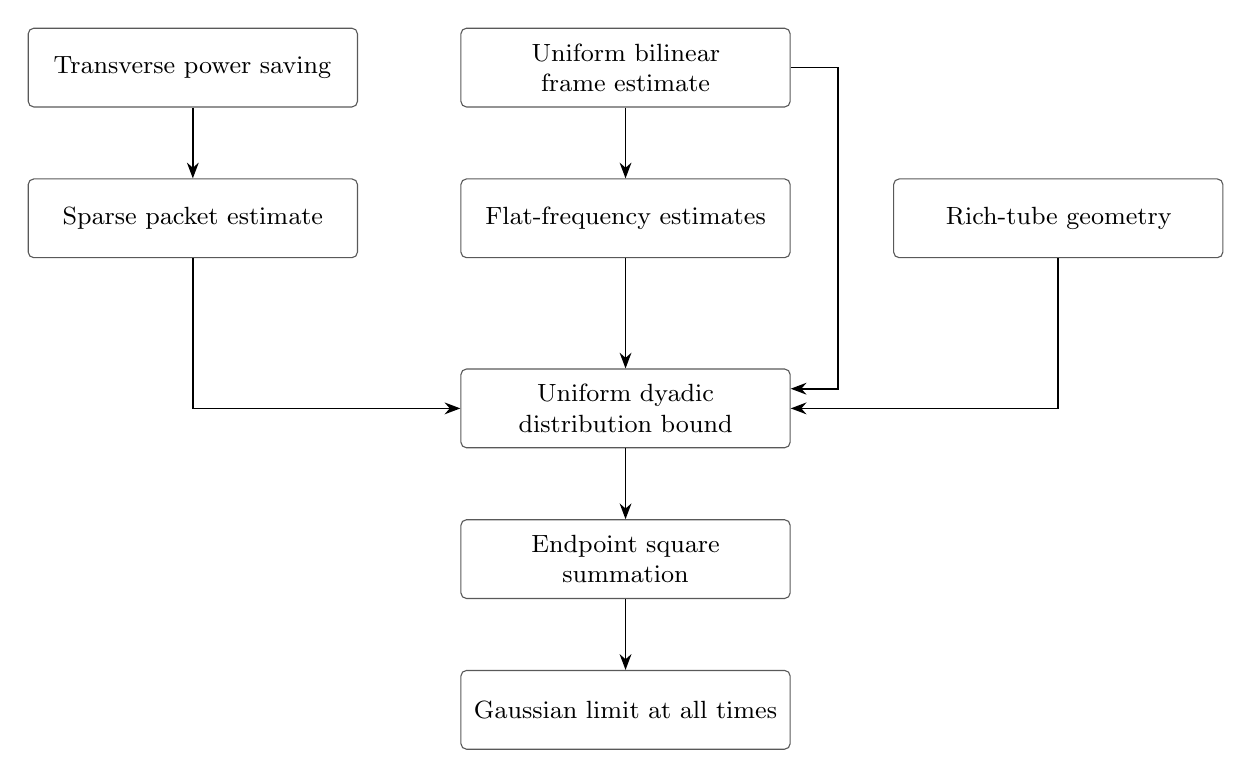
\begin{tikzpicture}[
 node distance=9mm and 13mm,
 box/.style={draw=black!65,rounded corners=2pt,align=center,
             text width=39mm,minimum height=10mm,font=\small,inner sep=4pt},
 arrow/.style={-{Stealth[length=2mm]},semithick}]
 \node[box] (trans) {Transverse power saving};
 \node[box,below=of trans] (sparse) {Sparse packet estimate};
 \node[box,right=of trans] (frame) {Uniform bilinear frame estimate};
 \node[box,below=of frame] (flat) {Flat-frequency estimates};
 \node[box,right=of flat] (geom) {Rich-tube geometry};
 \node[box,below=14mm of flat] (dist) {Uniform dyadic\\distribution bound};
 \node[box,below=of dist] (sum) {Endpoint square summation};
 \node[box,below=of sum] (limit) {Gaussian limit at all times};
 \draw[arrow] (trans)--(sparse);
 \draw[arrow] (frame)--(flat);
 \draw[arrow] (frame.east) -- ++(6mm,0) |- ([yshift=2.5mm]dist.east);
 \draw[arrow] (sparse.south)|-(dist.west);
 \draw[arrow] (flat)--(dist);
 \draw[arrow] (geom.south)|-(dist.east);
 \draw[arrow] (dist)--(sum);
 \draw[arrow] (sum)--(limit);
\end{tikzpicture}
\caption{Dependencies of the proof. Small scale losses are allowed in the
transverse and sparse arguments; the frame and dyadic distribution estimates
must be uniform in the packet scale.}
\label{fig:dependencies}
\end{figure}


\section{Packets, localization, and fractal estimates}
\label{sec:preliminaries}

We first fix the packet conventions and the analytic estimates used in the
transverse argument.  There are two packet classes: compactly supported smooth
atoms, which are convenient for the later geometric arguments, and exact
Schr\"odinger packets, which permit the use of restriction estimates.  The latter
have rapidly decreasing spatial tails.  Keeping these two classes distinct will
also make the localization errors explicit.

\subsection{Conventions and the compact atom class}

For frequency data $v\in L^2(\R^2)$ supported in a fixed bounded set, put
\begin{equation}
 Ev(x,t)=\int_{\R^2}e^{i(x\cdot\xi-t|\xi|^2)}v(\xi)\,d\xi.
 \label{eq:prelim-extension}
\end{equation}
Thus extension input norms are frequency-space $L^2$ norms; the Fourier
normalization in Section~\ref{sec:introduction} differs only by the fixed factor
$(2\pi)^{-2}$.  In particular, with that Fourier convention,
$\|f\|_2^2=(2\pi)^{-2}\|\widehat f\|_2^2$.
All frequency sets below lie in fixed bounded boxes unless another scale is
specified.  The direction associated with $\xi$ is the line parallel to
$(2\xi,1)$, or its unit representative with positive last coordinate.  On a
fixed bounded frequency set, distances between frequencies and between these
unit representatives are comparable.

Unless stated otherwise, all measures are nonnegative Borel measures on space-time $\R^3$.  A ball
bound is required for balls with arbitrary centers.  Its normalizing parameter
may be assumed positive, since the zero case is immediate.  Lattice partitions
are half-open; a supremum on a cell may be taken on its closure.  Fixed
enlargements, boundedly overlapping grids, and fixed changes of frequency boxes
cost constants independent of the large scales and of the number of packets.
All distribution thresholds are positive.

An estimate with a free factor $S^\epsilon$ is asserted for each fixed
$\epsilon>0$, with a constant that may depend on $\epsilon$.  We can therefore
use a smaller exponent to absorb a fixed number of logarithms.  On a
countersequence, $o(1)$ denotes a quantity tending to zero; simultaneous
statements at countably many fixed parameters are obtained by subsequences and
diagonal choices.  Parameters reused in different arguments have only their
local meaning.

\begin{definition}[Compact atoms]
\label{def:prelim-atoms}
Let $L\geq1$, and set $R=L^2$.  An atom with label $\alpha$ is the field
\begin{equation}
 A_\alpha(x,t)=L^{-1}
 e^{i(x\cdot\omega_\alpha-t|\omega_\alpha|^2)}
 H_\alpha\left(\frac{x-b_\alpha-2\omega_\alpha t}{L},
                  \frac{t}{L^2}\right).
 \label{eq:src5}
\end{equation}
The frequencies $\omega_\alpha$ lie in a fixed square.  The labels obey a
joint phase-space bound: every unit ball in $\R^2\times\R^2$ contains at most
a fixed number of the pairs
\[
 \left(\frac{b_\alpha}{L},L\omega_\alpha\right).
\]
The profiles $H_\alpha(y,\tau)$ are supported in a fixed bounded box, and
have uniform bounds for sufficiently many derivatives.  More precisely, each
application requires a finite integer $J$ and fixed bounds
$\|\partial^\beta H_\alpha\|_\infty\leq C_\beta$ for $|\beta|\leq J$.
The integer $J$ is chosen after the fixed parameters of that application; it
does not grow with $L$ or with the array cardinality.  A packet field is a finite
sum $\sum_\alpha c_\alpha A_\alpha$, and its coefficient energy is
$\sum_\alpha|c_\alpha|^2$, without weights.
\end{definition}

The joint phase-space condition does not require bounded multiplicity of
frequencies alone.  In particular, arbitrarily many spatial translates of one
frequency are allowed.  Constants in packet estimates may depend on the fixed
support, multiplicity, and derivative bounds in
Definition~\ref{def:prelim-atoms}.  Whenever a later estimate permits an
arbitrary fixed decay order, sufficiently many of these finitely many
derivatives are to be fixed first.

Suppose that $\mu$ is restricted to $|t|\leq C L^2$ and satisfies
\begin{equation}
 \mu(B(z,r))\leq m r^2 \qquad(z\in\R^3,\ r\geq1).
 \label{eq:prelim-ball-bound}
\end{equation}
The additional sparsity assumption, with the fixed choice $M=100$, is
\begin{equation}
 \int_{\R^3}
 \left(1+\frac{|x-b_\alpha-2\omega_\alpha t|}{L}\right)^{-M}
 \,d\mu(x,t)
 \leq\frac{mL^3}{D}
 \quad\text{for every label used.}
 \label{eq:src6}
\end{equation}
Other sufficiently large fixed values of $M$ would work.  The ball bound alone
implies \eqref{eq:src6} with $D=1$ up to a fixed constant.  Indeed, the
$\rho$-neighborhood of one trajectory on this time slab is covered by
$O(1+L^2/\rho)$ balls of radius $C\rho$.  For $\rho=2^kL$, its mass is at most
\[
 Cm\bigl(2^kL^3+2^{2k}L^2\bigr).
\]
Summing these bounds against $2^{-Mk}$, $k\geq0$, proves the assertion.

The normalization in \eqref{eq:src5} is chosen to be stable under cap
rescaling.  For labels in a square of side $h^{-1}$ centered at $v$, where
$1\leq h\leq L$, set
\begin{equation}
 (x',t')=\left(\frac{x-2vt}{h},\frac{t}{h^2}\right),\qquad
 L'=\frac Lh,\quad b'_\alpha=\frac{b_\alpha}{h},\quad
 \omega'_\alpha=h(\omega_\alpha-v).
 \label{eq:prelim-atom-rescaling}
\end{equation}
An exact substitution gives
\begin{equation}
 A_\alpha(x,t)=h^{-1}e^{i(x\cdot v-t|v|^2)}A'_\alpha(x',t'),
 \label{eq:prelim-atom-covariance}
\end{equation}
where $A'_\alpha$ has the same profile and the parameters in
\eqref{eq:prelim-atom-rescaling}.  The coefficients are unchanged, and
\[
 \left(\frac{b'_\alpha}{L'},L'\omega'_\alpha\right)
 =\left(\frac{b_\alpha}{L},L\omega_\alpha-Lv\right),
\]
so the phase-space ball counts are unchanged as well.  If $\mu'$ is the
pushforward of $\mu$, an inverse image of an $r$-ball is covered by $O(h)$
balls of radius $Chr$.  Hence $\mu'$ has ball parameter $m'=Cmh^3$.
The integrand in \eqref{eq:src6} is invariant under this change, and
$m'(L')^3=CmL^3$, so its sparsity parameter is preserved up to the allowed
fixed constants.  On a time slab of length $O((L')^2)$ centered at zero, a
compact packet meets only $O(1)$ spatial squares of side $(L')^2$.  Thus the
energies assigned to these squares sum with bounded overlap.

\subsection{Exact packets and spatial localization}

The corresponding energy statement for exact fields requires controlling the
tails rather than declaring the packets compactly supported.

\begin{lemma}[Exact packet localization]
\label{lem:packets}
Let $s\geq1$, let $v$ have frequency support in a fixed bounded set, and
consider $|t|\leq Cs^2$.  There is a decomposition
$v=\sum_{\omega,n}a_{\omega,n}v_{\omega,n}$, with
$\omega\in s^{-1}\mathbb{Z}^2$ in a fixed bounded enlargement and
$b_n=sn$, $n\in\mathbb{Z}^2$, such that
\begin{align}
 \sum_{\omega,n}|a_{\omega,n}|^2&\leq C\|v\|_2^2,
 \label{eq:prelim-packet-energy}\\
 \left\|\sum_{(\omega,n)\in\mathcal I}
                  a_{\omega,n}v_{\omega,n}\right\|_2^2
 &\leq C\sum_{(\omega,n)\in\mathcal I}|a_{\omega,n}|^2
 \quad\text{for every subfamily }\mathcal I,
 \label{eq:prelim-subseries-energy}\\
 |Ev_{\omega,n}(x,t)|&\leq C_Ns^{-1}
 \left(1+\frac{|x-b_n-2t\omega|}{s}\right)^{-N}
 \quad(N\geq1).
 \label{eq:prelim-packet-decay}
\end{align}
The constants are independent of the number of terms retained.  The
phase-space label counts are bounded, and every packet has frequency support
in an $O(s^{-1})$ neighborhood of $\omega$.

Fix $0<\eta<1$.  On a set $\Omega$ in this time slab, retain the packets
whose trajectories come within $s^{1+\eta}$ of $\Omega$ at the same time.
For every $A>0$, the sum of the omitted packets is bounded pointwise on
$\Omega$ by $C_{A,\eta}s^{-A}\|v\|_2$.
For a partition into spatial squares of side $s^2$, extended over the common
time slab, the retained data $v_Q$ can consequently be chosen so that
\begin{equation}
 \sum_Q\|v_Q\|_2^2\leq C\|v\|_2^2,
 \qquad
 |Ev-Ev_Q|\leq C_{A,\eta}s^{-A}\|v\|_2
 \quad\text{on }Q\times[-Cs^2,Cs^2].
 \label{eq:prelim-box-localization}
\end{equation}
The same conclusions hold on translated time slabs after modulating the
initial datum and writing the trajectories in the recentered time $t-t_0$.
\end{lemma}

\begin{proof}
Take a smooth bounded-overlap partition $\{\chi_\omega\}$ of frequency
space at resolution $s^{-1}$.  We can arrange that
$\chi_\omega(\omega+\eta/s)$ is supported in $[-1,1]^2$.  Put
\[
 g_\omega(\eta)=s^{-1}(\chi_\omega v)(\omega+\eta/s).
\]
Then $\|g_\omega\|_2=\|\chi_\omega v\|_2$.  On
$[-\pi,\pi]^2$, expand $g_\omega$ in the orthonormal Fourier basis:
\[
 g_\omega(\eta)=\sum_{n\in\mathbb{Z}^2}
 a_{\omega,n}(2\pi)^{-1}e^{-in\cdot\eta}.
\]
Choose one smooth cutoff $\psi$ supported in $(-\pi,\pi)^2$ and equal to
one on $[-1,1]^2$.  Multiplying the series by $\psi$ leaves $g_\omega$
unchanged, and gives the packet data
\[
 v_{\omega,n}(\xi)=\frac{s}{2\pi}
 \psi\bigl(s(\xi-\omega)\bigr)
 e^{-isn\cdot(\xi-\omega)}.
\]
Parseval, followed by the bounded overlap of the frequency partition, gives
\eqref{eq:prelim-packet-energy}.  Multiplication by $\psi$ is bounded on
$L^2$, and its translated frequency supports have bounded overlap.  Applying
these two facts to any selected Fourier coefficients proves
\eqref{eq:prelim-subseries-energy}.  This also proves convergence of the
decomposition in $L^2$.  Since all frequency supports remain in a fixed bounded
set, the corresponding extensions converge uniformly in $(x,t)$.

Changing variables $\xi=\omega+\eta/s$ gives
\begin{equation}
 Ev_{\omega,n}(x,t)=\frac{s^{-1}}{2\pi}
 e^{i(x\cdot\omega-t|\omega|^2)}
 \int \psi(\eta)
 e^{i((x-sn-2t\omega)/s)\cdot\eta-i(t/s^2)|\eta|^2}\,d\eta.
 \label{eq:prelim-exact-profile}
\end{equation}
For $|t|/s^2\leq C$, all derivatives of
$\psi(\eta)e^{-i(t/s^2)|\eta|^2}$ are bounded.  Repeated integration by
parts proves \eqref{eq:prelim-packet-decay}.  In particular the profile in
\eqref{eq:prelim-exact-profile} is Schwartz in its first argument, uniformly
on the prescribed time interval.

For clarity, the tail bound is uniform even for infinite packet expansions.
At a fixed point, there are $O(s^2)$ frequency centers.  For each one the
normalized spatial labels form a translate of $\mathbb{Z}^2$, and, for $N>1$,
\[
 \sum_{n:\ |x-sn-2t\omega|>s^{1+\eta}}
 \left(1+\frac{|x-sn-2t\omega|}{s}\right)^{-2N}
 \leq C_Ns^{-\eta(2N-2)}.
\]
The factor $s^{-2}$ from the squared packet bound cancels the
$O(s^2)$ frequency count.  Cauchy--Schwarz and
\eqref{eq:prelim-packet-energy} therefore bound the discarded field by
$C_Ns^{-\eta(N-1)}\|v\|_2$.  Choose $N$ sufficiently large in terms of
$A$ and $\eta$.

Finally, a bounded-velocity trajectory traverses distance $O(s^2)$ in the
time slab.  Since $s^{1+\eta}\leq s^2$, its padded trajectory meets only
$O(1)$ squares of side $s^2$.  Each coefficient is consequently assigned to
only $O(1)$ of the subfamilies defining $v_Q$.
Equation~\eqref{eq:prelim-subseries-energy} proves their summed energy
bound, and the preceding tail estimate proves the second part of
\eqref{eq:prelim-box-localization}.  To center the time interval at $t_0$,
replace $v(\xi)$ by $e^{-it_0|\xi|^2}v(\xi)$ before decomposing it.
\end{proof}

In applications involving polynomially many boxes or a measure of polynomial
total mass, the exponent $A$ is chosen large enough that all these tail errors
remain smaller than any prescribed negative power.  If only a subpower
padding is desired on a countersequence, first fix a positive padding exponent
for each required estimate and then let it decrease through a diagonal choice.
This does not assert a uniform tail constant as $\eta\downarrow0$.

\subsection{The refined fractal estimate and unit-cube suprema}

We use the following specialization of the refined fractal estimate of
Du--Zhang.  We include the reductions from its uniform occupancy formulation,
since both the weights and the suprema will matter later.

\begin{lemma}[Refined fractal estimate]
\label{lem:fractal}
Let $S\geq1$.  Let $\mathcal Q$ be a collection of distinct unit lattice
cubes in a ball of radius $CS$ in $\R^3$.  Suppose that
\begin{equation}
 \#\{Q\in\mathcal Q:Q\cap B(z,r)\ne\varnothing\}
 \leq\gamma r^2\quad(1\leq r\leq CS),
 \qquad
 \#\{Q\in\mathcal Q:Q\cap B(z,\sqrt S)\ne\varnothing\}
 \leq\lambda_0
 \label{eq:prelim-fractal-counts}
\end{equation}
for all centers $z$, with fixed enlargements of the radius range allowed.
If $v$ has frequency support in a fixed bounded set, then
\begin{align}
 \int_{\bigcup\mathcal Q}|Ev|^2\,dx\,dt
 &\leq C_\epsilon S^\epsilon
       (\gamma\lambda_0S)^{1/3}\|v\|_2^2,
 \label{eq:prelim-fractal-integral}\\
 \sum_{Q\in\mathcal Q}\sup_Q|Ev|^2
 &\leq C_\epsilon S^\epsilon
       (\gamma\lambda_0S)^{1/3}\|v\|_2^2.
 \label{eq:prelim-fractal-sup}
\end{align}
These estimates are uniform under translations of the collection of cubes.
\end{lemma}

\begin{proof}
For unit-ball frequency support, Theorem~1.6 of \cite{DZ19}, specialized to
spatial dimension $2$ and counting exponent $2$, gives
\[
 \|Ev\|_{L^2(X)}
 \leq C_\epsilon S^\epsilon
       \gamma^{1/6}\lambda^{1/6}S^{1/6}\|v\|_2
\]
when every occupied square-root-scale lattice cube contains a comparable
number $\lambda$ of the unit cubes of $X$.  Its time sign is changed by
reflection, and its physical-space input norm is converted to the
frequency-space norm by Plancherel.  A bounded frequency enlargement is
reduced to unit frequency by a fixed parabolic dilation and bounded cube
coverings.  None of these operations changes a large-scale exponent.

For the asserted upper occupancy version, take an ambient radius comparable
to $S$ whose square root is an integer, large enough to contain the given
ball.  Its square-root grid then contains whole unit lattice cubes.  The
occupancy of each parent is at most $C\lambda_0$, since such a parent is
covered by a fixed number of $\sqrt S$-balls.  Sort the parents by their
dyadic occupancy $\lambda$.  Every resulting union retains the counting
bound $C\gamma r^2$.  Apply the quoted theorem to each union, square it,
and sum.  The geometric sum of $\lambda^{1/3}$ is at most
$C\lambda_0^{1/3}$; using a logarithmic bound would also suffice after
decreasing the chosen small exponent.  Renaming that exponent proves
\eqref{eq:prelim-fractal-integral}.  Ball centers can be translated at the
cost of replacing $v(\xi)$ by
$e^{i(y\cdot\xi-u|\xi|^2)}v(\xi)$, which preserves its norm and support.

To obtain suprema, let $F=Ev$.  Its space-time Fourier transform is supported
on a fixed compact portion of the paraboloid.  Choose a Schwartz function
$\rho$ whose Fourier transform is one on that compact set, so that
$F=F*\rho$.  For every unit cube $Q$ and every $z\in Q$,
\begin{equation}
 \sup_{y\in Q}|F(y)|
 \leq C_N\int_{\R^3}(1+|w|)^{-N}|F(z+w)|\,dw.
 \label{eq:prelim-reproducing}
\end{equation}
Indeed, taking the supremum over $y-z$ in a fixed bounded set in the
convolution formula leaves a rapidly decreasing majorant for the kernel.
Cauchy--Schwarz with this integrable weight, followed by integration over
$z\in Q$ and summation in $Q$, gives
\[
 \sum_{Q\in\mathcal Q}\sup_Q|F|^2
 \leq C_N\int_{\R^3}(1+|w|)^{-N}
       \int_{\bigcup\mathcal Q}|Ev(z+w)|^2\,dz\,dw.
\]
For each fixed $w=(y,u)$ the inner field is the extension of the modulated
datum above.  Apply \eqref{eq:prelim-fractal-integral} on the unchanged
domain and integrate the weight.  This proves
\eqref{eq:prelim-fractal-sup} without enlarging the ambient scale according
to the translation.
\end{proof}

The same reproducing argument applies separately to factors in a product.
For example, if $F_i=Ev_i$, $i=1,2,3$, then
\begin{equation}
 \sum_{Q\in\mathcal Q}\prod_{i=1}^3\sup_Q|F_i|
 \leq C_N\int_{(\R^3)^3}\prod_{i=1}^3(1+|w_i|)^{-N}
 \int_{\bigcup\mathcal Q}\prod_{i=1}^3|Ev_i(z+w_i)|\,dz
 \,dw_1\,dw_2\,dw_3.
 \label{eq:prelim-product-suprema}
\end{equation}
To see this, multiply \eqref{eq:prelim-reproducing} for the three fields,
integrate over each unit cube, and use Tonelli.  For each fixed triple of
shifts, the three exact fields are tested at the same integration point on
the same domain.  Their data have independent unimodular modulations, which
preserve supports, norms, and frequency transversality.  This is the version
used when applying multilinear restriction to products of cube suprema.

\subsection{Weights and cap rescaling}

\begin{lemma}[Weighted refined estimate]
\label{lem:prelim-weighted}
Let $\nu$ be supported in a ball of radius $CS$, $S\geq1$, and suppose
\begin{equation}
 \nu(B(z,r))\leq mr^2\quad(r\geq1),\qquad
 \nu(B(z,\sqrt S))\leq mSd
 \quad(z\in\supp\nu),
 \label{eq:prelim-weighted-hypotheses}
\end{equation}
where $m,d>0$.  For bounded frequency support,
\begin{equation}
 \int |Ev|^2\,d\nu
 \leq C_\epsilon S^\epsilon mS^{2/3}d^{1/3}\|v\|_2^2.
 \label{eq:prelim-weighted-fractal}
\end{equation}
The same bound holds for
$\sum_Q\nu(Q)\sup_Q|Ev|^2$, summed over unit cubes.  The ball bound alone
gives this conclusion with $d=1$, up to a fixed constant.
\end{lemma}

\begin{proof}
Fixed-radius enlargements of the second bound in
\eqref{eq:prelim-weighted-hypotheses} follow by a bounded covering with
balls of radius $\sqrt S$ centered on the support.  This also extends it
to arbitrary centers, up to a fixed constant.  Every unit cube has mass
at most $Cm$.  Split the positive-mass cubes into classes
\[
 m\chi<\nu(Q)\leq2m\chi,
 \qquad \chi\in\{C_02^{-k}:k\geq0\},
\]
with harmless endpoint adjustments and fixed $C_0$.  Cubes in one class
have counting parameter $C\chi^{-1}$: the cubes meeting an $r$-ball have
disjoint masses inside a fixed enlargement of that ball.  Their
square-root-scale occupancy is at most $CSd\chi^{-1}$ by the same
argument.  Lemma~\ref{lem:fractal} therefore gives
\begin{align*}
 \sum_{Q\text{ in the }\chi\text{ class}}\nu(Q)\sup_Q|Ev|^2
 &\leq C_\epsilon m\chi S^\epsilon
   \bigl(\chi^{-1}\cdot Sd\chi^{-1}\cdot S\bigr)^{1/3}
   \|v\|_2^2\\
 &=C_\epsilon S^\epsilon mS^{2/3}d^{1/3}
   \chi^{1/3}\|v\|_2^2.
\end{align*}
The series $\sum_\chi\chi^{1/3}$ converges.  Summing proves both
assertions, including measures with arbitrarily small positive cube masses;
no lower mass cutoff is needed here.  Finally the first ball bound, evaluated
at $r=\sqrt S$, supplies $d=1$.
\end{proof}

\begin{lemma}[Weighted cap estimate]
\label{lem:cap}
Fix $\alpha_0<1/2$.  Suppose that $S\geq1$, that $\nu$ is supported in
a ball of radius $CS$ and satisfies $\nu(B(z,r))\leq mr^2$ for $r\geq1$,
and that $v$ is supported in a frequency ball $B(v_0,q)$, with $v_0$ in a
fixed bounded set and
\[
 S^{-\alpha_0}\leq q\leq1.
\]
Then, for every $\epsilon>0$,
\begin{equation}
 \int |Ev|^2\,d\nu
 \leq C_{\epsilon,\alpha_0}S^\epsilon
       mS^{2/3}q^{1/3}\|v\|_2^2.
 \label{eq:prelim-cap-estimate}
\end{equation}
The estimate also holds with the integral replaced by
$\sum_Q\nu(Q)\sup_Q|Ev|^2$ over unit cubes.  Bounded translations, and
averages of translations with a fixed integrable Schwartz weight, obey the
same bounds.
\end{lemma}

\begin{proof}
Translate the space-time support ball to the origin, absorbing the
translation in a unimodular factor on $v$.  Write
\[
 g(\eta)=q\,v(v_0+q\eta),\qquad
 (y,\tau)=\bigl(q(x-2v_0t),q^2t\bigr),\qquad S'=Sq^2.
\]
Then $\|g\|_2=\|v\|_2$, $\supp g\subset B(0,1)$, and
\begin{equation}
 Ev(x,t)=q\,e^{i(x\cdot v_0-t|v_0|^2)}Eg(y,\tau).
 \label{eq:prelim-cap-identity}
\end{equation}
Let $\nu'$ be the pushforward of $\nu$.  The inverse map is
\[
 t=q^{-2}\tau,\qquad x=q^{-1}y+2v_0q^{-2}\tau.
\]
Consequently, the inverse image of a ball of radius $r\geq1$ is a bounded
shear of a box with side lengths $r/q,r/q,r/q^2$.  It is covered by
$O(q^{-1})$ balls of radius $Cr/q$.  The original ball bound applies at
these radii and gives
\begin{equation}
 \nu'(B(z,r))\leq Cm q^{-3}r^2\qquad(r\geq1).
 \label{eq:prelim-rescaled-density}
\end{equation}
There is no Jacobian multiplier on this pushforward measure.

The rescaled time interval has length $O(S')$, but the spatial projection
has diameter $O(Sq)=O(S'/q)$.  Partition the latter into squares $Q$ of
side $S'$.  On the common time slab, use Lemma~\ref{lem:packets} at packet
width $s=\sqrt{S'}$, with any fixed padding exponent in $(0,1)$.  Let
$g_Q$ denote its localized data.  Then
\[
 \sum_Q\|g_Q\|_2^2\leq C\|g\|_2^2,
 \qquad |Eg-Eg_Q|\leq C_A(S')^{-A}\|g\|_2
 \quad\text{on the corresponding prism},
\]
where $A$ can be made arbitrarily large.  Each restricted measure lies in a
ball of radius $CS'$, so Lemma~\ref{lem:prelim-weighted} with $d=1$ and
\eqref{eq:prelim-rescaled-density} gives
\[
 \sum_Q\int_{Q\times[-CS',CS']}|Eg_Q|^2\,d\nu'
 \leq C_\epsilon(S')^\epsilon m q^{-3}(S')^{2/3}\|g\|_2^2.
\]
The sum uses the localized energies, rather than the number of spatial
squares.  This distinction is essential for the cap power.

For completeness, $\nu'(\R^3)=\nu(\R^3)\leq CmS^2$, whereas
$S'\geq S^{1-2\alpha_0}$.  Thus the integrated squared error, after
multiplication by the $q^2$ in \eqref{eq:prelim-cap-identity}, is at most
\[
 C_A m q^2 S^2(S')^{-2A}\|g\|_2^2.
\]
Choose $A$ in terms of $\alpha_0$ so that this is bounded by the desired
right side; bounded $S$ is absorbed in the constant.  For the principal term,
\begin{equation}
 q^2\,m q^{-3}(Sq^2)^{2/3}
 =mS^{2/3}q^{1/3}.
 \label{eq:prelim-cap-power}
\end{equation}
Since $(S')^\epsilon\leq S^\epsilon$, this proves
\eqref{eq:prelim-cap-estimate}.

Finally, square \eqref{eq:prelim-reproducing} by weighted
Cauchy--Schwarz, integrate in $z\in Q$ against $d\nu(z)$, and sum the
original unit cubes.  This bounds the sum of weighted suprema by
\[
 C_N\int_{\R^3}(1+|w|)^{-N}
           \int_{\R^3}|Ev(z+w)|^2\,d\nu(z)\,dw.
\]
For every shift the field is an exact extension of modulated data with the
same cap support and norm.  Apply the already proved cap estimate and
integrate the rapidly decreasing weight.  This proves the supremum
assertion and the asserted translated versions.
\end{proof}

\begin{remark}[Enlarged cubes in the inductive formulation]
\label{rem:prelim-enlarged-cubes}
The proof of Lemma~\ref{lem:fractal} is sufficient for all later applications.  For comparison,
we record an alternative reduction of \eqref{eq:prelim-fractal-integral} to
the inductive Proposition~3.1 of \cite{DZ19}.  Choose $K=S^\delta$ with $0<\delta<1/4$ sufficiently small
relative to the desired loss, and enlarge occupied unit cubes to occupied
$K^2$-cubes.  Selecting one original unit cube in each occupied large cube
shows, by ball covering, that the large cubes have counting parameter
$O(\gamma)$ for $r\geq K^2$, and square-root-scale occupancy
$O(\lambda_0)$.  Normalize $\|v\|_2=1$ and discard large cubes with
$L^6$ norm below $S^{-A}$.  There are polynomially many cubes, so their
total $L^2$ contribution is arbitrarily small when $A$ is sufficiently
large.  The remaining $L^6$ norms have only $O(\log S)$ dyadic classes,
since $|Ev|\leq C$ and each large cube has volume $K^6$.

After fixing a norm class, recompute its parent occupancies and sort them
dyadically.  On each resulting union $Y$ of $M_Y$ large cubes,
Proposition~3.1 gives
\[
 \|Ev\|_{L^6(Y)}
 \leq C_\epsilon M_Y^{-1/3}
       (\gamma\lambda_0S)^{1/6}S^\epsilon\|v\|_2.
\]
H\"older contributes
$|Y|^{1/3}=M_Y^{1/3}K^2$ on passing to $L^2$, cancelling $M_Y^{-1/3}$.
After squaring, the additional loss is $K^4$; the finitely many logarithmic
losses and this factor are absorbed by the choice of $\delta$ and a smaller
initial $\epsilon$.

The grids in this deduction can be made compatible as follows.  Increase
the ambient scale by a bounded factor so that
$S^{1/2}/S^{2\delta}$ is an integer.  Such scales have successive ratios
tending to one.  Use nested grids at these two scales and a bounded family
of translated parent grids.  For sufficiently large $S$, each original
unit cube can be assigned to a parent grid in which it is farther than
$2\sqrt3 K^2$ from the parent boundary; keep only the occupied large cubes
within that parent.  Split the original collection according to these
finitely many assignments.  The same original ball counts control each
part, while translation is absorbed into the datum as in
Lemma~\ref{lem:fractal}.  Bounded scales are covered by a fixed constant.
Thus neither boundary cubes nor rounding changes the resulting estimate.
\end{remark}

\section{A power saving for transverse inputs}
\label{sec:transverse}

The first step is a rigidity statement for almost extremizers of the
fractal estimate.  A hypothetical extremizing configuration produces a
probability distribution on points and incident tubes.  Information at
successive spatial scales first forces three identical one-dimensional
profiles, then forces those profiles to alternate only finitely often
between slopes zero and one.  Polynomial partitioning rules out the
remaining transition.

\begin{proposition}[Transverse power saving]\label{prop:transverse}
Fix a bounded frequency region.  There are $c>0$ and $L_0<\infty$,
depending only on that region, for which the following configuration
cannot exist when $L\ge L_0$.  Let $\mathcal Q$ be unit lattice cubes
inside a ball of radius $L^2$ in $\R^3$, with
\[
 \#\mathcal Q\ge L^{4-c},\qquad
 \#\{Q\in\mathcal Q:Q\cap B(z,r)\ne\varnothing\}
       \le L^c r^2\quad(r\ge1),
\]
where cube counts may equivalently use their centers, up to fixed
constants.  Suppose $v_1,v_2,v_3$ have frequency support in the
fixed region, $\|v_i\|_2\le1$, and
\[
 \sup_Q|Ev_i|\ge L^{-4/3-c}
 \qquad(Q\in\mathcal Q,\ i=1,2,3).
\]
Then it is impossible that every triple of unit frequency directions,
one from each support, has absolute determinant at least $L^{-c}$.
\end{proposition}

We argue by contradiction along $L\to\infty$ and $c\downarrow0$.
Every $o(1)$ in this section refers to this sequence or a subsequence.
A diagonal choice converts estimates valid with every fixed positive
power loss into $L^{o(1)}$ estimates; constants are fixed before making
that choice.  All rounding, support enlargements, and packet padding
are included in these subpower errors.  The same convention applies
when a scale is a fixed positive power of $L$.

\subsection{Uniform multilinear estimates and the tube model}

We need the multilinear estimates when transversality itself deteriorates
by a subpower.  An unspecified transversality-dependent constant in the
restriction theorem would not justify this use.  The following finite
induction supplies the required uniformity.

\begin{lemma}[Multilinear estimates with subpower transversality]
\label{lem:transverse-product}
Suppose three exact extension inputs have bounded frequency supports,
and every triple of their unit directions has determinant at least
$\nu$, where $0<\nu\le1$.  For each $\epsilon>0$ there are $C_\epsilon,M_\epsilon<\infty$
such that, on every ball of radius $S\ge2$,
\begin{equation}\label{eq:transverse-product}
 \int_{B_S}\prod_{i=1}^3|Ev_i(z)|\,dz
 \le C_\epsilon\nu^{-M_\epsilon}S^\epsilon
                         \prod_{i=1}^3\|v_i\|_2.
\end{equation}
The same conclusion holds for the sum over unit lattice cubes in the
ball of $\prod_i\sup_Q|Ev_i|$.  In particular, when $\nu=S^{-o(1)}$
both bounds are $S^{o(1)}\prod_i\|v_i\|_2$.
For weighted tubes of width $\Delta$ in a bounded region, the
corresponding multilinear Kakeya bound is
\begin{equation}\label{eq:transverse-kakeya}
 \int\prod_{i=1}^3
       \left(\sum_T w_i(T)\mathbf1_T\right)^{1/2}
 \le C_\epsilon\nu^{-M_\epsilon}\Delta^{3-\epsilon}
                  \prod_{i=1}^3\left(\sum_Tw_i(T)\right)^{1/2}.
\end{equation}
Here fixed enlargements of tubes and of the ambient region are allowed;
if those enlargements are subpower on a sequence, they cost a subpower.
\end{lemma}

\begin{proof}
Partition each direction support into neighborhoods of radius a sufficiently
small fixed power of $\nu$.  There are at most $\nu^{-O(1)}$ such
neighborhoods.  For each triple choose representative directions and send
them to the coordinate axes by a linear map.  Its norm, inverse norm,
and volume distortion are bounded by fixed powers of $\nu^{-1}$.
The transformed direction neighborhoods lie in fixed small neighborhoods
of the axes.  The weighted multilinear Kakeya inequality of
\cite[Theorem~1.15 and Remark~1.10]{BCT06}, applied there and summed over triples, proves
\eqref{eq:transverse-kakeya}.  Weights follow first by repetitions and
then by approximation.  Widths larger than a fixed constant can instead
be treated by the trivial bound, after increasing the inverse-power
constant.

For completeness, use this Kakeya inequality to obtain restriction
uniformity.  Let $A_B(S,\nu)$ be the least normalized product-integral
constant for inputs supported in $[-B,B]^2$.  Fix padding exponent
$\theta>0$ and Kakeya loss $\sigma>0$.  Cover a ball of radius $S$
by cubes of side comparable to $\sqrt S$.  The exact packet
decomposition restricts each input on a smaller cube to packets
incident to its $S^\theta\sqrt S$ enlargement.  Its retained exact
input has squared norm at most a fixed constant times the incident
coefficient energy.  Its support is within $O_B(S^{-1/2})$ of the
original support: only caps intersecting that support occur, and
every enlarged cap lies within this distance of such an intersection.
Thus determinant continuity preserves $\nu/2$ transversality when
$S^{-1/2}\le c_B\nu$, without any openness or connectedness
assumption on the supports.

Apply the smaller-scale product estimate in every cube.  Its geometric
coefficient is the product of the three square roots of incident
energies.  After division of coordinates by $S$, the padded tubes
have width $\Delta=S^{-1/2+\theta}$.  Enlarge them by a fixed factor,
so an incident tube contains the whole smaller grid cube.
Equation~\eqref{eq:transverse-kakeya}, divided by that cube's volume
$S^{-3/2}$, gives the bound
\[
 C_{B,\theta,\sigma}\nu^{-M_\sigma}
 S^{3/2}(S^{-1/2+\theta})^{3-\sigma}
 \prod_i\|v_i\|_2
 \le C_{B,\theta,\sigma}\nu^{-M_\sigma}
 S^\beta\prod_i\|v_i\|_2,\qquad
 \beta=3\theta+\sigma/2,
\]
for the sum of these geometric coefficients.
To bound discarded-field errors, normalize each parent input, use
rapid tails for a discarded factor and the fixed-frequency
$L^\infty$ bound for the others, and expand the three-factor product.
The seven error terms together contribute at most
$C_{B,\theta,N}S^{3-N}\prod_i\|v_i\|_2$, for every prescribed $N$.
This is relative to the current \emph{parent} norms; no lower bound
for a retained local norm is required.  We obtain the recurrence
\begin{equation}\label{eq:transverse-square-root}
 A_B(S,\nu)\le C_{B,\theta,\sigma}\nu^{-M_\sigma}S^\beta
       A_{B+1}(C_B\sqrt S,\nu/2)
       +C_{B,\theta,N}S^{3-N},
 \qquad S^{-1/2}\le c_B\nu.
\end{equation}
Spatial translations only modulate the exact inputs.  Taking $N>3$
and setting $\widetilde A_B=1+A_B$ absorbs the additive error in
the same multiplicative recurrence for $\widetilde A_B$.

Fix the target $\epsilon>0$.  Choose a finite $J$ with
$3\cdot2^{-J}<\epsilon/2$, then choose $\theta,\sigma$ with
$2\beta<\epsilon/2$.  The finitely many radii defined by
$S_0=S$, $S_{j+1}=C_{B+j}\sqrt{S_j}$ are comparable to
$S^{2^{-j}}$, with constants depending only on $B,J$.
If $S\ge(C_{B,J}/\nu)^{2^J}$ for a sufficiently large constant,
all $J$ support-enlargement conditions hold.  Iterating
\eqref{eq:transverse-square-root} and using the terminal trivial
bound $\widetilde A_{B+J}(R,\nu')\lesssim_{B,J}R^3$ gives
\[
 \widetilde A_B(S,\nu)
 \le C_{B,\epsilon}\nu^{-M_{B,\epsilon}}
 S^{\beta\sum_{j=0}^{J-1}2^{-j}+3\cdot2^{-J}}
 \le C_{B,\epsilon}\nu^{-M_{B,\epsilon}}S^\epsilon.
\]
In the complementary range, the trivial bound $A_B(S,\nu)\lesssim_B
S^3$ is absorbed by increasing the fixed inverse-transversality
exponent to at least $3\cdot2^J$.  This proves
\eqref{eq:transverse-product} for all $S,\nu$.  On a subpower-transverse
sequence the threshold is eventually satisfied for each fixed $J$,
and every intermediate enlarged support remains subpower transverse.
This is a finite version of the restriction bootstrapping in
\cite[Proposition~2.1]{BCT06}; polynomial dependence is supplied by this argument,
not by the statement of their restriction theorem alone.

Finally, fixed-frequency reproducing kernels give, for $z\in Q$,
\[
 \sup_Q|Ev_i|\lesssim_N
       \int(1+|w|)^{-N}|Ev_i(z+w)|\,dw.
\]
Integrate the product over $Q$ and sum.  For each triple of shifts the
three shifted fields are exact extensions on the same domain, with
independently modulated inputs of unchanged norms and supports.  Apply
\eqref{eq:transverse-product} and integrate the Schwartz weights.
\end{proof}

\begin{lemma}[Reduction to weighted incident tubes]
\label{lem:transverse-tubes}
A countersequence to Proposition~\ref{prop:transverse} yields a set
$P$ in a fixed bounded region and three weighted tube families satisfying
\begin{equation}\label{eq:transverse-point-counts}
 |P|=L^{2+o(1)},\qquad
 |P\cap B(z,r)|\le L^{2+o(1)}r^2
             \quad(L^{-1}\le r\le1).
\end{equation}
The points are centers of distinct cubes of side comparable to $L^{-1}$.
The tubes have width $L^{-1+o(1)}$, their coefficient weights obey
$\sum_Tw_i(T)\lesssim1$, and every cross-family direction triple has
determinant at least $L^{-o(1)}$.  At each $p\in P$ there is a retained
incident subfamily of total weight $e_i^*(p)=L^{-4/3+o(1)}$ such that
its normalized weight law satisfies, for fixed $\kappa>0$, $u_0>0$,
\begin{equation}\label{eq:src1}
 \Prob\bigl(\operatorname{dir}T_i\in B(v,L^{-u})\mid X=p\bigr)
       \le L^{-\kappa u+o(1)}
       \qquad(0<u<u_0,\ u\in\mathbb Q).
\end{equation}
This bound is uniform in $p,v$ for each fixed rational $u$.
The retained subfamily may depend on $p$.
\end{lemma}

\begin{proof}
Sort occupied $L$-boxes by their number of selected unit cubes.
A dyadic occupancy class retains $L^{4-o(1)}$ cubes.  The squared
supremum sum for each field on this class is at least
$L^{4/3-o(1)}$.  By Lemma~\ref{lem:fractal} at radius $L^2$, a class
with occupancy at most $L^{2-\delta}$, for fixed $\delta>0$, instead
has squared sum at most $L^{4/3-\delta/3+o(1)}$.  Thus some retained
class has $L^{2-o(1)}$ cubes in each occupied box.  The upper counting
bound gives occupancy at most $L^{2+o(1)}$.  Divide coordinates by
$L^2$ and take the centers of these boxes.  Counting cubes in an
enlarged ball and dividing by the minimum occupancy proves
\eqref{eq:transverse-point-counts}.  Translation of the original
ambient ball merely modulates the exact data.

Apply Lemma~\ref{lem:packets} at packet width $L$ on the time
interval of length $O(L^2)$.  After division of coordinates by $L^2$,
the resulting tubes have width $L^{-1+o(1)}$.  Give each tube the
squared coefficient of its packet as weight.  On each retained box,
packets reaching a padded enlargement give an exact local input and
an error $O(L^{-100})$.  The padding exponent tends sufficiently
slowly to zero; the rapid-tail estimates permit this by diagonalization.
By \eqref{eq:prelim-subseries-energy}, the squared norm of this
exact local input is bounded by the incident coefficient energy
$e_i(p)=\sum_{T\ni p}w_i(T)$ up to a constant.  On the at least
$L^{2-o(1)}$ selected unit cubes in this box the required squared
supremum sum is $L^{-2/3-o(1)}$.  The weighted fractal estimate at
radius $L$ bounds it above by $L^{2/3+o(1)}e_i(p)$, so
\[
 e_i(p)\ge L^{-4/3-o(1)}.
\]
Lemma~\ref{lem:transverse-product}, in its Kakeya form and with
$\Delta=L^{-1+o(1)}$, yields
\[
 \sum_{p\in P}\prod_{i=1}^3e_i(p)^{1/2}\le L^{o(1)}.
\]
For fixed $\delta>0$, points at which some
$e_i(p)\ge L^{-4/3+\delta}$ therefore number at most
$L^{2-\delta/2+o(1)}$.  Discarding these points by a diagonal choice
leaves \eqref{eq:transverse-point-counts} and makes all three energies
$L^{-4/3+o(1)}$ uniformly.

It remains to remove concentration in direction without losing the
local lower bound.  Choose $0<\kappa<1/3$ and $0<u_0<1/4$.
For each fixed rational $0<u<u_0$, put $q=L^{-u}$ and partition
directions into bounded-overlap bins of diameter comparable to $q$.
Delete incident bins having weight greater than $q^\kappa e_i(p)$.
There are $O(q^{-\kappa})$ such bins.  On the original box of radius
$O(L)$, Lemma~\ref{lem:cap} applies with $S=L$; the packet frequency
enlargement $O(L^{-1})$ is smaller than the bin width $q$.
Cauchy--Schwarz over the deleted bins then bounds the squared
supremum sum of their combined field by
\[
 L^{2/3+o(1)}q^{1/3-\kappa}e_i(p).
\]
Here the chosen unit cubes have local density $L^{o(1)}$, and the
energies of all deleted bins sum to $O(e_i(p))$.  The estimate also
holds for arbitrary subfamilies of these bins.  For every fixed $u>0$
this is negligible relative to $L^{-2/3-o(1)}$.

Delete successively for any fixed finite list of rational $u$'s,
assigning a packet deleted more than once to just one bin.  The
triangle inequality in the square-sum norm shows that the surviving
field retains its lower local norm.  The unrestricted local estimate
then gives surviving weight $e_i^*(p)=L^{-4/3+o(1)}$.  Every surviving
bin has original weight at most $q^\kappa e_i(p)$; normalizing by
$e_i^*(p)$ costs only $L^{o(1)}$.  Boundedly many neighboring bins
cover a ball, and a diagonal choice proves \eqref{eq:src1} at all fixed
rational scales.  All estimates were uniform in $p$, so this
point-dependent pruning supplies legitimate conditional laws without
requiring a single globally pruned family.
\end{proof}

\subsection{Information at spatial scales}

From now on only the abstract configuration of
Lemma~\ref{lem:transverse-tubes} is used.  Draw $X$ uniformly from $P$.
Given $X$, draw six tubes $T_i,T_i'$ independently, two from each
retained family.  A tube label includes its exact direction.  For
rational $0<s\le1$, let $X_s$ be the cell containing $X$ in nested
dyadic grids of side comparable to $L^{-s}$; use the trivial partition
at $s=0$.  For a discrete variable $Y$ and arbitrary conditioning $V$,
write
\[
 I_L(Y\mid V)=-\log_L\Prob(Y=Y(\omega)\mid V)
\]
for its information evaluated at the sampled labels.  Conditional
probabilities may be fixed in any version on null sets.
This is the exponent of the reciprocal probability of the realized label,
rather than its expectation: a sampled label of conditional probability
$L^{-a+o(1)}$ has information $a+o(1)$.  We retain these sampled
exponents in one joint limiting law so that comparisons at different
spatial scales refer to the same configuration.

\begin{lemma}[Limiting information calculus]
\label{lem:transverse-information}
After a subsequence, all the countably many information variables used
below have a common limiting joint law.  For spatial, coordinate, and
direction partitions with at most $L^{C+o(1)}$ possible labels,
their conditional informations are uniformly integrable and have
bounded limiting values.  In this law the chain rule remains exact and
\begin{equation}\label{eq:transverse-conditioning}
 I(Y\mid V)\ge I(Y\mid V,W)\quad\hbox{almost surely}.
\end{equation}
If, given $Z,V$, the possible values of $Y$ on an event $E_L$
number at most $L^{\gamma+o(1)}$, include its indicator in the
joint limit.  On the event where the limiting indicator equals one,
$I(Y\mid Z,V)\le\gamma$.  Alternatively, an event specified by
a finite system of sampled inequalities can be treated by open-set
implications with fixed slack before that slack tends to zero; no
identification of arbitrary boundary events is implicit.  Consequently
variables determining one
another up to $L^{o(1)}$ possibilities have identical limiting
information, also after additional conditioning.  Finite systems of
limiting inequalities holding with positive probability pass to
finite $L$ with any fixed positive slack.
\end{lemma}

\begin{proof}
A variable with at most $L^{C+o(1)}$ labels satisfies, uniformly in
conditioning,
\[
 \Prob\{I_L(Y\mid V)>C+\eta\}\le L^{-\eta+o(1)}.
\]
The same counting argument with a varying threshold proves uniform
integrability.  For the conditioning assertion put
$p=\Prob(Y\mid V)$ and $q=\Prob(Y\mid V,W)$ at the sampled labels.
Conditional on $(V,W)$, the expectation of $p/q$ is at most one.
Thus
\[
 \Prob\{I_L(Y\mid V)-I_L(Y\mid V,W)<-\eta\}
       \le L^{-\eta}.
\]
This proves the almost-sure sign in the limit; no finite-scale
pointwise monotonicity is asserted.  The chain rule is pointwise
already at finite scale.  The determination rule follows by summing
over the stated small set of possible labels.  This argument also
works on restricted events, since it bounds the total mass of the
bad low-probability labels in the event's permitted set.  If the
event indicator is included in the joint limit, apply weak convergence
to the open set where it is one and the information is strictly
above $\gamma+\eta$, and then let $\eta\downarrow0$.  For events
defined through other limiting variables, the same argument uses
strict inequalities and slack, as detailed in the zero-ratio
application below.

Tightness and diagonal weak convergence on a countable product give
the joint law.  Include in this product all rational block and prefix
parameters, all finitely many choices of reference and replacement
tubes, their direction bins, coordinate grids, projections, the
information differences used below, and the angular quantities to be
introduced.  Direction grids use deterministic representatives of
occupied bins.  Realized bases and inverse bases have norms
$L^{o(1)}$, so every coordinate partition has at most $L^{C+o(1)}$
labels.  Standard open-set inequalities for weak convergence justify
the assertion about finite systems after enlarging their bounds by
slack.  Uniform integrability permits passage of expectations in the
cost estimates below.
\end{proof}

\begin{lemma}[The spatial profiles]\label{lem:transverse-profiles}
In the limiting law set
\[
 F(s)=I(X_s),\qquad G_i(s)=I(X_s\mid T_i),\qquad
 G_i'(s)=I(X_s\mid T_i').
\]
These functions extend from rational scales to nondecreasing Lipschitz
functions on $[0,1]$, vanishing at zero.  Their Lipschitz constants
are respectively $3$ and $1$.  Almost surely,
\begin{equation}\label{eq:transverse-endpoint-information}
 F(s)\ge2s,\qquad F(1)=2,\qquad
 G_i(1),G_i'(1)\ge\tfrac23.
\end{equation}
\end{lemma}

\begin{proof}
The exact chain increment of $G_i$ between $s$ and $s+t$ is
$I(X_{s+t}\mid X_s,T_i)$.  Inside a parent, the tube meets at most
$L^{t+o(1)}$ child cubes, including its padding.  The determination
rule bounds this increment between zero and $t$; the unrestricted
spatial count gives the bounds zero and $3t$ for $F$.  Rational
comparisons simultaneously yield the Lipschitz extensions.

The ball count in \eqref{eq:transverse-point-counts} gives every
$X_s$-cell mass at most $L^{-2s+o(1)}$, proving $F(s)\ge2s$.
An $X_1$-cell contains boundedly many points and $X$ is uniform, so
$F(1)=2$.  Finally the retained weights give
\[
 \Prob(X=p,T_i=T)
   =|P|^{-1}\frac{w_i(T)\mathbf1_{\{T\text{ retained at }p\}}}
                      {e_i^*(p)}
   \le L^{-2/3+o(1)}w_i(T).
\]
The probability of sampling a tube whose marginal is smaller than
$L^{-\eta}w_i(T)$ is at most
$L^{-\eta}\sum_Tw_i(T)=O(L^{-\eta})$.  Outside this event, every
conditional point mass is at most $L^{-2/3+\eta+o(1)}$.
Letting $\eta\downarrow0$ proves the conditional endpoint bounds,
also for all primed tubes.  This uses only summability of weights,
so exact tube labels need not have bounded cardinality.
\end{proof}

\subsection{Direction costs and equality of the profiles}

To compare the three tube-conditional profiles, we use coordinates
adapted to one reference tube from each family.  Specifying those
coordinates requires revealing coarse direction bins.  This can lower
the spatial information; the costs below measure that loss, and their
telescoping bound will let the loss tend to zero with the block size.

Fix a rational block $[s,s+b]\subset[0,1]$ and rational $b_*\ge b$.
Let $C=X_s$ and let $D$ record direction bins of precision $L^{-b_*}$
for a fixed sublist of the six tubes, including one reference tube
from each family.  Within the parent subtract its center, multiply
coordinates by $L^s$, and use the approximate basis supplied by the
three reference bins.  Its norms and inverse norms are $L^{o(1)}$.
For rational $0<t\le b$ let $Z_i$ be its $i$th coordinate grid index
at resolution $L^{-t}$, and write $Z=(Z_1,Z_2,Z_3)$ and
$Z_{\widehat i}=(Z_j)_{j\ne i}$.  These coordinate grids are nested
in $t$.  When extra bins are added to $D$, the basis is still selected
using only the three reference bins, so the coordinate variables do
not change.

\begin{lemma}[Block comparison and telescoping costs]
\label{lem:transverse-costs}
Write $J=F(s+t)-F(s)$ and $J_i=G_i(s+t)-G_i(s)$ for the chosen
reference tubes.  Define
\[
 \ell=I(X_{s+t}\mid C)-I(X_{s+t}\mid C,D),\qquad
 \ell_i=I(X_{s+t}\mid C,T_i)-I(X_{s+t}\mid C,T_i,D).
\]
All these limiting costs are nonnegative, and
\begin{equation}\label{eq:src2}
 \sum_{i=1}^3(J_i-\ell_i)
 \le\sum_{i=1}^3I(Z_i\mid Z_{\widehat i},C,D)
 \le I(Z\mid C,D)=J-\ell.
\end{equation}
For disjoint blocks or disjoint prefixes, with the same $D$, the
sum of expectations of each type of cost is $O(b_*)$.  The same
statement holds with any one fixed other tube in place of $T_i$.
All coordinatewise deficits obtained by using any ordering in the
second inequality of \eqref{eq:src2} are nonnegative.
\end{lemma}

\begin{proof}
The spatial child and the three coordinate labels determine one
another up to $L^{o(1)}$ choices.  A reference tube determines its
two off-axis coordinates to $L^{o(1)}$ choices: both its width and
the error in its approximate direction, relative to the parent,
are at most $L^{-t+o(1)}$.  Conditional information calculus therefore
gives
\[
 J_i-\ell_i=I(Z_i\mid C,D,T_i)
   =I(Z_i\mid Z_{\widehat i},C,D,T_i)
   \le I(Z_i\mid Z_{\widehat i},C,D).
\]
For each ordering of the coordinates, its chain-rule term conditions
on a subset of $Z_{\widehat i}$, hence dominates the last expression.
Sum the three terms to obtain \eqref{eq:src2}.

At finite scale, the expected cost is the conditional mutual
information, divided by $\log L$, between the child and $D$ given
the parent (and, when present, the same fixed tube).  Along the nested
spatial filtration these mutual informations telescope.  Inserting
the omitted gaps between disjoint blocks only adds nonnegative
expected terms.  Their sum is at most $H(D)/\log L=O(b_*)$, because
there are $L^{O(b_*)}$ direction-bin lists.  Fixed tube conditioning
is never changed within this telescoping argument.  Passage to the
limit follows from Lemma~\ref{lem:transverse-information}.
\end{proof}

\begin{lemma}[Additivity and replacement invariance]
\label{lem:transverse-additivity}
Almost surely, simultaneously for every choice of one of the two
tubes in each family,
\[
 F=G_1+G_2+G_3,\qquad G_i'=G_i,\qquad G_i(1)=\tfrac23.
\]
In any block above, including a prefix and with any extra direction
bins in $D$,
\begin{equation}\label{eq:src3}
 \begin{split}
 I(Z_i\mid C,D)&=J_i+O\left(\sum_k\ell_k\right),\\
 I(Z_i,Z_j\mid C,D)&=J_i+J_j+
                       O\left(\sum_k\ell_k\right).
 \end{split}
\end{equation}
The absolute constants in these error bounds are fixed.
\end{lemma}

\begin{proof}
Partition a fixed rational spatial interval into blocks of length
at most $b=b_*$.  By \eqref{eq:src2}, the positive part of the excess
of the summed $G_i$ increment over the $F$ increment has expectation
$O(b)$.  Let $b\downarrow0$ to obtain the interval inequality almost
surely.  At $[0,1]$, \eqref{eq:transverse-endpoint-information}
forces equality and $G_i(1)=2/3$.  The interval deficits are
nonnegative and additive, so their zero full-interval total forces
all rational subinterval deficits to vanish.  Continuity gives
$F=\sum_iG_i$.  Repeat for the finitely many replacement triples;
subtracting identities gives $G_i'=G_i$.

For any coordinate ordering, its $i$th chain term dominates
$I(Z_i\mid Z_{\widehat i},C,D)$ and then $J_i-\ell_i$.
The sum of the surpluses is exactly
$\sum_i\ell_i-\ell\le\sum_i\ell_i$, using $J=\sum_iJ_i$.
Take a chosen coordinate, or chosen pair, first in the ordering.
This gives both bounds in \eqref{eq:src3}, with each individual
error controlled by the total cost.
\end{proof}

\begin{lemma}[One common profile]\label{lem:transverse-common-profile}
Almost surely,
\begin{equation}\label{eq:src4}
 G_1=G_2=G_3=:G,\qquad F=3G.
\end{equation}
In particular $0\le\dot G\le1$, $G(1)=2/3$, and $3G(s)\ge2s$.
\end{lemma}

\begin{proof}
In the exact basis of $T_1,T_2,T_3$, normalize the $i$th coordinate
of the direction of $T_i'$ to one, and call its other two ratios
$a_j$ ($j\ne i$).  Replacement transversality and Cramer's rule
bound the normalizing denominator, its inverse, and all resulting
ratios by subpowers.  Include in the joint limit the values
$\min\{1,\max\{0,-\log_L|a_j|\}\}$, with value one at zero.
The two limiting values cannot both be positive: that would put
$T_i'$ within a fixed positive-power angular ball about $T_i$,
with probability tending to zero by \eqref{eq:src1} and conditional
independence given $X$.

Let $r_j$ be the limiting clipped value for $a_j$.  We make the
restricted-event comparison on $\{r_j=0\}$ precise.  Fix a rational
$0<\eta<t/2$.  At finite scale, $r_{j,L}<\eta/2$ implies
$|a_j|>L^{-\eta/2}$.  The approximate basis fixed by $D$ differs
from the exact basis by $L^{-b_*+o(1)}$, including the subpower
condition numbers.  Its corresponding coefficient thus has
magnitude at least $L^{-\eta}$ for large $L$.  Given
$(T_i',Z_j,C,D)$ alone, possible child positions on this event
number at most $L^{O(\eta)+o(1)}$: the approximate $j$th coordinate
parametrizes the tube with inverse slope at most $L^{\eta+o(1)}$.
This permitted set depends only on those displayed labels.  Exact
reference directions need not be added to the conditioning.

Apply the restricted determination bound and the information
conditioning rule.  The probability that $r_{j,L}<\eta/2$ and
\[
 I_L(X_{s+t}\mid C,D,T_i')-I_L(Z_j\mid C,D)>C\eta+\eta
\]
tends to zero, with a fixed absolute $C$.  The joint limit therefore
gives the corresponding comparison on the open event
$\{r_j<\eta/2\}$ with error at most $(C+1)\eta$; one can first
use any strict upper error bound and then decrease it.  This is
an implication about the support of the joint limiting law and
requires no coupling of finite-scale and limiting events.  Let
rational $\eta\downarrow0$.  On $\{r_j=0\}$ we obtain
\[
 G_i'(s+t)-G_i'(s)-\ell_i'
       \le I(Z_j\mid C,D),
\]
where $D$ includes the alternative bin and $\ell_i'$ is its analogous
cost.  Replacement invariance and \eqref{eq:src3} now compare the
$i$ and $j$ profile increments up to the costs.

Take dyadic partitions of the exponent interval, with block size
$b=b_*$.  On each block distribute its cost uniformly over its
length.  The integral of this density is the cost; hence its expected
integral is $O(b)$ by Lemma~\ref{lem:transverse-costs}.  Summability
over dyadic $b$ shows that all normalized costs tend to zero for
almost every pair consisting of a path and an exponent.  At
simultaneous differentiability points it follows that
$\dot G_i\le\dot G_j$ whenever the corresponding limiting ratio
information is zero.  The restricted-event determination just used
is applied before differentiation, so no uniform positive lower
bound for the coefficient is required.

For almost every path each vertex $i$ therefore has an edge $i\to j$
for which $\dot G_i\le\dot G_j$ almost everywhere.  Since both
integrals are $2/3$, this forces $G_i=G_j$.  Every equivalence class
of equal profiles has at least two members.  With three families
there is only one such class, proving \eqref{eq:src4}.
\end{proof}

\subsection{Projection growth on a block}

The next input is the robust form of the discretized projection theorem:
one direction improves the projection of every sufficiently large subset.
That quantifier is essential because the subset we construct will depend
on the direction.

\begin{lemma}[Robust planar discretized projection]\label{lem:transverse-projection}
Fix $0<d<1$ and $\rho_0>0$.  There are $\varepsilon_{\rm pr}>0$
and $\eta_{\rm pr}>0$ with the following property for all sufficiently
small $\Delta$.  Suppose $A\subset B(0,1)\subset\R^2$, with
$\mathcal N_\Delta$ denoting covering number by radius-$\Delta$ balls,
satisfies
\[
 \Delta^{-2d+\eta_{\rm pr}}\le\mathcal N_\Delta(A)
       \le\Delta^{-2d-\eta_{\rm pr}},\qquad
 \mathcal N_\Delta(A\cap B(z,r))
       \le\Delta^{-\eta_{\rm pr}}r^{\rho_0}
                                  \mathcal N_\Delta(A)
\]
for $\Delta\le r\le1$.  Let $\sigma$ be a probability on projection
lines obeying
$\sigma(B(V,r))\le\Delta^{-\eta_{\rm pr}}r^{\rho_0}$ on the same
range.  Some $V\in\supp\sigma$ then satisfies
\[
 \mathcal N_\Delta(\pi_V A')\ge\Delta^{-d-\varepsilon_{\rm pr}}
 \quad\hbox{for every }A'\subset A\hbox{ with }
 \mathcal N_\Delta(A')\ge\Delta^{\eta_{\rm pr}}
                                      \mathcal N_\Delta(A).
\]
One may decrease both the tolerance and the gain.
\end{lemma}

\begin{proof}
This is the $n=2$, $m=1$, $\alpha=2d$ case of
\cite[Theorem~1]{He20}, a general form of the planar Bourgain
discretized projection theorem.  In dimension two its Grassmannian
nonconcentration condition is the displayed angular-ball condition.
That theorem gives the conclusion simultaneously for every large
subset, for a direction set of probability at least one minus a
positive power of $\Delta$.  Decreasing the tolerance relative to
its exponent gives the stated formulation.
\end{proof}

Take $T_1,T_2,T_3$ as reference tubes and write the direction of $T_1'$
in their exact basis as $(1,a_2,a_3)$.  Given $X$ and these three
exact references, redraw $T_1'$ from its original conditional law.
Let $h_j(u)$, for rational $0<u<u_0$, be the limiting value of the
negative base-$L$ logarithm of the resulting marginal mass in the
ball of radius $L^{-u}$ centered at the sampled $a_j$.

\begin{lemma}[Angular marginal information]\label{lem:transverse-angular-information}
The functions $h_2,h_3$ are nonnegative and nondecreasing on their
rational domains, and almost surely
\begin{equation}\label{eq:transverse-angular-sum}
 h_2(u)+h_3(u)\ge\kappa u\qquad(0<u<u_0,\ u\in\mathbb Q).
\end{equation}
Their values agree with those of marginal coordinate-cell information
at comparable resolution; the analogous joint assertion also holds.
\end{lemma}

\begin{proof}
The exact coordinate map and its inverse have subpower norm on the
realized support.  A joint ball in $(a_2,a_3)$ therefore pulls back
to at most two direction balls of radius $L^{-u+o(1)}$.  The
alternative direction law, conditional on $X$ and the exact
references, is still its original law given $X$.  Equation
\eqref{eq:src1}, enlarged by a subpower using covering, bounds this
joint ball mass by $L^{-\kappa u+o(1)}$.

Here ball and grid informations have the same limit.  Conditional
on the exact point and references, take grids at comparable sizes.
If $p_z$ is the mass of a sampled cell and $q_z$ the total mass of
its boundedly many neighbors, then
\[
 \sum_{z:q_z>L^\eta p_z}p_z
       \le L^{-\eta}\sum_zq_z\lesssim L^{-\eta}.
\]
A boundedly finer grid and the determination rule handle balls not
contained in one grid cell.  The argument is identical for joint
and marginal grids.  The chain rule and
\eqref{eq:transverse-conditioning} bound joint cell information by
the sum of marginal informations.  This proves
\eqref{eq:transverse-angular-sum}; monotonicity follows directly
from nesting of centered balls.
\end{proof}

\begin{lemma}[The projection block test]\label{lem:transverse-block-test}
Fix $0<d<1$, $d_0>0$, and $\kappa_0>0$.  There is $\zeta>0$,
depending only on these parameters, for which the following
conditions cannot hold on an event of positive limiting probability.
Fix rational $[s,s+b]\subset[0,1]$, with $b<u_0$, rational
$b_*\ge b$, and $j\in\{2,3\}$.  At direction precision $L^{-b_*}$
let $D_0$ be the reference triple of bins and let $D_1$ add the
alternative bin.  Require
\begin{enumerate}[label=\textnormal{(\roman*)}]
 \item $|G(s+b)-G(s)-db|\le\zeta b$, and
       $G(s+u)-G(s)\ge d_0u-\zeta b$;
 \item all costs in Lemma~\ref{lem:transverse-costs}, for both
       $D_0$ and $D_1$ and each reference tube or $T_1'$, are at most
       $\zeta b$;
 \item $h_j(u)\ge\kappa_0u-\zeta b$.
\end{enumerate}
The prefix, cost, and angular requirements need be imposed only on
a fixed finite rational grid of $0<u\le b$ containing $b$, with
mesh at most a sufficiently small fixed multiple of $\zeta b$.
Decreasing $\zeta$ preserves the conclusion.  All power-error
constants are independent of $s,b,b_*$; the meshes can be fixed
in relative coordinates $u/b$, and their finite cardinalities
only affect fixed constants in the later cost sums.
\end{lemma}

\begin{proof}
Put $K=L^b$ and use the same reference coordinates for $D_0,D_1$.
Let $Y=(Z_1,Z_j)$ at the endpoint or a tested prefix.  Equations
\eqref{eq:src3}--\eqref{eq:src4} imply, with either conditioning
$C,D_0$ or $C,D_1$,
\begin{equation}\label{eq:transverse-pair-information}
 I(Y_b\mid C,D_a)=2db+O(\zeta b),\qquad
 I(Y_u\mid C,D_a)\ge2d_0u-O(\zeta b),\quad a=0,1.
\end{equation}
Let $\widetilde a_j$ be the approximate direction ratio fixed by
$D_1$, and let $\Pi(Y_b)$ record the interval of length $K^{-1}$
containing $z_j-\widetilde a_jz_1$ at the pair-cell center.
The exact and approximate ratios differ by at most
$L^{-b_*+o(1)}$.  Given $T_1',C,D_1$, this projection ranges over
$L^{o(1)}$ cells.  Indeed, the approximate basis is already fixed
by $D_0$, and the exact central line of $T_1'$ is part of its
label.  Its slope differs from the representative slope by
$L^{-b_*+o(1)}$, while its width in parent coordinates is at most
$L^{s-1+o(1)}\le L^{-b+o(1)}$.  Along a segment of length
$L^{o(1)}$ both errors cause only $L^{-b+o(1)}$ projection
variation.  Hidden exact reference directions do not enter this
coordinate system.  Also $Y_b$ and $X_{s+b}$ determine each other
to $L^{o(1)}$ choices with these labels: coordinate one parametrizes
the alternative tube with subpower distortion.  Consequently
\begin{align*}
 I(Y_b\mid\Pi,C,D_1)
 &\ge I(Y_b\mid\Pi,C,D_1,T_1')\\
 &=I(X_{s+b}\mid C,D_1,T_1')
   \ge G(s+b)-G(s)-\zeta b.
\end{align*}
Since $\Pi$ is determined by $Y_b,D_1$, its chain rule together
with \eqref{eq:transverse-pair-information} gives
\begin{equation}\label{eq:transverse-projection-information}
 I(\Pi\mid C,D_1)\le db+O(\zeta b).
\end{equation}
All projection information variables are among those included in
the joint limit.

We detail the passage from these sampled inequalities to one common
set and one direction measure.  Enlarge the inequalities by fixed
slack and pass to finite $L$.  There is a success event of probability
at least $p_*>0$ along a subsequence.  Fix parent and reference-bin
labels $(c,d_0^{\rm bin})$ whose conditional success probability
$p$ is at least $p_*$.  No lower bound on the probability of this
individual fiber is needed.  Denote its conditional law by $\mu$.
Absorb all fixed slack into $\alpha=C\zeta+o(1)$, enlarging the
absolute constant $C$ as necessary.  On success,
\begin{equation}\label{eq:transverse-fiber-masses}
 \begin{split}
 K^{-2d-\alpha}\le\mu(Y_b=y)&\le K^{-2d+\alpha},\\
 K^{-2d-\alpha}\le\mu(Y_b=y\mid A_{\mathrm{bin}}=a)
                                     &\le K^{-2d+\alpha},\\
 \mu(Y_u=y_u)&\le K^{\alpha}L^{-2d_0u},\\
 \mu(\Pi=\pi\mid A_{\mathrm{bin}}=a)&\ge K^{-d-\alpha},
 \end{split}
\end{equation}
where $A_{\mathrm{bin}}$ is the additional direction bin.  These
are statements about the indicated labels whenever they have any
successful realization.

Let $A$ consist of the centers of all endpoint pair cells with a
successful realization in this fixed parent/reference fiber.
The first line of \eqref{eq:transverse-fiber-masses} and total
success mass at least $p$ give
\begin{equation}\label{eq:transverse-common-set-size}
 pK^{2d-\alpha}\le |A|\le K^{2d+\alpha}.
\end{equation}
A prefix cell containing a successful endpoint has mass at most
the third line of \eqref{eq:transverse-fiber-masses}.  The nested
grids put all mass of that endpoint cell in its prefix.  Dividing
by the minimum endpoint mass bounds the number of good endpoints
in that prefix.  A ball of radius $r$ meets boundedly many cells
at a comparable coarser tested prefix size; the finite mesh costs
$K^{O(\zeta)}$.  Thus, for $K^{-1}\le r\le1$,
\begin{equation}\label{eq:transverse-common-set-counts}
 \frac{\mathcal N_{K^{-1}}(A\cap B(z,r))}
      {\mathcal N_{K^{-1}}(A)}
       \lesssim p^{-1}K^{O(\zeta)+o(1)}r^{d_0}.
\end{equation}
In fact the preceding argument gives $r^{2d_0}$ before weakening
the exponent and absorbing rounding.  For the untested shortest
prefixes the allowed power factor suffices.

Retain bins $a$ whose conditional success probability is at least
$p/2$.  The successful mass in these bins is at least $p/2$.
For each retained bin, let $A_a\subset A$ be its successful endpoint
cells.  The conditional upper pair-cell mass gives
\[
 |A_a|\ge(p/2)K^{2d-\alpha},\qquad
 |A_a|/|A|\ge(p/2)K^{-2\alpha}.
\]
The lower projection-cell mass in
\eqref{eq:transverse-fiber-masses} gives
\begin{equation}\label{eq:transverse-small-projections}
 \mathcal N_{K^{-1}}\bigl(\pi_{\widetilde a_j(a)}A_a\bigr)
          \le K^{d+O(\zeta)+o(1)},
\end{equation}
where initially $\pi_{\widetilde a_j}(z_1,z_j)
=z_j-\widetilde a_jz_1$.  Passing to a unit vector for this
projection only shrinks interval lengths.

It remains to put a nonconcentrating probability on these directions.
Restrict the actual samples to success and the retained bins, normalize,
and push forward to the line spanned by $(-\widetilde a_j,1)$.
This costs at most $2/p$ in mass.  To estimate a slope ball, first
condition on the exact point $X$ and exact reference tubes, before
any restriction by the additional bin.  These labels determine
$(C,D_0)$, so fixing that fiber does not change the original
alternative law once these exact labels are given.  If that ball contains any
successful alternative, the centered marginal bound at this
alternative, supplied by (iii), bounds the \emph{original}
alternative probability of the entire ball after a fixed radius
enlargement.  Choosing a coarser tested radius costs
$K^{O(\zeta)+o(1)}$.  Therefore its restricted mass is at most
\[
 K^{O(\zeta)+o(1)}r^{\kappa_0}\qquad(K^{-1}\le r\le1).
\]
Integrate this bound over the exact points and references under the
fixed fiber, and then normalize.  This operation introduces no
reciprocal probability of an individual additional bin; conditional
independence supplies the original alternative law at the stage
where the angular estimate is used.

All slopes have magnitude $L^{o(1)}$.  The sine-angle formula shows
that the slopes in a projective ball of radius $r$ occupy an interval
of length $rL^{o(1)}$; exact-to-approximate slope errors are
$K^{-1}L^{o(1)}$.  Covering and radius rounding thus give, for the
pushforward probability $\sigma$,
\begin{equation}\label{eq:transverse-direction-measure}
 \sigma(B(V,r))\le K^{O(\zeta)+o(1)}r^{\kappa_0},
                   \qquad K^{-1}\le r\le1.
\end{equation}
The coordinate range of $A$ is at most $L^{o(1)}$.  Rescale it into
the unit ball.  At resolution $K^{-1}$ this merges or covers at most
$L^{o(1)}$ grid cells per ball and changes every displayed power
error by $o(1)$ only.  Use covering numbers after this rescaling.

Choose $0<\rho_0<\min\{d_0,\kappa_0\}$, apply
Lemma~\ref{lem:transverse-projection}, and then take $\zeta$ so
small that every $O(\zeta)$ error is below its tolerance and its
projection gain.  Equations
\eqref{eq:transverse-common-set-size},
\eqref{eq:transverse-common-set-counts}, and
\eqref{eq:transverse-direction-measure} meet its hypotheses.
For every direction in the finite support of $\sigma$, however,
\eqref{eq:transverse-small-projections} gives a subset of the
\emph{same} $A$ of relative covering number
$K^{-O(\zeta)-o(1)}$ with too small a projection.  The robust
large-subset conclusion gives the contradiction.
\end{proof}

\subsection{Selecting angular scales and differentiating}

The sum bound \eqref{eq:transverse-angular-sum} does not say that one
fixed marginal is nonconcentrated at every radius.  The following
finite choice of comparable scales supplies exactly what the block
test needs.

\begin{lemma}[Finite angular alternatives]\label{lem:transverse-angular-choice}
Fix $0<d<1$ and $d_0>0$.  There is a fixed finite list of positive
rational ratios, with minimum $c_*>0$, such that for every sufficiently
small rational $b_0$, almost every path has a choice $b'$ from this
list times $b_0$ and a marginal $j\in\{2,3\}$ satisfying the angular
hypothesis of Lemma~\ref{lem:transverse-block-test}, with spare slack,
for block lengths in $[b'/4,b']$.  Each alternative has its own fixed
positive $\kappa_0$, tolerance, and finite relative mesh.  All choices
are independent of $b_0$, and remain valid under sufficiently small
variations of the spatial increment parameters.
\end{lemma}

\begin{proof}
First obtain a sufficiently reduced block-test tolerance $\zeta_2$
for $\kappa_0=\kappa/4$.  Choose a positive rational
$c_1\ll\kappa\zeta_2$, and then a sufficiently reduced tolerance
$\zeta_1$ for $\kappa_0=c_1/2$.
Test $h_2(u)\ge c_1u$ on a sufficiently fine finite rational grid
from $c\zeta_1b_0$ to $b_0$, where $c>0$ is fixed and small.
If all tests pass, monotonicity fills the mesh gaps; below the
first grid point nonnegativity gives the required inequality with
the allowed additive error.  Take $b'=b_0$ and $j=2$.

Otherwise some grid point $v$ satisfies $h_2(v)<c_1v$.
For rational $u\le v$, monotonicity and
\eqref{eq:transverse-angular-sum} yield
\[
 h_3(u)\ge\kappa u-h_2(u)>\kappa u-c_1v
            \ge\frac\kappa2u
       \quad\left(\frac{2c_1v}{\kappa}\le u\le v\right).
\]
Take $b'=v$, $j=3$.  Because $c_1\ll\kappa\zeta_2$, the missing
smaller radii meet the weaker $\kappa/4$ bound with additive error
$\zeta_2b$ for every $b\in[v/4,v]$.  Small enough mesh and cutoff
constants leave spare slack in both cases.  The possible $v/b_0$
form a fixed finite list bounded away from zero.  Reduce all
constants once more to permit the stated small spatial variations.
\end{proof}

\begin{lemma}[Binary derivative]\label{lem:transverse-binary}
For almost every path, $\dot G(s)\in\{0,1\}$ for almost every
$s\in[0,1]$.
\end{lemma}

\begin{proof}
Suppose otherwise.  Choose $0<d<1$ and $0<d_0<d$ such that a
sufficiently small neighborhood of $d$ contains $\dot G(s)$ on a
set of positive path-times-exponent measure.  This is possible by
choosing an interior point of the essential support.  Apply
Lemma~\ref{lem:transverse-angular-choice} for these parameters.
For dyadic $b_0\downarrow0$, and each of its finite alternatives,
form a rational mesh of test blocks of comparable length, so that
each interior exponent is contained in an appropriate block, and
include each block's finite prefix grid.  Use direction precision
$b_*=b_0$ for all alternatives.  Within each size and prefix type,
the candidate intervals have bounded overlap, with constants
independent of $b_0$.  Explicitly, choose endpoints on one lattice
of spacing $q b_0$, where the positive rational $q$ is fixed below
all the relative mesh tolerances, and allow all candidate lengths
between $c_*b_0/4$ and $b_0$.  A point belongs to at most
$O(q^{-2})$ such candidates.  Every tested prefix is contained in
its candidate, and the number of prefix types is fixed.  Color each
of these interval families into finitely many disjoint lists.

Let $\mathcal C_I$ be the sum of all reference, replacement, and
extra-bin costs used by candidate block $I$.  By
Lemma~\ref{lem:transverse-costs},
\begin{equation}\label{eq:transverse-mesh-cost}
 \sum_I\E\mathcal C_I\lesssim b_0.
\end{equation}
All candidate lengths lie between fixed positive multiples of $b_0$.
For the nonnegative function
\[
 R_{b_0}(\omega,s)=
       \sum_{I\ni s}\mathcal C_I(\omega)/b_0
\]
we have $\E\int_0^1R_{b_0}(\omega,s)\,ds\lesssim b_0$:
integration cancels the normalizing block length.  Dyadic summability
therefore gives $R_{b_0}\to0$ almost everywhere.  In particular,
all tested costs in a block containing such an $s$ are $o(b_0)$.

At a differentiability point $s$, the approximation
$G(y)=G(s)+\dot G(s)(y-s)+o(b_0)$ is uniform for
$|y-s|\le Cb_0$.  Hence all increments and finitely many prefix
increments in these nearby blocks are approximated to $o(b_0)$.
If $\dot G(s)$ lies in the chosen sufficiently small neighborhood
of $d$, the spatial hypotheses of the block test hold eventually,
with its reduced tolerance.  An angular alternative supplies its
angular hypotheses, and the preceding cost estimate supplies the
remaining ones.  Only countably many fixed rational blocks and
finite tests are involved.  Positive path-times-exponent measure
therefore implies that one fixed test holds on a positive-probability
event, contradicting Lemma~\ref{lem:transverse-block-test}.
A countable cover of interior derivative values proves the claim.
\end{proof}

\subsection{Hills and finitely many jumps}

Write $E=\{s:\dot G(s)=1\}$ for a path satisfying
Lemma~\ref{lem:transverse-binary}.  Equations
\eqref{eq:transverse-endpoint-information} and \eqref{eq:src4} give
\begin{equation}\label{eq:transverse-full-set}
 |E|=\tfrac23,\qquad 3|E\cap[0,s]|\ge2s\quad(0\le s\le1).
\end{equation}
We next exclude infinitely many changes from a full scale interval
to an empty one.  The block test applies to the balanced intervals
created at such changes, even though their derivatives themselves
are binary.

\begin{lemma}[Balanced subintervals inside a hill]
\label{lem:transverse-hills}
Let $G$ be Lipschitz with derivative $\mathbf1_E$, and let $a<b$
be respectively a density point of $E$ and of its complement.
There is a positive number $b_{\mathrm{hill}}$ such that, for every
$0<r<b_{\mathrm{hill}}$, some $[x,y]\subset(a,b)$ has
\[
 r\le y-x\le2r,\qquad
 G(y)-G(x)=\tfrac12(y-x),\qquad
 G(x+u)-G(x)\ge\tfrac12u\quad(0\le u\le y-x).
\]
For any fixed finite collection of disjoint ordered density pairs,
these intervals can be chosen disjointly at every sufficiently small
common $r$.
\end{lemma}

\begin{proof}
Put $H(s)=G(s)-s/2$.  The density conditions give positive right
slope at $a$ and a positive drop towards $b$ from the left.  Thus
$\max_{[a,b]}H$ exceeds both $H(a)$ and $H(b)$: if the larger
endpoint is $a$ use its right increase, and if it is $b$ use its
left increase.  A component of a suitable strict superlevel set
therefore gives a closed hill $[a',b']\subset(a,b)$ with equal
endpoint heights and strictly larger values inside.

Fix $r<b'-a'$.  Among levels having a closed subinterval of this
hill of length at least $r$, with both endpoints at the level and
values no smaller inside, take the highest.  Such a level exists:
the admissible triples of level and endpoints form a nonempty compact
set.  At the maximizing level $h$ take an admissible interval
$[c,d]$.  No component on which $H>h$ inside it has length greater
than $r$, since such a component contains an interval of length
at least $r$ closed off at a slightly higher level.  The closed
set $\{H=h\}\cap[c,d]$ thus contains both endpoints and has no
gap longer than $r$.  Starting at $c$, take its first point at or
after $c+r$.  Its distance from $c$ is between $r$ and $2r$.
Between these two points $H\ge h$, which gives the asserted total
and prefix identities for $G$.  Apply this construction separately
inside finitely many disjoint hills to obtain the final assertion.
\end{proof}

\begin{lemma}[Finite alternation and a full-to-empty jump]
\label{lem:transverse-finite-jumps}
Almost surely $E$ agrees modulo null sets with a finite union of
intervals and has an interior transition from an interval of full
measure to an interval of zero measure.  For every fixed $\eta>0$
there is a rational block $[s,s+b]$, $0<b<u_0$, on an event of
positive probability, such that
\begin{equation}\label{eq:transverse-jump-block}
 G(s+b)-G(s)=\tfrac b2+O(\eta b),\qquad
 G(s+b/2)-G(s)=\tfrac b2+O(\eta b).
\end{equation}
The absolute error constants can be fixed independently of $\eta$.
\end{lemma}

\begin{proof}
Suppose a path has arbitrarily many disjoint ordered density pairs
of the type in Lemma~\ref{lem:transverse-hills}.  Use the angular
alternatives for $d=1/2$, $d_0=1/4$ at dyadic $b_0\downarrow0$.
For its successful angular size $b'\asymp b_0$, choose the balanced
intervals with lengths between $b'/3$ and $2b'/3$.  Round their
endpoints to a sufficiently fine fixed relative rational mesh.
Lipschitz continuity preserves the endpoint and finite prefix
requirements of the block test with spare slack.  For any prescribed
number of disjoint density pairs this produces that many distinct
spatially and angularly successful candidates at every sufficiently
small $b_0$; the rounding preserves distinctness inside their
separate hills.

Consider all mesh candidates for the fixed finite list of angular
alternatives, and all their prefix and direction costs, with
$b_*=b_0$.  Equation \eqref{eq:transverse-mesh-cost} still holds.
A failure of a candidate's cost test requires one nonnegative cost
at least a fixed positive multiple of $b_0$.  Hence the expected
number $N_{b_0}$ of such failures is bounded uniformly in $b_0$.
Every spatially and angularly successful candidate must fail a cost
test almost surely, by Lemma~\ref{lem:transverse-block-test} and
the countability of the mesh collection.  On the paths just
considered, $N_{b_0}\to\infty$.  Fatou's lemma contradicts their
having positive probability, because $\liminf\E N_{b_0}<\infty$.

Thus the number of alternations among density points of $E$ and
of its complement is bounded on almost every path.  To see the
finite-interval conclusion directly, assign to each ordered density
point the maximum length of an alternating sequence ending there.
These integers are bounded, nondecreasing along the ordered density
points, and strictly increase when the type changes.  Each integer
level therefore has one type and occupies an ordered interval.
The Lebesgue density theorem gives the asserted finite union modulo
null sets.

The prefix inequality in \eqref{eq:transverse-full-set} rules out
an initial interval of zero measure, while $|E|=2/3<1$ forces a
subsequent nonempty interval of zero measure.  There is therefore
an interior full-to-empty jump.  Around that jump choose a short
block whose midpoint differs from the jump by at most $\eta b$,
with its left and right halves inside the adjacent full and empty
intervals except for that discrepancy.  Rational endpoints can be
chosen with $b<u_0$, giving \eqref{eq:transverse-jump-block}.
The countable family of rational blocks covers almost all paths;
some fixed block has positive success probability.  No direction
cost is needed in this choice.
\end{proof}

\subsection{The partitioning contradiction}

A full-to-empty information jump says that almost all spatial branching
occurs in the first half of a block.  At its endpoint, each midpoint
cell contains very few eligible descendants.  We now combine this
with the angular law by drawing two endpoints on the same tube.

\begin{lemma}[No full-to-empty block]\label{lem:transverse-no-jump}
For sufficiently small fixed $\eta>0$, the positive-probability
configuration in \eqref{eq:transverse-jump-block} is impossible.
\end{lemma}

\begin{proof}
Fix such a rational block and put $K=L^b$.  By
\eqref{eq:src4} and the chain rule, its endpoint and midpoint
information increments for $X$ are both $3b/2+O(\eta b)$, while
the conditional endpoint increment given $T=T_1$ is
$b/2+O(\eta b)$.  Pass to finite $L$ with fixed slack, and fix a
parent $C=X_s=c$ with conditional success probability bounded below
by a constant $p_*>0$ along the sequence.  Write
\[
 p_c(z)=\Prob(X_{s+b}=z\mid C=c),\qquad
 q_T(z)=\Prob(X_{s+b}=z\mid T,C=c).
\]
Call an incidence $(T,z)$ good if it has at least one realization
in the success event.  Let $\mathcal Z$ be all endpoint labels with
a good incidence, represented by their centers in rescaled parent
coordinates.  Every such endpoint satisfies
\begin{equation}\label{eq:transverse-good-masses}
 K^{-3/2-O(\eta)}\le p_c(z)\le K^{-3/2+O(\eta)},
 \qquad q_T(z)\le K^{-1/2+O(\eta)}
       \quad\hbox{for a good }(T,z).
\end{equation}
Its midpoint cell has marginal mass at most
$K^{-3/2+O(\eta)}$.  These estimates depend only on the displayed
labels, so they remain true after defining goodness by existence
of a successful realization.  In particular
\begin{equation}\label{eq:transverse-good-counts}
 |\mathcal Z|\le K^{3/2+O(\eta)},\qquad
 \#(\mathcal Z\cap B(z,CK^{-1/2}))\le K^{O(\eta)}
\end{equation}
for every fixed $C$.  For the second bound divide the midpoint
mass upper bound by the endpoint mass lower bound, then cover a
ball by boundedly many midpoint cells.  The central line of a tube
with a good incidence passes within
$\delta=K^{-1}L^{o(1)}$ of the endpoint center.  The parent has a
fixed bounded diameter in these coordinates.

Choose a small fixed $\varepsilon>0$, and set
$P=K^{1/2-\varepsilon}$.  Polynomial partitioning in $\R^3$
\cite[Theorem~4.1]{GK15} gives a nonzero polynomial of degree
$D\lesssim P$ whose complementary open cells each contain at most
\begin{equation}\label{eq:transverse-partition-occupancy}
 O(|\mathcal Z|/P^3)=K^{3\varepsilon+O(\eta)}
\end{equation}
of the centers.  Take a wall of thickness a sufficiently large
constant times $\delta$ about its zero set.  At midpoint resolution
$r=K^{-1/2}$, the number of boxes meeting the wall is
\begin{equation}\label{eq:transverse-wall-count}
 O(Dr^{-2}+D^2r^{-1}+D^3)=O(PK).
\end{equation}
Indeed $\delta=o(r)$.  Intersect the zero set with a fixed ball
strictly larger than the bounded parent; every wall point relevant
to that parent is within the required distance of this restricted
zero set.  Wongkew's hypersurface neighborhood-volume bound
\cite[Main Theorem, p.~178]{W93}, thickened to scale comparable to $r$ in that fixed
enlarged ball, is
$O(Dr+D^2r^2+D^3r^3)$.  Divide by the disjoint box volume $r^3$.
The degree condition $D\lesssim K^{1/2-\varepsilon}$ makes all
three terms in \eqref{eq:transverse-wall-count} at most $O(PK)$.

By \eqref{eq:transverse-good-masses}--\eqref{eq:transverse-good-counts},
the marginal mass of good endpoints lost to the wall is at most
\begin{equation}\label{eq:transverse-wall-mass}
 O(PK)\,K^{O(\eta)}K^{-3/2+O(\eta)}
       =K^{-\varepsilon+O(\eta)}.
\end{equation}
Take $\eta$ small compared with $\varepsilon$, so this tends to
zero.  The enlarged wall ensures that the nearby central-line point
of each surviving incidence lies in the same open cell as its
endpoint center.  A line outside the polynomial zero set crosses
it at most $D$ times, and hence visits at most $D+1=O(P)$ open
cells.  A line contained in the zero set has no off-wall incidence.
Thus every tube's good off-wall endpoints lie in at most $O(P)$
open cells.

Draw $T$ with its original marginal given $C=c$, then draw $z,z'$
independently with law $q_T$.  Let $g(T)$ be the $q_T$ mass of
good off-wall endpoints.  Its mean is at least $p_*/2$ for large
$K$.  Conditional on $T$, Cauchy--Schwarz over its at most $O(P)$
open cells gives probability at least $g(T)^2/O(P)$ that both
draws are good off-wall and belong to the same open cell.
Jensen's inequality therefore gives the unconditional lower bound
\begin{equation}\label{eq:transverse-pair-lower}
 \Prob\{z,z'\text{ good off-wall in the same cell}\mid C=c\}
       \gtrsim P^{-1}=K^{-1/2+\varepsilon}.
\end{equation}
We bound this probability from above by separating near and far
pairs.

For $|z-z'|\lesssim K^{-1/2}$, the second bound in
\eqref{eq:transverse-good-counts} gives at most $K^{O(\eta)}$
possible good second endpoints.  Each costs
$K^{-1/2+O(\eta)}$ under $q_T$, so near pairs contribute at most
\begin{equation}\label{eq:transverse-near-pairs}
 K^{-1/2+O(\eta)}.
\end{equation}
For a farther pair, a tube meeting both endpoint centers to error
$\delta$ must have direction within
$O(\delta K^{1/2})=K^{-1/2+o(1)}$ of their joining line, allowing
two signs.

The conditioning at this point is essential.  Under the double
sampling,
\[
 \Prob(T,z,z'\mid C=c)=\Prob(T\mid C=c)q_T(z)q_T(z').
\]
Thus its $(T,z)$ marginal is the original joint distribution given
$C=c$.  Conditional on the first endpoint $z$, the tube law is
\begin{equation}\label{eq:transverse-posterior-tube-law}
 \Prob(T\in\mathcal A\mid z,C=c)
   =\sum_{p:X_{s+b}(p)=z}
       \Prob(X=p\mid z,C=c)\Prob(T\in\mathcal A\mid X=p).
\end{equation}
The parent is determined by $z$, and $X$ determines all these
spatial labels.  Equation \eqref{eq:src1} therefore applies to
every inner law.  Use the slightly coarser rational angular scale
$L^{-b/3}=K^{-1/3}$, which covers the above cap for large $L$ and
has $b/3<u_0$.  For every fixed far pair the resulting angular
probability is at most
\[
 K^{-\kappa/3+o(1)}.
\]
For each first endpoint, \eqref{eq:transverse-partition-occupancy}
allows at most $K^{3\varepsilon+O(\eta)}$ same-open-cell second
endpoints.  Each good second incidence costs an additional
$K^{-1/2+O(\eta)}$ under its original $q_T$ law.  For each first $z$ this list is fixed before the tube is drawn.
In the integral over the original law of $T$ given $z,C$, apply the
bound on $q_T(z')$ only where $(T,z')$ is good, and apply the
angular cap bound to the resulting indicator.  Sum over the fixed
list of $z'$ and then over the first-endpoint law in
\eqref{eq:transverse-posterior-tube-law}.
The total far-pair contribution is at most
\begin{equation}\label{eq:transverse-far-pairs}
 K^{-1/2-\kappa/3+3\varepsilon+O(\eta)+o(1)}.
\end{equation}
No angular regularity after conditioning on the success event has
been used; success only restricts the pairs to which the original
mass bounds apply.

Divide \eqref{eq:transverse-near-pairs} and
\eqref{eq:transverse-far-pairs} by
\eqref{eq:transverse-pair-lower}.  The respective ratios are bounded
by
\[
 K^{-\varepsilon+O(\eta)},\qquad
 K^{-\kappa/3+2\varepsilon+O(\eta)+o(1)}.
\]
Choose $\varepsilon>0$ sufficiently small relative to $\kappa$,
then $\eta>0$ sufficiently small relative to $\varepsilon$.
Both ratios tend to zero, contradicting
\eqref{eq:transverse-pair-lower}.
\end{proof}

\begin{remark}[A grid proof of the wall count]
Retain the notation of the proof of Lemma~\ref{lem:transverse-no-jump}.
For comparison, the same wall count follows from a generic grid of
spacing $r$.  A component wholly contained inside a grid box costs
at most $O(D^3)$ boxes by the real algebraic component bound
\cite[Lemma~(C), p.~181]{W93}.
All other intersections are counted on grid faces.  On each
generic grid plane the curve meets $O(Dr^{-1}+D^2)$ squares:
intersections with grid lines cost $O(Dr^{-1})$, and components
wholly inside squares cost $O(D^2)$.  There are $O(r^{-1})$
relevant planes, giving
$O(Dr^{-2}+D^2r^{-1}+D^3)$.  A bounded enlargement covers near-wall
boxes.  The volume argument above already includes singular zero
sets and suffices for the estimate.
\end{remark}

\begin{proof}[Proof of Proposition~\ref{prop:transverse}]
A countersequence gives the weighted tube configuration by
Lemma~\ref{lem:transverse-tubes}.  Its limiting information profiles
satisfy \eqref{eq:src4}.  Lemma~\ref{lem:transverse-binary} makes
the common derivative binary, and
Lemma~\ref{lem:transverse-finite-jumps} supplies a positive-probability
full-to-empty block for any prescribed fixed small tolerance.
Lemma~\ref{lem:transverse-no-jump} rules out such a block.  Hence
no countersequence exists, which proves the existence of the fixed
power $c>0$ and the large-scale threshold.
\end{proof}

\section{A sparse estimate for packet arrays}
\label{sec:sparse}

The transverse saving has a useful consequence for arrays whose individual
packets see little measure. The broad--narrow decomposition follows the
framework of Bourgain--Guth~\cite[Section~2]{BG11} and its fractal
restriction implementation in Du--Zhang~\cite[Section~3]{DZ19}; the
parabolic rescaling below also preserves packet sparsity. Broad
contributions gain a power by
Proposition~\ref{prop:transverse}; when the iteration stops, the sparsity
condition supplies the gain through the refined fractal estimate.

\begin{proposition}[Sparse packet estimate]\label{prop:sparse}
There is an absolute constant $c_s>0$ with the following property.  Fix
$\tau_0>0$, and let $L^{\tau_0}\le D\le L$.  Let $U$ be a finite packet
array of the form \eqref{eq:src5}, with coefficient vector $c$, and let
$\mu$ be a nonnegative measure such that
\[
 \mu(B(z,r))\le m r^2\quad(r\ge1),\qquad
 \supp\mu\subset\{|t|\le C L^2\}.
\]
Assume the packet sparsity condition \eqref{eq:src6}, with $M=100$, for
every label with nonzero coefficient.  Then
\begin{equation}\label{eq:src7}
 \sum_{q\text{ a unit lattice cube}}
       \mu(q)^{2/3}\sup_q|U|^2
 \lesssim_{\tau_0}
       m^{2/3}L^{4/3}D^{-c_s}\|c\|_{\ell^2}^2.
\end{equation}
Only finitely many uniform profile derivative bounds, depending on
$\tau_0$, are required.  Consequently the same assertion holds for any
prescribed finite set of field derivatives, provided the original
profiles have sufficiently many bounded derivatives.  Fixed enlargements
of the time range and restriction to a submeasure are allowed.  The
exponent $c_s$ is independent of $\tau_0$; the implicit constant and the
required differentiability need not be.
\end{proposition}

The proof is divided into the exact-field reduction, a broad estimate, and
the rescaling iteration.  All bounds on packet classes and frequency
boxes are fixed throughout.  Zero measures and zero coefficient vectors
are immediate, so normalization by their sizes is legitimate.

\subsection{A local norm and an exact-field reduction}

Choose a dyadic integer $K\asymp L^\beta$, with $\beta>0$ to be specified
at the end.  For a measure $\nu$ define
\begin{equation}\label{eq:sparse-functional}
 \mathcal T_\nu(V)
   =\sum_{Q\text{ a }K^2\text{-cube}}
       \nu(Q)^{2/3}\|V\|_{L^6(Q)}^2.
\end{equation}
The cubes form a fixed half-open grid; taking suprema on their closures
does not change any estimate.  The quantity
$\mathcal T_\nu(V)^{1/2}$ is a seminorm, namely the $\ell^2$ norm of
$\nu(Q)^{1/3}\|V\|_{L^6(Q)}$.  This observation will allow us to use
Minkowski's inequality for superpositions of exact extensions.

It suffices first to bound \eqref{eq:sparse-functional} by the right-hand
side of \eqref{eq:src7}, with $\mu$ restricted to a spatial box of side
$O(L^2)$.  Indeed, the three-dimensional unit-cube Sobolev inequality and
H\"older's inequality give, for a fixed finite set of multiindices $a$,
\begin{align}
 \sum_{q\subset Q}\mu(q)^{2/3}\sup_q|U|^2
 &\lesssim
   \sum_a\sum_{q\subset Q}\mu(q)^{2/3}
       \left(\int_q|\partial^aU|^6\right)^{1/3}
       \notag\\
 &\lesssim
   \sum_a\mu(Q)^{2/3}
       \left(\int_Q|\partial^aU|^6\right)^{1/3}.
       \label{eq:sparse-sobolev}
\end{align}
The dyadic $K^2$-grid is nested with the unit grid, and the Sobolev
inequality on a cube controls the supremum on its closure, so no
boundary enlargement is needed in this calculation.  Differentiating an atom
in \eqref{eq:src5} produces only bounded carrier-frequency factors and
native profile derivatives multiplied by bounded powers of $L^{-1}$.
It therefore gives another finite sum of atoms in the same class, with
the same labels and comparable coefficient energy.  Applying the
$\mathcal T$ estimate to these differentiated arrays proves the desired
unit-cube statement.

For this reduction, first localize the original compact packets to
spatial boxes of side $L^2$.  On the stipulated time interval, one such
packet meets only boundedly many enlarged boxes, since its velocity is
bounded.  Thus the energies of the retained arrays sum with bounded
overlap.  This justifies summing the spatially localized estimates and
also the treatment of boundary cubes in \eqref{eq:sparse-sobolev}.

The compact profiles are convenient for this first localization but are
not themselves exact Schr\"odinger extensions.  The following construction
passes to exact fields once, before the iteration.

\begin{lemma}[Exact Fourier layers]\label{lem:sparse-layers}
Fix a bounded native time interval $|\sigma|\le C_{\rm nat}$, any finite
number of profile seminorms on that interval, and any prescribed finite
spatial decay orders there.  After requiring sufficiently many derivatives of the
compact profiles, an array of atoms in \eqref{eq:src5} is a sum-integral
of exact extension arrays, indexed by $k\in\mathbb Z^2$ and $u\in\R$,
times a common phase $e^{iu t/L^2}$.  There are nonnegative common weights
$w(k,u)$, with
\[
 \sum_k\int_\R w(k,u)\,du<\infty,
\]
such that division by $w(k,u)$ gives all the stipulated uniform
seminorm and decay bounds.  For every subarray $A$ the frequency input
$v_{A,k,u}$ of its layer satisfies
\begin{equation}\label{eq:sparse-layer-energy}
 \|v_{A,k,u}\|_2^2
    \le C w(k,u)^2\sum_{\alpha\in A}|c_\alpha|^2.
\end{equation}
Its exact frequencies lie within $O(L^{-1})$ of
$\omega_\alpha+k/L$ for the corresponding labels.
\end{lemma}

\begin{proof}
Use the Fourier transform in all native variables $(y,\sigma)\in\R^3$,
and choose a smooth partition of unity
$\sum_{k\in\mathbb Z^2}\rho(\eta-k)=1$, with $\rho$ supported in
$[-2,2]^2$.  With
\[
 a_{\alpha,k,u}(\eta)
   =\rho(\eta-k)\widehat H_\alpha(\eta,u-|\eta|^2),
\]
Fourier inversion followed by $u=\zeta+|\eta|^2$ gives the exact identity
\begin{equation}\label{eq:sparse-native-layers}
 H_\alpha(y,\sigma)
   =(2\pi)^{-3}\sum_k\int_\R e^{iu\sigma}
       \left[\int_{\R^2}
          e^{i(y\cdot\eta-\sigma|\eta|^2)}
          a_{\alpha,k,u}(\eta)\,d\eta\right]du.
\end{equation}
The carrier phase combines with the inner phase according to
\begin{align}
 x\cdot\omega_\alpha-t|\omega_\alpha|^2
  +\frac{x-b_\alpha-2\omega_\alpha t}{L}\cdot\eta
  -\frac{t}{L^2}|\eta|^2
   & =x\cdot(\omega_\alpha+\eta/L)
       -t|\omega_\alpha+\eta/L|^2
       -b_\alpha\cdot\eta/L.
       \label{eq:sparse-exact-phase}
\end{align}
Thus, with $Ev(x,t)=\int e^{i(x\cdot\xi-t|\xi|^2)}v(\xi)\,d\xi$,
the exact datum for one packet in a fixed layer is
\begin{equation}\label{eq:sparse-layer-datum}
 v_{\alpha,k,u}(\xi)
   = L\,a_{\alpha,k,u}\bigl(L(\xi-\omega_\alpha)\bigr)
         e^{-ib_\alpha\cdot(\xi-\omega_\alpha)}.
\end{equation}
The factor $L$ makes its $L^2$ norm equal to
$\|a_{\alpha,k,u}\|_2$; the inverse Jacobian $L^{-2}$ then produces
the atom's prefactor $L^{-1}$ in the extension field.

Compact support and sufficiently many derivatives of $H_\alpha$ give
any prescribed finite collection of rapidly decaying bounds for its
Fourier transform and its derivatives.  Differentiating
$\widehat H_\alpha(\eta,u-|\eta|^2)$ introduces only polynomial factors
in $\eta$.  On $\eta\in k+[-2,2]^2$ these, including the case
$|u|\asymp |k|^2$, are absorbed by taking more original derivatives.
Explicitly, on this support,
\[
 (1+|k|)^P(1+|u|)^P
 \le C_P\bigl(1+|\eta|+|u-|\eta|^2|\bigr)^{3P}.
\]
After fixing the desired seminorms, the spatial decay orders, and
$C_{\rm nat}$, differentiation and integration by parts introduce only
an additional factor $(1+|k|)^B$ for a fixed finite $B$.  Taking the
original Fourier decay order larger than $3P+B$ therefore permits,
for any subsequently specified large finite $P$, the common weight
\[
 w(k,u)=C_P(1+|k|)^{-P}(1+|u|)^{-P},
\]
so that the desired derivatives of $a_{\alpha,k,u}/w(k,u)$ are uniformly
bounded.  On the fixed bounded native time interval, integration by
parts in $\eta$ also gives the required finite-order spatial decay for
the bracket in \eqref{eq:sparse-native-layers}, after division by the
same weight.  Derivatives of $e^{-i\sigma|\eta|^2}$ cost polynomial
powers of $k$, already included in $B$.  This also absorbs the
displacement $y\simeq2\sigma k$ of a layer's own propagated center:
spatial decay is asserted after normalization by the weight chosen
for the prescribed decay order.  In particular these
exact packet fields decay about the original label trajectories to any
prescribed finite order, uniformly in the layer after normalization.

For completeness, the energy bound uses the full phase-space separation,
not bounded multiplicity of frequencies alone.  In the Gram matrix of
\eqref{eq:sparse-layer-datum}, the entry indexed by $\alpha,\widetilde\alpha$
vanishes unless
$L|\omega_\alpha-\omega_{\widetilde\alpha}|\le C$, since the same
$k$ occurs in both frequency cutoffs.  On an overlap, integration by
parts in the rescaled frequency variable gives, for any fixed large $N$,
\begin{equation}\label{eq:sparse-gram}
 |\langle v_{\alpha,k,u},v_{\widetilde\alpha,k,u}\rangle|
 \le C_N w(k,u)^2
    \mathbf1_{\{L|\omega_\alpha-\omega_{\widetilde\alpha}|\le C\}}
    \left(1+\frac{|b_\alpha-b_{\widetilde\alpha}|}{L}\right)^{-N}.
\end{equation}
The bounded number of labels in every unit phase-space ball makes each
row and column summable.  Schur's test proves
\eqref{eq:sparse-layer-energy}, for an arbitrary subarray as well as
for the entire array.
\end{proof}

We may therefore prove the $\mathcal T$ estimate for the normalized exact
arrays of Lemma~\ref{lem:sparse-layers}.  The phase $e^{iu t/L^2}$ is
common to an entire layer and has modulus one, so it does not change
$\mathcal T$ at the root.  Minkowski's inequality and the summability of
$w$ return the estimate for the original array.  If derivatives are
needed in \eqref{eq:sparse-sobolev}, differentiate the compact atoms
\emph{before} this reduction; no differentiation of an exterior layer
phase inside the iteration is needed.

Fix a very small $\gamma>0$ later.  Layers with $|k|>L^\gamma$ can be
discarded with an arbitrarily small negative-power error, by increasing
$P$ and the number of original derivatives.  To see uniformity, normalize
$m=\|c\|_{\ell^2}=1$ and use the spatial restriction already made.
The number of relevant cells, their total mass, and a trivial bound for
the functional are polynomial in $L$; \eqref{eq:sparse-layer-energy}
and the bounded area of each layer's frequency support give a uniform
field supremum bound after normalization.  The tail sum of $w$ beats
any of these fixed polynomial factors.  Homogeneity restores general
$m,c$.  Henceforth fix one retained layer and suppress $k,u,w$ from
the notation.

\subsection{The iteration and broad saving}

We first specify the scales at which the next estimates will be used.
A child retains one frequency square of side $K^{-1}$ and applies
the cap rescaling in \eqref{eq:prelim-atom-rescaling}.  At depth $j$
set $h=K^j$ and $s=L/h$, and divide out the accumulated field factor
$h^{-1}$.  The transformed labels occupy a fixed bounded square.
The native variables, native time bounds, and uniform profile bounds
are unchanged.

Stop at the last scale before the next division by $K$ would go below
$D^{1/2}$.  Thus every scale satisfies $s\ge D^{1/2}$, and terminal
scales satisfy
\begin{equation}\label{eq:sparse-terminal-scale}
 D^{1/2}\le s<KD^{1/2}.
\end{equation}
The depth $J$ is bounded by a constant depending on $\beta$.
The broad estimate below is stated independently of this stopping
rule; the terminal estimate will use it together with packet sparsity.

At current packet size $s$, partition the bounded square of label
frequencies into $K^{-1}$-squares $\theta$, and write
$V=\sum_\theta V_\theta$.  Each $V_\theta$ is exact.  Its frequencies
are in its label square, enlarged by $O(s^{-1})$, plus the common shift
$k/s$.  We will always have $s\gg K^2$ and $|k|/s=o(1)$.
For a fixed sufficiently large absolute $A$, call $\theta$ active on
$Q$ if
\begin{equation}\label{eq:sparse-active}
 \|V_\theta\|_{L^6(Q)}
      \ge K^{-A}\|V\|_{L^6(Q)}.
\end{equation}
There are $O(K^2)$ squares.  Thus the inactive sum has norm at most
$C K^{2-A}\|V\|_{L^6(Q)}$, which is absorbed by choosing $A$ once and
for all.

There is a fixed large $C_0$ such that either all active centers lie
within $C_0/K$ of a line, or three active squares have direction
determinant at least $cK^{-2}$ throughout their exact supports.  Indeed,
choose a farthest pair of active centers.  If another center lies outside
the indicated strip about their line, the resulting triangle has area
at least a constant times $K^{-2}$.  More precisely its height is at
least $C_0/K$, and its base is at least as long as this height.  Changing
each vertex by $O(K^{-1})$ changes its doubled area by at most a fixed
constant times the base length divided by $K$; large $C_0$ preserves a
fixed portion of the area.  The identity between triangle area and the
determinant of $(2\xi_i,1)$, and the bounded frequency range, give the
claim also for normalized directions.  A common frequency translation
does not change the unnormalized determinant.  Call the two alternatives
\emph{narrow} and \emph{broad}, respectively.

\begin{lemma}[Broad saving]\label{lem:sparse-broad}
There is an absolute $c_b>0$ such that, whenever $K\le s^{c_b}$, the
broad part of the functional in a ball of radius $O(s^2)$ satisfies
\begin{equation}\label{eq:sparse-broad}
 \sum_{Q\text{ broad}}\nu(Q)^{2/3}\|V\|_{L^6(Q)}^2
       \lesssim s^{-c_b}m_0^{2/3}s^{4/3}\mathcal E.
\end{equation}
Here $\nu(B(z,r))\le m_0r^2$ for $r\ge1$, and the exact frequency
data for $V$ and each $V_\theta$ have $L^2$ norms at most
$C\mathcal E^{1/2}$.  The implicit constant can depend on this fixed
$C$ but $c_b$ does not depend on packet differentiability.
\end{lemma}

\begin{proof}
Suppose no positive $c_b$ works.  After normalizing $m_0=\mathcal E=1$
and dividing all fields by a fixed bound for their input norms, this
gives a sequence $s\to\infty$, with $K=s^{o(1)}$, for which the broad
sum is at least $s^{4/3-o(1)}$.  Fixed constants in the radius, support
box and norm bounds are harmless.  There are polynomially many cubes,
and the fields have bounded supremum by Cauchy--Schwarz in frequency.
We may discard polynomially tiny mass and field levels, and then
pigeonhole one active triple and dyadic values
\[
 \nu(Q)\asymp\chi,\qquad \|V\|_{L^6(Q)}\asymp b
\]
on $N$ cubes.  The number of triples and all factors lost here are
$K^{O(1)}$ or logarithmic, hence $s^{o(1)}$.  We obtain
\begin{equation}\label{eq:sparse-saturation-bounds}
 \chi^{2/3}b^2N\ge s^{4/3-o(1)},\qquad
 \chi\le s^{o(1)},\qquad
 \chi N\lesssim s^4.
\end{equation}
The last two statements follow respectively from the ball bound on a
$K^2$-cube and on the ambient ball.

We explain carefully the fourth inequality, furnished by multilinear
restriction.  Each chosen factor has $L^6(Q)$ norm at least $K^{-A}b$,
so some unit cube in $Q$ has supremum at least $K^{-A-1}b$: here
$|Q|^{1/6}=K$.  For each of the three factors, choose one such unit
cube.  Pigeonholing their three relative integer positions within $Q$
leaves a common triple of offsets, with cost $K^{O(1)}$.  Translate
the three fields separately by these fixed offsets.  They now all have
supremum at least $b\,s^{-o(1)}$ on the same unit cube attached to each
surviving $Q$.  These attached cubes are disjoint.  Translation only
modulates the frequency inputs and preserves both their norms and
their supports.

The separate-supremum version of
Lemma~\ref{lem:transverse-product} therefore yields
\begin{equation}\label{eq:sparse-product-count}
 b^3N\le s^{o(1)}.
\end{equation}
Equivalently, this use of the lemma follows by applying a rapidly
decreasing reproducing kernel to each factor separately, integrating
the product on each attached cube, and averaging the trilinear integral
bound over the three independent shifts.  For every fixed triple of
shifts the integration domain is the same and the inputs are exact
with unchanged supports and norms.  The determinant lower bound is
$K^{-2}=s^{-o(1)}$, precisely the regime of that lemma.  Thus an
unspecified dependence of a multilinear constant on transversality is
not being used here.

The four inequalities force saturation of all three sizes.  For
clarity, write $(x,y,n)$ for limiting base-$s$ logarithms of
$(\chi,b,N)$, passing to a subsequence if needed.  The retained levels
and the first inequality give polynomial bounds, so such subsequences
exist.  Equations \eqref{eq:sparse-saturation-bounds} and
\eqref{eq:sparse-product-count} imply
\[
 x\le0,\qquad x+n\le4,\qquad 3y+n\le0,
 \qquad 2x+6y+3n\ge4.
\]
Consequently
\[
 4\le2x+6y+3n\le2x+n\le4+x\le4.
\]
Equality holds throughout, giving $x=0$, $n=4$, and $y=-4/3$.
In the original sequence this says
\begin{equation}\label{eq:sparse-saturated}
 \chi=s^{o(1)},\qquad N=s^{4+o(1)},\qquad b=s^{-4/3+o(1)}.
\end{equation}
In particular the needed lower bounds are
$\chi\ge s^{-o(1)}$, $N\ge s^{4-o(1)}$ and
$b\ge s^{-4/3-o(1)}$.

The attached unit cubes also have the required ball counting bound.
If their locations lie in a radius-$r$ ball, their associated full
$K^2$-cubes lie in a ball of radius $r+CK^2$.  Each associated cube has
mass at least $s^{-o(1)}$, and they are disjoint.  For $r\ge1$ their
number is therefore at most
\[
 s^{o(1)}(r+CK^2)^2\le s^{o(1)}r^2.
\]
The three translated exact fields, the cubes in
\eqref{eq:sparse-saturated}, and the determinant bound thus contradict
Proposition~\ref{prop:transverse}.  A fixed enlargement of the ambient
ball can be removed by replacing $s$ by a fixed multiple and absorbing
the constants into the subpower factors.

This contradiction supplies an absolute positive $c_b$, reducing it
if necessary so that the same exponent appears in both its hypothesis
and its conclusion.  The argument used only the maximum of the total
input norm and the individual subfield input norms.  Normalizing by
that maximum preserves activity ratios.  Thus it is uniform for exact
fields and its exponent is independent of the high decay orders used
to localize packet arrays later.
\end{proof}

\subsection{Narrow decoupling and the child measure}

We record the narrow estimate with its measure transformation, since
the latter is what allows sparsity to survive the iteration.  For any
fixed sufficiently large decay order $N_0$, write
\[
 w_Q(z)=\left(1+\frac{|z-z_Q|}{K^2}\right)^{-N_0}.
\]
On a narrow cube, parabola decoupling gives
\begin{equation}\label{eq:sparse-narrow-decoupling}
 \|V\|_{L^6(Q)}^2
    \lesssim_\epsilon K^\epsilon
          \sum_\theta\|V_\theta\|_{L^6(w_Q)}^2.
\end{equation}
Here the sum can include all children; only active children are needed
in deriving the inequality.

To check the exact decoupling geometry, rotate frequency coordinates
so that the active strip is $|\xi_2-v_2|\le C/K$, and put
$\eta_2=\xi_2-v_2$.  A bounded physical shear
$y_2=x_2-2v_2t$ and a modulation remove the constant and linear normal
terms.  At each fixed $y_2$, the resulting function of $(x_1,t)$ has
Fourier support in
\[
 \{(\xi_1,\tau): |\tau+\xi_1^2|\le C K^{-2}\},
\]
because the remaining normal contribution is $-\eta_2^2$.
Its tangential cap scale is $K^{-1}$.  The $K^{-1}$ grid of original
patch centers has boundedly many centers in each such tangential bin
inside a strip of width $C/K$: the corresponding planar region has
area $O(K^{-2})$.  The fixed enlargement $O(s^{-1})$ preserves this
bounded overlap.  Also, each original patch meets only boundedly many
tangential bins.

For localization, multiply by a Schwartz cutoff $\psi_Q$ bounded below on $Q$
whose Fourier transform is supported in a ball of radius $O(K^{-2})$.
After the bounded shear and rotation, its restriction to each $y_2$
slice has the same order of tangential/time Fourier thickness.  The
thick-support hypotheses of the parabola theorem therefore remain
valid.  Write $F_\theta=\psi_QV_\theta$ in these coordinates, and
$F=\sum_{\theta\text{ active}}F_\theta$.  On each fixed $y_2$ slice,
use the smooth tangential cap projections $P_I$ at interval length
$K^{-1}$ in the usual smooth-cap form of Bourgain--Demeter decoupling
\cite[Theorem~1.1]{BD15}.  Their multipliers depend only on $\xi_1$;
their one-dimensional convolution kernels have uniformly bounded
$L^1$ norms.  Thus, with $\delta\asymp K^{-2}$,
\[
 \|F(\cdot,y_2,\cdot)\|_{L^6_{x_1,t}}^2
 \lesssim_\epsilon K^\epsilon
       \sum_I\|P_IF(\cdot,y_2,\cdot)\|_{L^6_{x_1,t}}^2.
\]
This decouples frequency projections of the localized sum.  To
recover the original, possibly overlapping subfields, let
$\mathcal N(I)$ consist of the patches whose enlarged tangential
supports meet $I$.  The preceding geometry gives
$|\mathcal N(I)|\le C$, and each patch belongs to at most $C$ such
sets; the cutoff's extra $O(K^{-2})$ thickness does not change these
bounds.  Since $P_IF=\sum_{\theta\in\mathcal N(I)}P_IF_\theta$,
the triangle inequality and the uniform convolution bound give
\[
 \sum_I\|P_IF(\cdot,y_2,\cdot)\|_6^2
 \le C\sum_I\sum_{\theta\in\mathcal N(I)}
                 \|F_\theta(\cdot,y_2,\cdot)\|_6^2
 \le C'\sum_\theta\|F_\theta(\cdot,y_2,\cdot)\|_6^2.
\]
In particular no lower bound on any component of a possibly cancelling
sum is required.  Taking the $L^6$ norm in $y_2$ and using Minkowski
now gives
\[
 \left\|\left(\sum_\theta
       \|F_\theta(\cdot,y_2,\cdot)\|_{L^6_{x_1,t}}^2
             \right)^{1/2}\right\|_{L^6_{y_2}}^2
 \le\sum_\theta\|F_\theta\|_{L^6}^2
 \lesssim\sum_\theta\|V_\theta\|_{L^6(w_Q)}^2.
\]
Here $|\psi_Q|^6\lesssim w_Q$; all projections above were estimated
in global slice norms after localization, so no inverse of the
physical cutoff is needed.  Choosing the cutoff with
arbitrarily high fixed decay gives any required $N_0$.  Finally the
inactive sum is absorbed using \eqref{eq:sparse-active}.  This proves
\eqref{eq:sparse-narrow-decoupling} for the stated subfields.

Fix a small padding exponent $\eta>0$.  The weighted norms can be
truncated to $L^\eta Q$, with an arbitrarily small negative-power error,
by taking $N_0$ sufficiently large.  Exact fields here have bounded
frequencies and controlled input norms, hence polynomial global
supremum bounds.  Their measures and domains have polynomial size in
$L$, so this truncation is uniform after energy and mass normalization.

Consider a child square centered at $v$ and its parabolic map
\begin{equation}\label{eq:sparse-child-map}
 \Phi_v(x,t)=\left(\frac{x-2vt}{K},\frac{t}{K^2}\right),
 \qquad s'=s/K,\quad b_\alpha'=b_\alpha/K,\quad
       \omega_\alpha'=K(\omega_\alpha-v).
\end{equation}
After removing a modulation, $V_\theta=K^{-1}V_\theta'\circ\Phi_v$.
This transformation leaves the native packet variables and the
phase-space counting condition unchanged.  If
$\nu'=(\Phi_v)_\#\nu$, then
\begin{equation}\label{eq:sparse-direct-transport}
 \nu'(B(z,r))\le C K^3m_0r^2\quad(r\ge1),
 \qquad
 \int\left(1+\frac{|x'-b_\alpha'-2\omega_\alpha't'|}{s'}\right)^{-M}
            d\nu'
 \le \frac{m_0s^3}{D}.
\end{equation}
Indeed, the inverse image of a radius-$r$ ball has dimensions
$O(Kr),O(Kr),O(K^2r)$ and is covered by $O(K)$ balls of radius $O(Kr)$.
This proves the first bound.  The normalized transverse distance in
the second integral equals its parent value pointwise, proving the
second bound.  Its right-hand side is exactly
$(K^3m_0)(s')^3/D$.

The measure directly pushed forward is slightly modified to account
for the weighted norms.  Group parent cubes $Q$ by the child
$K^2$-cube $P$ containing $\Phi_v(z_Q)$.  Their total mass is at most
$\nu'(CP)$, since their images lie in $CP$.  The sets
$\Phi_v(L^\eta Q)$ lie in $CL^\eta P$ and have overlap at most
$CL^{3\eta}$.  The Jacobian and field normalization give
\begin{equation}\label{eq:sparse-jacobian}
 \left(\int_{L^\eta Q}|V_\theta|^6\right)^{1/3}
   =K^{-2/3}
       \left(\int_{\Phi_v(L^\eta Q)}|V_\theta'|^6\right)^{1/3},
\end{equation}
because $dx\,dt=K^4dx'\,dt'$ and $|V_\theta|^6=K^{-6}|V_\theta'|^6$.
H\"older with exponents $3/2$ and $3$, first within each group, yields
\begin{align}
 &\sum_Q\nu(Q)^{2/3}
      \left(\int_{L^\eta Q}|V_\theta|^6\right)^{1/3}
       \notag\\
 &\hspace{1cm}\le C L^{O(\eta)}K^{-2/3}
       \sum_P\nu'(CP)^{2/3}
          \left(\int_{CL^\eta P}|V_\theta'|^6\right)^{1/3}.
          \label{eq:sparse-group-holder}
\end{align}
There is no factor for the number of parent cubes in a group.

To put the last sum on the child grid, cover $CP$ by child cubes $P+a$
with $a$ in a fixed finite set of lattice shifts, and cover
$CL^\eta P$ by $P+b$ with $b$ in a set of $O(L^{3\eta})$ shifts.
Both shift lengths are at most $CL^\eta K^2$.  Subadditivity of the
powers $2/3$ and $1/3$ bounds a summand by the sum of
\[
 \nu'(P+a)^{2/3}
        \left(\int_{P+b}|V_\theta'|^6\right)^{1/3}.
\]
For a vector $d$, let $(T_d)_\#\nu'$ denote translation of the measure
by $d$, and define
\begin{equation}\label{eq:sparse-child-measure}
 \nu_{\theta}
    =\sum_{d\in\mathcal D}(T_d)_\#\nu',
 \qquad
 \mathcal D=\{b-a\text{ for the shifts above}\}.
\end{equation}
For $d=b-a$, the mass of $P+b$ under $(T_d)_\#\nu'$ equals
$\nu'(P+a)$.  Summing with the possible multiplicities, which are
$L^{O(\eta)}$, transforms \eqref{eq:sparse-group-holder} into
\begin{equation}\label{eq:sparse-child-functional}
 \sum_Q\nu(Q)^{2/3}
      \left(\int_{L^\eta Q}|V_\theta|^6\right)^{1/3}
 \le C L^{O(\eta)}K^{-2/3}\mathcal T_{\nu_\theta}(V_\theta').
\end{equation}

The number of translates is $L^{O(\eta)}$, so their ball bounds hold
with parameter
\begin{equation}\label{eq:sparse-child-density}
 m_1=C K^3L^{O(\eta)}m_0.
\end{equation}
They also preserve the sparsity bound with this same enlarged
parameter.  In fact, for a shift $d=(d_x,d_t)$, the child's transverse
displacement changes by $d_x-2\omega_\alpha'd_t$.  Child velocities
are bounded, and we impose
\begin{equation}\label{eq:sparse-shift-smallness}
 L^\eta K^2\ll s'
\end{equation}
at every existing child scale.  The weight
$(1+|x'-b_\alpha'-2\omega_\alpha't'|/s')^{-M}$ then changes by at most
a fixed factor under any translation in \eqref{eq:sparse-child-measure}.
Summing \eqref{eq:sparse-direct-transport} over these shifts proves
\[
 \int\left(1+\frac{|x'-b_\alpha'-2\omega_\alpha't'|}{s'}\right)^{-M}
       d\nu_\theta
 \le m_1(s')^3/D.
\]
Their time shifts are also $o(s')$, so a time range $O((s')^2)$ remains
of that order.  Combining \eqref{eq:sparse-narrow-decoupling} and
\eqref{eq:sparse-child-functional} proves the narrow recursion, with
factor $C K^{-2/3+\epsilon}L^{O(\eta)}$ per generation.  Its principal
scale factors satisfy the exact cancellation
\begin{equation}\label{eq:sparse-scale-cancellation}
 K^{-2/3}(K^3m_0)^{2/3}(s/K)^{4/3}
       =m_0^{2/3}s^{4/3}.
\end{equation}

\subsection{Terminal estimate and summation}

\begin{proof}[Proof of Proposition~\ref{prop:sparse}]
We apply the preceding estimates on the scales just specified.
At any node the preceding transport calculation gives a measure $\nu$
with time range $O(s^2)$, ball parameter $m_j$, and packet moment bound
$m_js^3/D$, where
\begin{equation}\label{eq:sparse-node-parameters}
 m_j\le C^j h^3m L^{Cj\eta}.
\end{equation}
All support boxes and cell counts are polynomial in $L$.  We may apply
the estimates at radius $O(s^2)$ spatial box by spatial box.  Here exact
packets replace the compact packets used at the root: retain only
packets whose trajectories meet a fixed enlargement of the box, and
discard the others using their prescribed rapid decay.  On the time
range $O(s^2)$, each retained packet is used in boundedly many boxes.
Its coefficient energy therefore has bounded overlap, also for every
child subarray.  A discarded packet has native transverse distance
$\gtrsim s$ on the box.  Cauchy--Schwarz, the phase-space counting
condition and a sufficiently high decay order make the total error an
arbitrarily small negative power of $L$, since
$s\ge L^{\tau_0/2}$.  This is the localization mechanism of
Lemma~\ref{lem:packets}, applied to the exact arrays constructed above.

Whenever this localization is performed, use the same retained labels
in the total field and in all its subfields.  Negligible field-level
cubes are absorbed in the additive error; on the remaining cubes the
activity tests tolerate that error, or can be made afresh for the
localized exact array.  Lemma~\ref{lem:sparse-broad} then uses the
maximum of its total and subfield input norms, bounded by a fixed
multiple of the retained coefficient norm by
\eqref{eq:sparse-layer-energy}.  In particular increasing the later
decay orders cannot reduce the absolute broad saving.

At every nonterminal node the broad contribution is bounded by
\eqref{eq:sparse-broad}, and the narrow contribution is passed to
children by \eqref{eq:sparse-child-functional}.  Child arrays partition
the parent labels.  Hence their squared coefficient norms sum to the
parent energy; there is no loss from the number of children.

It remains to estimate a terminal node.  By rapid decay keep only
$K^2$-cubes lying within transverse distance $L^\eta s$ of at least
one label trajectory.  Taking the decay order sufficiently high
again makes the omitted contribution negligible.  Restrict $\nu$ to
these retained cubes.  If a ball $B$ of radius $s$ meets the retained
support, choose one retained cube it meets and a packet near that
cube.  Since $K^2\ll s$ and velocities are bounded, every point of
$B$ is at normalized transverse distance $O(L^\eta)$ from that one
packet.  Its moment bound therefore gives
\begin{equation}\label{eq:sparse-terminal-mass}
 \nu(B)\le C L^{CM\eta}\frac{m_js^3}{D}.
\end{equation}
The same estimate holds for fixed enlargements of $B$.  No sum over
packets occurs: one packet suffices for each ball.

Normalize the node coefficient energy to one and split retained cubes
into dyadic classes
$\nu(Q)\asymp m_j\chi$.  The upper range is
$\chi\lesssim K^4$ by the ball bound.  Polynomially tiny levels are
negligible: there are polynomially many tested cells, and a uniform
polynomial supremum bound follows from the exact input energy.
Thus only $O(\log L)$ levels need be kept.  In each $Q$ choose a unit
cube $q_Q$ with the largest field supremum.  Then
\begin{equation}\label{eq:sparse-terminal-unit-reduction}
 \sum_{Q\text{ in the class}}\nu(Q)^{2/3}\|V\|_{L^6(Q)}^2
 \lesssim K^2(m_j\chi)^{2/3}
       \sum_Q\sup_{q_Q}|V|^2.
\end{equation}
The selected unit cubes need not themselves carry measure.  Their
counts are instead controlled by their disjoint full $Q$-cubes, each
of mass comparable to $m_j\chi$.  For $r\ge1$ this gives
\[
 \#\{q_Q:q_Q\cap B(z,r)\ne\varnothing\}
 \lesssim \chi^{-1}(r+CK^2)^2
 \lesssim K^4\chi^{-1}r^2.
\]
At radius $s$, using \eqref{eq:sparse-terminal-mass} and $K^2\ll s$
instead gives occupancy at most
$C L^{CM\eta}\chi^{-1}s^3/D$.
Thus the parameters in Lemma~\ref{lem:fractal}, with ambient radius
$S\asymp s^2$, can be taken as
\[
 \gamma_0\lesssim K^4\chi^{-1},\qquad
 \lambda_0\lesssim L^{CM\eta}\chi^{-1}s^3/D.
\]
Its unit-cube supremum version and
\eqref{eq:sparse-terminal-unit-reduction} yield
\begin{align}
 \mathcal T_\nu(V)
 &\lesssim_\epsilon
    L^{CM\eta}K^{10/3}L^\epsilon
       m_j^{2/3}s^{5/3}D^{-1/3}\|c_{\rm node}\|_{\ell^2}^2
       \notag\\
 &=L^{CM\eta}K^{10/3}O_\epsilon(L^\epsilon)
       m_j^{2/3}s^{4/3}(s/D)^{1/3}
       \|c_{\rm node}\|_{\ell^2}^2.
       \label{eq:sparse-terminal}
\end{align}
Here the logarithmic number of weight classes is absorbed in
$L^\epsilon$.  The cancellation of the weight parameter is complete:
\[
 \chi^{2/3}(\chi^{-1}\chi^{-1})^{1/3}=1.
\]
The displayed $K^{10/3}$ consists of $K^2$ in
\eqref{eq:sparse-terminal-unit-reduction} and $K^{4/3}$ from the
counting parameter.  Allowing additional fixed cube or grid
enlargements merely replaces it by $K^{C_1}$ for an absolute $C_1$.
Spatial localization is as above, so this argument applies even when
the node's spatial support extends beyond a single $s^2$-box.

We finish with an explicit order of choices.  Bounded $L$ causes no
difficulty, and $\tau_0>1$ permits no unbounded admissible scales, so
assume $0<\tau_0\le1$.  Fix first the absolute numbers
\begin{equation}\label{eq:sparse-saving-choice}
 a_* =\min\{c_b/2,1/6\},\qquad c_s=a_*/8.
\end{equation}
At a broad leaf $s\ge D^{1/2}$ gives
$s^{-c_b}\le D^{-c_b/2}$, while
\eqref{eq:sparse-terminal-scale} gives the terminal gain
\[
 (s/D)^{1/3}\le K^{1/3}D^{-1/6}.
\]
Thus both gains are at least $D^{-a_*}$ before the losses just recorded.

Now choose $\beta>0$ sufficiently small in terms of $\tau_0,c_b,a_*$.
It can satisfy, with fixed strict margins,
\[
 \beta<\frac{\tau_0c_b}{4},\qquad
 2\beta<\frac{\tau_0}{4},\qquad
 (C_1+1/3)\beta<\frac{\tau_0a_*}{16}.
\]
For all large $L$, these imply $K\le s^{c_b}$ at every broad node and
allow the terminal $K$ factors to consume at most $D^{a_*/8}$, after
fixed constants are absorbed.  The depth bound $J=O(\beta^{-1})$ is
now fixed.  Choose the small losses in decoupling and the refined
fractal bound so that their total product throughout a path is at
most $D^{a_*/8}$.  Next choose $\eta>0$, depending also on $J$ and
$M$, so that all padding losses together cost at most $D^{a_*/8}$
and
$2\beta+\eta<\tau_0/2$.  This last inequality implies
\eqref{eq:sparse-shift-smallness} at every existing child scale, since
each such scale is at least $D^{1/2}\ge L^{\tau_0/2}$.
Finally choose $\gamma<\tau_0/4$, so that $|k|/s=o(1)$ for every
retained layer, and then choose the frequency-tail exponent, the
physical decay orders, and the original profile differentiability.
The latter choices make every discarded tail as small a negative
power as required; they do not change $c_b$ or $c_s$.

To see that these choices close the entire tree, a depth-$j$ path
contributes, before its broad or terminal gain, at most
\[
 C^j L^{Cj\eta+O(\epsilon)}h^{-2/3},
 \qquad h=K^j,
\]
times its node estimate.  On the other hand
\eqref{eq:sparse-node-parameters} gives
\[
 m_j^{2/3}s^{4/3}
 \le C^jL^{Cj\eta}h^{2/3}m^{2/3}L^{4/3}.
\]
The $h$ powers cancel, as anticipated in
\eqref{eq:sparse-scale-cancellation}.  At a fixed depth the total
branch energy is bounded by a fixed constant to that depth times the
original energy, including the spatial localizations.  Summing over
the bounded depth therefore costs only a constant depending on
$\tau_0$.  The allotted losses leave more than the saving $D^{-c_s}$
in \eqref{eq:sparse-saving-choice}.  Finally, all tail errors can be
made negligible relative to
$m^{2/3}L^{4/3}D^{-c_s}\|c\|_{\ell^2}^2$, even after summing the
tree: after normalization there are only polynomially many supported
cells, boxes and branches, while the tail exponent is chosen last.

This proves the desired bound for $\mathcal T$.  Minkowski in
Lemma~\ref{lem:sparse-layers}, the Sobolev reduction
\eqref{eq:sparse-sobolev}, and the initial spatial energy summation
give \eqref{eq:src7}, with the stated derivative and uniformity
properties.
\end{proof}

\section{A bilinear frame estimate without a scale loss}
\label{sec:frame}

This section supplies the estimate for long, nearly flat frequency blocks.
Its inputs need not solve the Schr\"odinger equation: their profiles may
vary smoothly on the packet time scale.  The proof successively merges
frequency caps and removes large pieces.  A positive energy recurrence
records the removals. Low-frequency flux bounds and a quartic potential
control its errors uniformly in the number of merges.

The cap-merging and amplitude-pruning scheme is related to the high--low
method of Guth--Maldague--Wang~\cite[Sections~2.2--2.4 and~3.3]{GMW24}
and its $p$-adic implementation by Guo--Li--Yung~\cite[Section~7]{GLY23}.
Retaining discarded quadratic energy and controlling the resulting
square function by quartic telescoping are central in
Deng--Fan--Guo--Guo--Luo~\cite[Sections~4.2 and~6.2]{DFGGL26}
and the related contemporary work of
Li--Yung~\cite[Sections~5.2 and~5.5]{LiYung26}.
Those latter arguments exploit exact truncation and Fourier-support
identities. Here smooth real-variable masks introduce frequency leakage;
the low-frequency flux estimate and Gaussian quartic potential below
control the resulting errors uniformly in the number of scales.
The smooth-mask, energy-flux and quartic-potential construction and the
scale-uniform estimate are proved locally; they are not conclusions imported
from the Guth--Maldague--Wang decoupling theorem.

\begin{theorem}[Bilinear frame estimate]\label{thm:frame}
Fix bounded frequency and profile boxes, a bound on phase-space
multiplicity, and a sufficiently large envelope exponent $P$.
There is a fixed finite number of profile derivatives for which the
following holds uniformly.  Let $h\geq1$ and
$h^{-1/2}\leq\delta\lesssim1$.  For $i=1,2$, let
\[
 V_i(x,t)=\sum_{\ell\in\mathcal I_i}s_\ell
 e^{i(x\xi_\ell-t\xi_\ell^2)}
 H_\ell\left(\frac{x-b_\ell-2\xi_\ell t}{h},\frac{t}{h^2}\right)
\]
be a finite packet sum.  The profiles are supported in the fixed box
and have the stipulated uniform derivative bounds.  The centers $b_\ell$
may be arbitrary real numbers, and the pairs
$(b_\ell/h,h\xi_\ell)$ have bounded multiplicity in every unit
phase-space ball.  The frequencies of the two fields lie in intervals
of length $\delta$ with distance at least a fixed positive multiple of
$\delta$.  Put
\[
 S_i(x,t)^2=\sum_{\ell\in\mathcal I_i}|s_\ell|^2
 \left(1+\frac{|x-b_\ell-2\xi_\ell t|}{h}
             +\frac{|t|}{h^2}\right)^{-P},
 \qquad H_i^*=h^3\sum_{\ell\in\mathcal I_i}|s_\ell|^2.
\]
For $A_i,B_i>0$, write $\alpha_i=A_i/B_i$.  If
$\alpha_i\geq C$, for a sufficiently large fixed $C$, the number of
unit lattice squares containing a point where simultaneously
$|V_i|\geq A_i$ and $S_i\leq B_i$ for $i=1,2$ satisfies
\begin{equation}\label{eq:src8}
 \#\leq C'\delta^{-C'}\alpha_1^{-2}\alpha_2^{-2}
 \left(\frac{H_1^*}{A_1^2}+\frac{H_2^*}{A_2^2}\right).
\end{equation}
The constants depend only on the fixed bounds just specified.  In
particular, they are independent of $h$, the number of packets, and the
number of scales in the proof.  The loss in the separation parameter
has at most a fixed polynomial power.
\end{theorem}

We always take one witness per counted unit square; the witnesses for
all four inequalities in a square must be the same point.  All norms
below, unless a variable is specified, are on $(x,t)\in\R^2$.  Spatial
Fourier multipliers act only in $x$.  Fourier normalization constants
in positive potentials are absorbed into their definitions.  Set
\[
 \mathcal L=i\partial_t+\partial_x^2,
 \qquad D_a=\partial_t+2a\partial_x-ia^2.
\]
The latter derivative annihilates the carrier at frequency $a$; useful
identities are
\begin{equation}\label{eq:frame-derivatives}
 \mathcal L=iD_a+(\partial_x-ia)^2,
 \qquad
 D_a-D_b=2(a-b)(\partial_x-ib)-i(a-b)^2.
\end{equation}

\subsection{Reduction to small, exactly localized frequency pieces}

\begin{lemma}[Frequency layers and initial normalization]
\label{lem:frame-initial}
It suffices to prove \eqref{eq:src8} for packets whose spatial
frequencies are supported in caps of width $O(h^{-1})$ about their
assigned centers, whose spatial profiles have sufficiently rapid
polynomial decay, and whose native time supports remain bounded.
After dividing a field by its envelope bound $B$, its witness level is
$\alpha=A/B$ and its envelope is at most one.  Given
\[
 \lambda=C_*/\alpha\leq1,
\]
deleting all packets of normalized amplitude greater than $\lambda$
changes the field at every witness by at most $C\lambda^{-1}$.
The remaining field $g_0$ has an energy parameter
$D\lesssim H^*/B^2$ such that $\|g_0\|_2^2\leq D$.  At a dyadic
scale $\Delta_0\asymp h^{-1}$, its fine cap pieces $g_{0,b}$ satisfy,
for all fixed orders needed below,
\begin{align}
 \| (\partial_x-ib)^sD_b^r g_{0,b}\|_\infty
 &\leq C_{r,s}\lambda\Delta_0^{s+2r},
 \label{eq:frame-initial-sup}\\
 \sum_b\|(\partial_x-ib)^sD_b^r g_{0,b}\|_2^2
 &\leq C_{r,s}\Delta_0^{2s+4r}D.
 \label{eq:frame-initial-square}
\end{align}
In particular $\|\mathcal L^r g_0\|_2\lesssim_r
\Delta_0^{2r}\sqrt D$.
\end{lemma}

\begin{proof}
Smoothly partition the spatial Fourier transform of each native profile
into layers $k+[-2,2]$, $k\in\mathbb Z$, writing
$\langle k\rangle=1+|k|$.  A fixed, sufficiently large number of
derivatives gives any prescribed fixed polynomial layer decay together
with the finitely many spatial decay and derivative estimates that we
will use.  Assign the new carrier center $\xi_\ell+k/h$.
In its native coordinates the profile undergoes a translation by
$2k$ times native time and acquires a temporal oscillation of frequency
$k^2$.  Every required derivative and envelope comparison therefore
costs only a fixed polynomial in $\langle k\rangle$.  Choose the
original decay orders larger than these costs and put the remaining
decay into the layer amplitudes.  A common frequency shift preserves
the phase-space counts.

At a witness the sum of all layers with $|k|\geq c\delta h$ is bounded
by
\[
 C_N(\delta h)^{-N}\sqrt h\,B.
\]
Indeed, in each original frequency bin of width $h^{-1}$, the spatial
tails sum uniformly by bounded offset counts; weighted
Cauchy--Schwarz over the $O(h)$ frequency bins gives $\sqrt h$.
Since $\delta h\geq\sqrt h$, the displayed error is negligible for
large $h$.  Bounded scales are vacuous once the required ratio constant
is large, by the same envelope Cauchy--Schwarz estimate.
Choose the fixed $c>0$ small enough that the retained frequency layers
still lie in separated intervals of length $O(\delta)$.

If the retained sum is large, some layer has modulus at least
$c'\langle k\rangle^{-2}A$.  For any prescribed fixed large $N$ its
envelope bound and energy can be taken to be
$C_N\langle k\rangle^{-N}B$ and
$C_N\langle k\rangle^{-2N}H^*$, respectively.  Thus the ratio condition
persists, and applying the desired estimate at these thresholds and
summing the two layer indices converges.  For example, the ratio
factors gain $\langle k\rangle^{-2(N-2)}$ and the corresponding
energy-to-level ratio gains the same power.  Constants and an initial
finite set of layers are absorbed into the fixed ratio threshold.

We may consequently work with one exactly cap-supported layer, divided
by $B$.  If $|s_\ell|>\lambda$, then
$|s_\ell|\leq\lambda^{-1}|s_\ell|^2$.  The pointwise profile decay,
chosen stronger than the envelope decay, bounds the deleted sum by
$C\lambda^{-1}S^2\leq C\lambda^{-1}$ at witnesses.

For a fixed fine frequency bin, transported spatial intercepts still
have bounded counts per interval of length $h$ on $|t|\lesssim h^2$:
velocity variation inside that bin changes positions by only $O(h)$.
Summing profile tails over these offsets gives
\eqref{eq:frame-initial-sup}, since all retained amplitudes are at most
$\lambda$.  Each derivative $D_b$ costs $\Delta_0^2$, and each
$\partial_x-ib$ costs $\Delta_0$, including the harmless change from
an individual center to the bin center.  Weighted Cauchy--Schwarz
within a bin gives \eqref{eq:frame-initial-square}; a single packet
has squared spacetime measure scale $h^3$.  Spatial frequencies of
distinct bins have bounded overlap.  Enlarging $D$ by a fixed factor
proves all the stated assertions.
\end{proof}

\subsection{A positive frame iteration and smooth deletion masks}

Choose a large fixed dyadic integer $K$, whose size will be fixed in
Lemma~\ref{lem:frame-masks}.  Set $\Delta_j=K^j\Delta_0$, ending at
$\Delta_n\asymp_K c_0\delta$, where $c_0>0$ is a sufficiently small
fixed constant.  A shorter range with only boundedly many fine caps
per frequency interval again makes large ratios impossible.  The
terminal cap size is chosen small enough to preserve the frequency
gap under all the enlargements below.

Fix a real $p\in C_c^\infty(\R)$ with $\int p^2=1$.  At stage $j$,
write $\Delta=\Delta_j$ and
\[
 P_a=p((\xi-a)/\Delta),\qquad
 \int_a=\int_\R\frac{da}{\Delta},\qquad
 \int_aP_a^2=I.
\]
With $g=g_{j-1}$ define
\begin{equation}\label{eq:frame-step}
 \begin{gathered}
 c_a=P_ag,\qquad b_a=\rho_ac_a,\qquad d_a=c_a-b_a,\\
 g_j=\int_aP_ab_a,\qquad R_j=g_{j-1}-g_j=\int_aP_ad_a,\\
 L_a=|c_a|^2-|b_a|^2,\qquad
 L_j=\int_aL_a,\qquad l_j=\int_{\R^2}L_j.
 \end{gathered}
\end{equation}
The masks will obey $0\leq\rho_a\leq1$.  Analysis by the $P_a$ is an
isometry and synthesis is its adjoint, hence a contraction.  Therefore
\begin{equation}\label{eq:frame-contraction}
 \|g_j\|_2^2\leq\|g_{j-1}\|_2^2-l_j,\qquad
 \sum_jl_j\leq D,\qquad
 \int_a\|d_a\|_2^2\leq l_j.
\end{equation}
Here $|d_a|^2\leq L_a$ follows from
$(1-\rho_a)^2\leq1-\rho_a^2$.
The outer projection in synthesis ensures that each step inflates
spatial frequency support by only $O(\Delta_j)$, even though masking
itself creates frequencies.  The total inflation is
$O(\sum_j\Delta_j)=O(\Delta_n)$, preserving the gap.
All states retain the original bounded time support.

We also fix positive spatial convolutions $W_j$ with kernels comparable
to
$\Delta_j(1+\Delta_j|x|)^{-P_0}$, where $P_0>P$ is a sufficiently
large fixed even integer.  Their common rescaled multiplier $w$ is
even, compactly supported, sufficiently smooth, and satisfies $w(0)=1$.
One construction takes the normalized autocorrelation of a high
convolution power of $e^{-x}\mathbf1_{[0,1]}(x)$ as multiplier.
The Fourier modulus of the truncated exponential is comparable to
$(1+|\xi|)^{-1}$, so the resulting positive kernel has the asserted
two-sided polynomial bounds.  Increasing that fixed convolution power
supplies the required multiplier smoothness.

At every normalized witness $z_0$,
\begin{equation}\label{eq:src14}
 W_0|g_0|^2(z)\lesssim(1+|z-z_0|/h)^P,
\end{equation}
with a harmless enlargement of the fixed envelope powers if needed.
To verify this, compact support of the multiplier of $W_0$ eliminates
products of nonneighboring fine caps.  Bound each remaining product
by the sum of the squared cap moduli, and then use weighted
Cauchy--Schwarz and the transported offset counts within each cap.
Positive convolution preserves the resulting sum of squared packet
amplitudes with decaying spatial tails.  Bounded velocities give its
polynomial comparison with the envelope at $z_0$; the original native
time support is bounded.  Choosing all decay powers in advance larger
than $P$ proves \eqref{eq:src14}.

The global inequality $\sum_jl_j\leq D$ does not by itself control
how much field is removed at a particular witness.  The masks below will
satisfy the pointwise bound $|R_j|\lesssim_K\lambda^{-1}W_jL_j$.
We therefore need a positive recurrence for the smoothed losses $W_jL_j$.
The following identity holds for any masks $0\leq\rho_a\leq1$ in
\eqref{eq:frame-step}; it does not use their construction.

Define
\[
 S_j^0=W_j|g_j|^2,\qquad
 B_j^0=\int_a|d_a-P_aR_j|^2\geq0.
\]
The term $B_j^0$ compares the removed cap family $d_a$ with the
analysis $P_aR_j$ of its synthesized field.  Define the two error fields
and their accumulated sum by
\[
 H_j=(W_j-W_{j-1})|g_{j-1}|^2,\qquad
 \Phi_j=|g_j|^2-|g_{j-1}|^2+L_j+B_j^0,
 \qquad Y_k=\sum_{j\leq k}(H_j+W_j\Phi_j).
\]
The exact telescoping identity is
\begin{equation}\label{eq:frame-recurrence}
 S_k^0+\sum_{j\leq k}W_j(L_j+B_j^0)=S_0^0+Y_k.
\end{equation}
The term $H_j$ records the change of smoothing scale; $\Phi_j$ records
the local error in passing between cap analysis and synthesis.
Every term on the left is nonnegative.  In particular, the witness
baseline \eqref{eq:src14} gives
$\sum_{j\leq k}W_jL_j\lesssim1+|Y_k|$ at a witness.
Thus the accumulated deletions remain controlled until $Y_k$ becomes
large.  We will prove the uniform maximal estimate
\begin{equation}\label{eq:src19}
 \left\|\sup_{0\leq k\leq n}|Y_k|\right\|_2
 \leq C_K\lambda\sqrt D,
 \qquad Y_0=0.
\end{equation}

\begin{lemma}[Masks, persistence, and loss bounds]\label{lem:frame-masks}
The masks can be chosen so that
\begin{equation}\label{eq:src15}
 |b_a|\leq\lambda,\qquad
 \|\mathcal L P_ab_a\|_\infty\leq C_1\lambda\Delta^2,
\end{equation}
where $C_1$ is independent of the large fixed $K$.  For every required
fixed derivative order,
\begin{equation}\label{eq:src16}
 \|D_a^rP_ab_a\|_\infty\leq C_{r,K}\lambda\Delta^{2r},
 \qquad
 \int_a\|D_a^rP_ab_a\|_2^2\leq C_{r,K}\Delta^{4r}D.
\end{equation}
The removed pieces obey
\begin{equation}\label{eq:src17}
 \begin{split}
 \|(\partial_x-ia)^sD_a^rd_a\|_1
 &\leq C_{K,r,s}\Delta^{s+2r}\lambda^{-1}\int L_a,\\
 \|(\partial_x-ia)^sD_a^rd_a\|_2^2
 &\leq C_{K,r,s}\Delta^{2s+4r}\int L_a,
 \end{split}
\end{equation}
and, pointwise,
\begin{equation}\label{eq:src18}
 |R_j|\leq C_K\lambda^{-1}W_jL_j.
\end{equation}
All derivative constants are uniform in the stage number.
\end{lemma}

\begin{proof}
\emph{Construction of the masks.}
Summing the preceding caps that meet $P_a$ gives
\begin{equation}\label{eq:frame-incoming}
 \|c_a\|_\infty\leq CK\lambda,\qquad
 \|\mathcal Lc_a\|_\infty
 \leq CC_1\lambda\Delta^2/K.
\end{equation}
There are $O(K)$ preceding normalized centers, and their curvature
scale is $(\Delta/K)^2$.  The initial bounds give the same estimates
at the first merge.

Take a nonnegative smooth partition of unity
$\sum_e\chi_e(\Delta^2t)=1$ by translates with bounded support and
overlap, each bounded below on a fixed inner interval.  In the
co-moving coordinate $r_x=\Delta(x-2at)$, mark every unit cell on which
$|c_a|>\lambda$ somewhere during the open positive support of the
$e$th time cutoff, and let $A_e$ be their union.  With a fixed
nonnegative $\psi\in C_c^\infty((-1,1))$ of integral one, take
\[
 m_e=\psi*\mathbf1_{\{r:\dist(r,A_e)<K+2\}}.
\]
For $K\geq4$, this function is one within distance $K$ of $A_e$,
zero outside its $2K$ enlargement, and lies in $[0,1]$; its fixed-order
derivative bounds are independent of $K$.  Define
\[
 1-\rho_a=\sum_e\chi_e(\Delta^2t)m_e(r_x).
\]
Choose the time cutoffs flat to all required orders at the endpoints
of their positive supports.  Marking can be tested on dense countable
sets in the open slabs, using continuity, so the construction is
measurable also in $a$.  Half-open cell conventions, or fixed slight
enlargements, leave all bounds unchanged.  At a point with
$|c_a|>\lambda$ every active index is marked, giving $\rho_a=0$ and
therefore $|b_a|\leq\lambda$.

\emph{The curvature bound.}
Where a derivative of $\rho_a$ is nonzero, there is no same-time peak
within co-moving distance $K/2$.  Otherwise every active index would
be identically fully marked locally, and all derivatives of the mask
would vanish.  Local Bernstein, using $|c_a|\leq\lambda$ in this
neighborhood and the global bound $CK\lambda$ against rapidly
decreasing reproducing-kernel tails outside it, gives
$|(\partial_x-ia)c_a|\lesssim\Delta\lambda$ there.  Now
\[
 \mathcal L(\rho_ac_a)=\rho_a\mathcal Lc_a+
 \bigl(i(\partial_t+2a\partial_x)\rho_a+
                  \partial_x^2\rho_a\bigr)c_a
 +2(\partial_x\rho_a)(\partial_x-ia)c_a.
\]
Scaled derivatives of the masks cost $\Delta$ spatially and
$\Delta^2$ in co-moving time.  Thus
$\|\mathcal Lb_a\|_\infty\lesssim
\lambda\Delta^2(1+C_1/K)$.
The outer projection has bounded $L^1$ kernel.  Choose $C_1$ first
sufficiently large independently of $K$, and then $K$ sufficiently
large, to close \eqref{eq:src15}.

\emph{Uniform higher derivatives.}
Order zero follows from bounded masks and frame contraction; spatial
derivatives of projected pieces follow from Bernstein.  For higher
$D_a$ orders use \eqref{eq:frame-derivatives} to express the incoming
piece in preceding centers $\widetilde a$.  After normalization by
$\Delta^{2r}$, the coefficient of the preceding top-order supremum
bound is at most $CK^{1-2r}$.  In integrated center $L^2$ norm it is
at most $CK^{1/2-2r}$: Cauchy--Schwarz in the preceding-center window
costs $O(\sqrt K)$, while the current-center window for each fixed
preceding center has $da/\Delta$ measure $O(1)$.
Every other term in the center change uses a lower affine time order;
its spatial derivatives cost the preceding Bernstein scale.
In $D_a^r(\rho_ac_a)$ the top term is $\rho_aD_a^rc_a$, with
$|\rho_a|\leq1$, and all remaining terms use lower orders and
controlled co-moving derivatives of $\rho_a$.
Fix the maximum required derivative order in advance.  The top
coefficients are contractive for every $r\geq1$ in this finite list
after increasing $K$ once.  This enlargement leaves $C_1$ unchanged
and only improves both the curvature closure and the Duhamel source
smallness.  Induction on $r$, and then on stages with that
contraction, proves \eqref{eq:src16}.  The first step uses the fine
lattice-bin estimates.  The same reasoning gives mixed spatial and
affine supremum bounds for $c_a,d_a$, with constants depending on $K$.

\emph{Persistence of a marked peak.}
A peak in a marked cell forces spatial squared mass at least
$c\lambda^2/\Delta$ within co-moving distance $K/2$ of that cell at
\emph{every} comparison time in its time slab.  To see this, propagate
from the comparison time $t$ to the peak time $t_0$ by Duhamel, inserting
a smooth cap cutoff equal to one on the spatial Fourier supports of both
$c_a$ and $\mathcal Lc_a$.  Since $|t-t_0|=O(\Delta^{-2})$, the
co-moving propagator kernels are uniformly rapidly decreasing at
scale $\Delta^{-1}$, with $L^1$ norm $O(1)$ and $L^2$ norm
$O(\sqrt\Delta)$.  The source contribution is at most
$CC_1\lambda/K$ by \eqref{eq:frame-incoming}.  The main term outside
distance $K/2$ is negligible by its kernel tails and the global
$CK\lambda$ bound.  With $K$ fixed sufficiently large, the remaining
main term has modulus at least $c\lambda$.  Cauchy--Schwarz with its
$O(\sqrt\Delta)$ kernel norm proves the asserted mass lower bound.
This argument explicitly permits nonzero $\mathcal Lc_a$.

\emph{Charging the activated sets.}
We have $L_a\geq\sum_e\chi_em_e|c_a|^2$.  For each marked cell and
slab, its enlarged activated region has spacetime volume
$O_K(\Delta^{-3})$.  Integrating the preceding persistence bound over
the inner times where $\chi_e$ is bounded below gives a charge
$c\lambda^2\Delta^{-3}$ in that cell's fully marked neighborhood.
These neighborhoods have overlap $O_K(1)$, including across slabs.
Consequently the total activated volume, including the supports of
mask derivatives counted slab by slab, is at most
$C_K\lambda^{-2}\int L_a$.
The mixed derivative supremum bounds for $d_a$ are
$C_{K,r,s}\lambda\Delta^{s+2r}$ on this activated set and vanish
off it.  Multiplying by its volume proves both inequalities in
\eqref{eq:src17}.

Finally fix a time with $\chi_e>0$.  The spatial projection of
$\chi_em_ec_a$ is bounded by summing its rapidly decreasing kernel
over activated cells, using $|c_a|\leq CK\lambda$.
Persistence gives at that same time a lower squared-mass bound in
each corresponding fully marked neighborhood.  Since the positive
kernel of $W_j$ decays more slowly than the projection kernel, and
the enlarged neighborhoods have bounded overlap, this gives
\[
 |P_a(\chi_em_ec_a)|
 \leq C_K\lambda^{-1}W_j(\chi_em_e|c_a|^2).
\]
The common factor $\chi_e(t)$ causes no difficulty even near slab
endpoints.  More explicitly, with $u=\Delta(x-2at)$ and marked
cell indices $q$, the kernel upper bound is
$C_K\lambda\sum_q(1+|u-q|)^{-P_0}$.
Persistence, kernel comparability on the fully marked neighborhoods,
and their $O_K(1)$ overlap give
\[
 \lambda^2\sum_q(1+|u-q|)^{-P_0}
 \lesssim_K W_j(m_e|c_a|^2)(x,t).
\]
Multiplying by $\chi_e(t)$, summing $e$, and integrating $a$ proves
\eqref{eq:src18}.
\end{proof}

\subsection{Energy flux and the quartic potential}

We now bound the two errors in \eqref{eq:frame-recurrence}.
The deletion flux $W_j\Phi_j$ will be charged to $l_j$; the changes
$H_j$ of smoothing scale require a quartic potential.

\begin{lemma}[Low-frequency flux]\label{lem:frame-flux}
For a smooth spatial projection $\operatorname{Proj}_r$ to
$|\xi|\asymp r$, where $r\lesssim\Delta_j$,
\begin{equation}\label{eq:src20}
 \|\operatorname{Proj}_rW_j\Phi_j\|_2^2
 \leq C_K\lambda^2(r/\Delta_j)l_j.
\end{equation}
\end{lemma}

\begin{proof}
Write $g=g_{j-1}$, $R=R_j$, and $\Delta=\Delta_j$.
Expanding $B_j^0$ and using $g_j=g-R$ gives
\begin{align*}
 \Phi_j={}&-2\operatorname{Re}\left(g\overline R-
                      \int_a(P_ag)\overline{d_a}\right)\\
 &+2\operatorname{Re}\left(|R|^2-
                      \int_ad_a\overline{P_aR}\right)
       +\int_a|P_aR|^2-|R|^2.
\end{align*}
For either of the first two differences the product multiplier
contains, up to sign,
$p((\xi_1-a)/\Delta)-p((\xi_2-a)/\Delta)$.
On the output band $|\xi_1-\xi_2|\asymp r$ it costs $O(r/\Delta)$.
Both inputs may be restricted to $O(\Delta)$ about $a$: the cutoff
on one factor and the output support force the same localization on
the other, including the otherwise unprojected $d_a$.
The last difference has symbol
\[
 \int_\R p((\xi_1-a)/\Delta)p((\xi_2-a)/\Delta)
                 \frac{da}{\Delta}-1,
\]
which vanishes at $\xi_1=\xi_2$ and has the same bound.
After bin and band localization, all fixed rescaled derivatives in
$(\xi_1-a)/\Delta$ and $(\xi_1-\xi_2)/r$ satisfy that bound.
Fourier expansion therefore represents each multiplier by spatially
translated products with total coefficient or kernel mass
$O_K(r/\Delta)$.

Here is the loss-sensitive norm bound for those products.
Let $Q_b$ be smooth lattice projections of width $\Delta$, allowing
fixed enlargements.  From \eqref{eq:src16} and the center-change
identity,
\[
 \|D_b^sQ_bg\|_\infty+
 \|D_b^sQ_bR\|_\infty\leq C_{s,K}\lambda\Delta^{2s}.
\]
Moreover,
\begin{equation}\label{eq:frame-loss-bins}
 \sum_b\|D_b^sQ_bR\|_2^2
 \leq C_{s,K}\Delta^{4s}l_j.
\end{equation}
Indeed $Q_bR=\int_aQ_bP_ad_a$ uses only $|a-b|\lesssim\Delta$;
apply Cauchy--Schwarz in this normalized window and
\eqref{eq:src17}, observing boundedly many $b$ per $a$.
The terms with an explicit $d_a$ are handled in the same way after
grouping the continuous centers into lattice bins and inserting the
permitted spatial projections.  All these estimates persist under
the spatial translations in the multiplier expansion.  Indeed, for
$T_yf(x,t)=f(x-y,t)$, one has $D_bT_y=T_yD_b$; translations preserve
both spatial cap support and the global $L^\infty,L^2$ norms used
here.  Thus even translations of size $r^{-1}$ in the output-band
variable have no cost depending on $\Delta/r$.

Thus the output from a bin centered at $b$ has $L^2$ norm at most
$C_K\lambda(r/\Delta)l_b^{1/2}$, with
$\sum_bl_b\lesssim_K l_j$.  It has the same bound after any of the
fixed normalized product derivatives
$((\partial_t+2b\partial_x)/\Delta^2)^s$ that we need.
On a product with a conjugated factor this derivative splits as
$D_b$ on the factors, with the carrier constants canceling.
On spacetime Fourier variables $(\xi,\tau)$, the weighted overlap
of the bin strips obeys
\[
 \sum_b\left(1+\frac{|\tau+2b\xi|}{\Delta^2}\right)^{-4}
 \lesssim1+\frac\Delta r.
\]
The centers $b$ have spacing $\Delta$, so their strip centers in
$\tau$ have spacing comparable to $\Delta r$ and width
$\Delta^2$.  Weighted Cauchy--Schwarz, followed by Plancherel and
the differentiated product bounds, gives
\[
 \|\operatorname{Proj}_rW_j\Phi_j\|_2^2
 \lesssim_K\lambda^2(r/\Delta)^2(1+\Delta/r)\sum_bl_b,
\]
which is \eqref{eq:src20}.
\end{proof}

Flux alone does not control the change in the spatial smoothing
scale.  We obtain that control from a positive quartic expression,
whose Gaussian multiplier permits an explicit calculation.

\begin{lemma}[Quartic control of the growth bands]
\label{lem:frame-quartic}
Let $G_j(u)=\exp(-cu^2/\Delta_j^2)$, for a fixed $c>0$.
Then
\begin{equation}\label{eq:src22}
 \sum_{j=1}^n\int_{\R^2}(G_j-G_{j-1})(u)
       |\widehat{|g_{j-1}|^2}(u,\tau)|^2\,du\,d\tau
 \lesssim_K\lambda^2D.
\end{equation}
\end{lemma}

\begin{proof}
For a spatial Gaussian multiplier $q_{j,a}$ of width $\Delta_j$
centered at $a$, define the normalized potential
\[
 \mathcal P_j(f)=\int_\R\int_{\R^2}|q_{j,a}f(z)|^4\,dz
                                      \frac{da}{\Delta_j}.
\]
On quartets with alternating sums of both spatial and temporal
frequencies equal to zero, put
$u=\xi_1-\xi_2$ and $v=\xi_1-\xi_4$.
The common midpoint is
$(\xi_1+\xi_3)/2=(\xi_2+\xi_4)/2$; the sum of the four squared
deviations from it is $u^2+v^2$.  Integrating the Gaussian center
therefore gives exactly the multiplier $G_j(u)G_j(v)$, after fixed
normalization.  Expanding this product yields
\begin{equation}\label{eq:frame-potential-increment}
 \mathcal P_j(g)-\mathcal P_{j-1}(g)
 =2\int(G_j-G_{j-1})(u)
                |\widehat{|g|^2}(u,\tau)|^2\,du\,d\tau
    +\operatorname{Err}_j,
\end{equation}
where $g=g_{j-1}$ and the error multiplier is
\[
 E_j(u,v)=(1-G_j(u))(1-G_j(v))
                 -(1-G_{j-1}(u))(1-G_{j-1}(v)).
\]
The two quadratic terms in the expansion are equal by interchanging
$u$ and $v$.

We establish the quantitative error estimate
\begin{equation}\label{eq:src21}
 |\operatorname{Err}_j|\lesssim_K\lambda^2
 \left[\left(\frac{\Delta_0}{\Delta_{j-1}}\right)^2D+
 \sum_{m<j}\left(\frac{\Delta_m}{\Delta_{j-1}}\right)^2l_m\right].
\end{equation}
Write $\Delta'=\Delta_{j-1}$ and partition every input into smooth
spatial caps $Q_b$ of width $\Delta'$.  The quartet identity
\begin{equation}\label{eq:frame-quartet}
 2uv=\xi_1^2-\xi_2^2+\xi_3^2-\xi_4^2
     =\sum_{\nu=1}^4(-1)^{\nu+1}(\tau_\nu+\xi_\nu^2)
\end{equation}
allows division of $E_j$ by $2uv/(\Delta')^2$, placing a normalized
curvature derivative $\mathcal L/(\Delta')^2$ on one input.
The quotient is smooth at $u=0$ or $v=0$, since $E_j$ vanishes
quadratically in each variable.  The sign of the multiplier
$\mathcal L$, namely $-(\tau+\xi^2)$, is irrelevant to the bounds.

\emph{Norm bookkeeping for a distinguished derivative.}
On the input that receives this first derivative write
$g=g_0-\sum_{m<j}R_m$.  For every required fixed $q\geq1$,
\begin{align}
 \left(\sum_b\|Q_b\mathcal L^qg_0/(\Delta')^{2q}\|_2^2\right)^{1/2}
 &\lesssim_K(\Delta_0/\Delta')^{2q}\sqrt D,
 \label{eq:frame-curvature-base}\\
 \sum_b\|Q_b\mathcal L^qR_m/(\Delta')^{2q}\|_1
 &\lesssim_K(\Delta_m/\Delta')^{2q}\lambda^{-1}l_m.
 \label{eq:frame-curvature-loss}
\end{align}
The first assertion is the initial mixed-derivative estimate and
bounded spatial Fourier overlap.  For the second use
$R_m=\int_aP_ad_a$ at scale $\Delta_m$ and
$\mathcal L=iD_a+(\partial_x-ia)^2$.
Each derivative costs $\Delta_m^2$ in the $L^1$ bound
\eqref{eq:src17}.  The projection kernels have bounded $L^1$ norm,
and each earlier synthesis center meets only boundedly many current
bins, proving \eqref{eq:frame-curvature-loss}.
On every other input keep $g=g_{j-1}$ itself.  Its normalized
curvature derivatives in $\Delta'$ caps have supremum
$C_K\lambda$ and square-summed $L^2$ norm $C_K\sqrt D$, by
\eqref{eq:src16}, spatial Bernstein, and the bounded preceding-center
window.  These bounds hold for the fixed extra derivative orders
introduced below.

For one fixed cap-offset pattern, Fourier expansion of a smooth
rescaled multiplier produces integrals of spatially shifted products.
H\"older with a distinguished $L^2$ input, another $L^2$ input and
two $L^\infty$ inputs gives the base term in \eqref{eq:src21}.
For an earlier loss, use its distinguished $L^1$ input and three
$L^\infty$ inputs.  In summing the common cap vertex, Cauchy--Schwarz
handles the two $L^2$ sequences, or direct summation handles the
$L^1$ sequence.  There is no additional factor counting free caps.
Any further derivative falling on the distinguished input preserves
its gain, since $\Delta_m\leq\Delta'$.

\emph{The off-diagonal multiplier summation.}
On $|u|,|v|\lesssim_K\Delta'$ the divided symbol, with smooth
cutoffs, has bounded Fourier-kernel $L^1$ norm in its two rescaled
variables, and only boundedly many cap offsets occur.
For explicit rescaled bounds, write $s=u/\Delta'$, $t=v/\Delta'$,
$F_A(s)=1-e^{-cs^2/A^2}$, and
$E(s,t)=F_K(s)F_K(t)-F_1(s)F_1(t)$.
For the remaining regions, by symmetry let
$|v|\asymp Z\Delta'$ be the larger variable, with $Z$ dyadic and
large.  If $|u|\lesssim\Delta'/Z$, the once-divided symbol has kernel
cost $O_K(Z^{-2})$ at these derivative scales.  There are $O(Z)$
possible offsets for each cap vertex, giving total cost $O_K(Z^{-1})$.
In fact $E(s,t)=s^2e(s,t)$, with every required derivative of $e$
in coordinates $(Zs,t/Z)$ bounded uniformly in $Z$.
Consequently $E(s,t)/(2st)=(s/(2t))e(s,t)$ has fixed rescaled
derivative bounds $O_K(Z^{-2})$ after the cutoffs.  Anisotropic
rescaling preserves the $L^1$ norm of its Fourier kernel.

In the remaining dyadic regions $|u|\asymp U\Delta'$,
$1/Z\lesssim U\lesssim Z$, use \eqref{eq:frame-quartet} three
additional times.  After four divisions the symbol has kernel cost
\[
 O_K\bigl((U/Z)(UZ)^{-3}\bigr)
       =O_K(U^{-2}Z^{-4}).
\]
Indeed the undivided error and its fixed derivatives in coordinates
$(s/U,t/Z)$ cost $O_K(\min(U^2,1))\leq O_K(U^2)$, while each
division costs $(UZ)^{-1}$.
Smooth Gaussian derivatives give these estimates uniformly on
overlapping rectangles; the very small $u$ region uses a single
cutoff at scale $\Delta'/Z$.
The spatial sum constraint on the quartet leaves at most
$O(Z\max(1,U))$ offset patterns per fixed vertex.
Fixing the first cap leaves $O(\max(1,U))$ choices for the second
and $O(Z)$ for the fourth, and then $O(1)$ for the third by the sum
constraint.  The multiplier-induced spatial translations only
modulate Fourier factors and do not enlarge their supports, so they
do not change these counts.
Their combined cost is therefore
$O_K(Z^{-3}U^{-2}\max(1,U))$.
For fixed $Z$ the dyadic sum over $1/Z\lesssim U\leq1$ is
$O_K(Z^{-1})$, and that over $1\leq U\lesssim Z$ is
$O_K(Z^{-3})$.  Including the very small $u$ part and then summing
dyadic $Z$ converges.  At least the first curvature derivative remains
distinguished in every term of the expanded quartet identities.
The norm bounds above thus prove \eqref{eq:src21}, with no temporal
cap-support assumption and no dependence on the number of scales.

\emph{Telescoping the potential.}
At fixed scale $j$,
\begin{equation}\label{eq:frame-potential-loss}
 |\mathcal P_j(g_j)-\mathcal P_j(g_{j-1})|
 \lesssim_K\lambda^2l_j.
\end{equation}
Both Gaussian-filtered states have supremum $C_K\lambda$ by their
nearby compact cap pieces and rapid Gaussian overlap.  Also
\[
 \int_\R\|q_{j,a}R_j\|_1\frac{da}{\Delta_j}
 \lesssim\int_a\|d_a\|_1\lesssim_K\lambda^{-1}l_j.
\]
The first inequality follows by composing the Gaussian with the
compact synthesis projections: their $L^1$ kernels have rapidly
decaying overlap in the normalized difference of centers.
The inequality
$\bigl||u|^4-|v|^4\bigr|\lesssim(|u|+|v|)^3|u-v|$
then proves \eqref{eq:frame-potential-loss}.
Similarly $\mathcal P_n(g_n)\lesssim_K\lambda^2D$.
In summing \eqref{eq:frame-potential-increment}, insert and subtract
$\mathcal P_j(g_j)$ at each stage.  The remaining boundary terms are
$\mathcal P_n(g_n)-\mathcal P_0(g_0)$, with the initial term favorable.
The errors in \eqref{eq:src21} sum because
\[
 \sum_{j>m}(\Delta_m/\Delta_{j-1})^2\lesssim_K1,
 \qquad
 \sum_j(\Delta_0/\Delta_{j-1})^2\lesssim_K1,
 \qquad \sum_ml_m\leq D.
\]
This proves \eqref{eq:src22}.

All identities are global spacetime integrals.  There are finitely
many scales, and cap supremum bounds together with $L^2$ bounds give
finite quartic integrals.  Smooth localized approximations, if needed,
justify Fourier expansions; the established fixed derivative and
decay bounds pass to the limit.  No derivative in the center variable
$a$ is used.
\end{proof}

\begin{lemma}[Maximal recovery of the error fields]
\label{lem:frame-maximal}
The partial errors obey \eqref{eq:src19}.  If $\mathcal M$ is the
spacetime Hardy--Littlewood maximal operator, then also
\begin{equation}\label{eq:src23}
 |Y_k(z')|\lesssim
 (1+\Delta_k|z-z'|)^C\mathcal M(\sup_j|Y_j|)(z)+C_K\lambda^2.
\end{equation}
\end{lemma}

\begin{proof}
\emph{Recovering partial sums without a logarithm.}
Decompose the spatial outputs of $H_j$ and $W_j\Phi_j$ into smooth
Littlewood--Paley bands $r\asymp2^{-\ell}\Delta_j$, with $\ell$
bounded below by a fixed integer.  Lemma~\ref{lem:frame-flux} and
$\sum_jl_j\leq D$ bound the square sum of flux band norms by
$C_K\lambda^2D\,2^{-\ell}$.
For the growth term, evenness of $w$ at zero and its compact support
give, on the corresponding band,
\[
 |w(u/\Delta_j)-w(u/\Delta_{j-1})|^2
 \leq C_K2^{-2\ell}(G_j-G_{j-1})(u).
\]
Near zero the squared difference vanishes to fourth order, whereas
the Gaussian gap vanishes to second order; on the rest of the fixed
compact support their ratio is bounded.  Hence
\eqref{eq:src22} bounds the square sum of growth band norms by
$C_K\lambda^2D\,2^{-2\ell}$.

For a fixed $\ell$, successive stage bands have scale ratio $K$.
Choose $K$ larger than their fixed support ratio, so the spectra are
disjoint and ordered.  If $F_\ell$ is the sum over all stages in that
relative band, a smooth spatial low pass between successive bands
recovers each initial segment exactly and kills the later terms.
Its pointwise maximal value is bounded by a constant times the
spatial Hardy--Littlewood maximal function of $F_\ell$.
Plancherel for the disjoint spectra and the maximal $L^2$ bound,
integrated also in $t$, therefore bound maximal initial segments by
the square sum of their norms.  Summing $\ell$ by the triangle
inequality converges, with leakages $2^{-\ell/2}$ and $2^{-\ell}$.
Zero spatial frequency contributes no separate $L^2$ piece.
This proves \eqref{eq:src19}; no maximal inequality for arbitrary
orthogonal series is being used.

\emph{Local constancy.}
In each $H_j$ and $W_j\Phi_j$, spatial output support and the flux
expansion permit grouping into $O(1/\Delta_j)$ matched product bins
at bounded centers $b$.  The unprojected $d_a$ factors can again be
restricted to matched bins by the other input and output supports.
Every such product has
\[
 \| (\partial_t+2b\partial_x)^s(\text{product})\|_\infty
 \leq C_{s,K}\lambda^2\Delta_j^{2s}.
\]
This follows from \eqref{eq:src16}, the mask derivative bounds,
and bounded spatial $L^1$ kernels; the preceding caps per current
bin cost only a fixed factor depending on $K$.
Cut a product to affine temporal frequency
$|\tau+2b\xi|\lesssim\Delta_j$.  The smooth high pass divided by
the $s$th power of the rescaled affine frequency has integrable
kernel, for a fixed sufficiently large $s$.  The resulting error
is $C_{s,K}\lambda^2\Delta_j^s$ per bin, hence at most
$C_{s,K}\lambda^2\Delta_j^{s-1}$ for the stage.  These errors sum
geometrically for $s>1$.

The sum $\widetilde Y_k$ of the truncated products differs from
$Y_k$ by $O_K(\lambda^2)$ uniformly and has full spacetime Fourier
support in a ball of radius $O(\Delta_k)$: its spatial frequencies
are $O(\Delta_j)$ and its velocities are bounded.  A smooth spacetime
low pass at scale $\Delta_k$ recovers $\widetilde Y_k$, so it also
recovers $Y_k$ up to $O_K(\lambda^2)$.  Translating its Schwartz
kernel from $z'$ relative to a reference point $z$, and comparing
dyadic kernel annuli with the maximal function, proves
\eqref{eq:src23}.
\end{proof}

\Needspace{12\baselineskip}
\subsection{Stopping and sampling the two separated groups}

\begin{lemma}[A local bilinear sampling bound]
\label{lem:frame-local-bilinear}
Consider the two states from the preceding construction with
$0<\lambda_i\leq1$.
Let $Q$ be a square of side $\Delta_k^{-1}$ and let $\mathcal Z_Q\subset Q$
contain at most one designated point from each unit lattice square.
Suppose both states $g_{k-1}^{(i)}$ have modulus at least
$c\alpha_i$ at these points.  There is a Schwartz weight $\eta_Q$,
bounded below on $Q$ and with Fourier support of radius
$O(\Delta_k)$, for which
\begin{equation}\label{eq:frame-local-sampling}
 \alpha_1^2\alpha_2^2\#\mathcal Z_Q
 \lesssim_K\delta^{-C}\int_{\R^2}|\eta_Q(z')|^2
 \prod_{i=1}^2\left(W_{k-1}|g_{k-1}^{(i)}|^2(z')+1\right)\,dz',
\end{equation}
provided the ratio constants are sufficiently large.  The two
frequency intervals must retain a gap comparable to $\delta$.
\end{lemma}

\begin{proof}
Put $\Delta=\Delta_k$.  Partition each state by smooth spatial
lattice caps $Q_b$ of width $\Delta$.  Cut each piece to affine
modulation
\[
 |\tau+2b\xi-b^2|\lesssim\Delta.
\]
Its $D_b^r$ estimates show that this cutoff makes a uniform error
$C_{r,K}\lambda_i\Delta^r$ per cap, by the same inverse-derivative
high-pass argument as in Lemma~\ref{lem:frame-maximal}.
There are $O(1/\Delta)$ caps.  For a fixed sufficiently large $r$,
the total supremum error is $O_K(\lambda_i)$ and the sum of squared
errors is $O_K(\lambda_i^2)$.  Thus the truncated fields, denoted
$\widetilde g^{(i)}=\sum_bf_{i,b}$, still have modulus comparable
to $\alpha_i$ at the designated points.

Choose $\eta_Q$ as stated, with arbitrarily high fixed Schwartz
decay at the scale of $Q$.  Such a weight can be made by scaling a
function with compact smooth Fourier support and positive lower
bound on the unit square.  The full spacetime Fourier support of
$\eta_Q\widetilde g^{(1)}\widetilde g^{(2)}$ is bounded independently
of scales, since the frequency centers and velocities are bounded.
A Schwartz reproducing kernel at unit scale therefore bounds its
squared value at any point of a unit square by a rapidly weighted
local squared integral.  Summing over the distinct unit squares gives
\[
 \alpha_1^2\alpha_2^2\#\mathcal Z_Q
 \lesssim\|\eta_Q\widetilde g^{(1)}\widetilde g^{(2)}\|_2^2.
\]
This permits arbitrary designated points, including points on cell
closures, with only a fixed multiplicity adjustment.

The support of $f_{i,b}$ lies within $O(\Delta)$ of
$(b,-b^2)$ in spacetime frequency.  Hence the pair products after
multiplication by $\eta_Q$ have Fourier overlap bounded by a fixed
power of $\delta^{-1}$.  In detail, the map
\[
 (b,b')\longmapsto(b+b',b^2+(b')^2)
\]
has determinant $2(b'-b)$ on the two ordered separated intervals.
If two such mapped pairs are within $O(\Delta)$, their sums and
squared differences imply that their original ordered centers are
within $O(\delta^{-1}\Delta)$.  Since the cap lattice spacing is
$\Delta$, the overlap is at most $C\delta^{-C}$, uniformly in
the number of caps.  Plancherel then gives
\[
 \|\eta_Q\widetilde g^{(1)}\widetilde g^{(2)}\|_2^2
 \lesssim\delta^{-C}\int|\eta_Q|^2
                 \left(\sum_b|f_{1,b}|^2\right)
                 \left(\sum_{b'}|f_{2,b'}|^2\right).
\]

For completeness, the local spatial Bessel bound is
\[
 \sum_b|Q_bg(x,t)|^2
 \lesssim\int_\R(1+|y|)^{-P_0}|g(x-y/\Delta,t)|^2\,dy
 \lesssim_K W_{k-1}|g|^2(x,t).
\]
To obtain the first inequality, write the projection kernels as
modulations of a common Schwartz kernel.  The values $Q_bg(x,t)$
are Fourier coefficients on a fixed period of the periodization of
$y\mapsto\check\phi(y)g(x-y/\Delta,t)$.  Parseval and weighted
Cauchy--Schwarz for the periodization tails give the displayed
positive convolution.  The second inequality compares its scale
$\Delta^{-1}$ with $\Delta_{k-1}^{-1}=K\Delta^{-1}$.
The bounded squared sum of the temporal-cutoff errors consequently
gives
$\sum_b|f_{i,b}|^2\lesssim_KW_{k-1}|g_{k-1}^{(i)}|^2+1$,
proving \eqref{eq:frame-local-sampling}.
\end{proof}

\begin{proof}[Proof of Theorem~\ref{thm:frame}]
Apply Lemma~\ref{lem:frame-initial} and first work with one retained
layer of each field, normalized by its fine envelope bound.  Use the
same scales and masks above, with $\lambda_i=C_*/\alpha_i$ and
$D_i\lesssim H_i^*/B_i^2$.  The constants are chosen in this order:
the fixed profile and decay bounds, then $C_1$ and $K$ as in
Lemma~\ref{lem:frame-masks}, then a trigger level $C_0$, then $C_*$,
and finally the required lower bound for $\alpha_i$.
Choose $C_0$ sufficiently large relative to the uniform
$O_K(\lambda_i^2)$ errors in \eqref{eq:src23}, using
$\lambda_i\leq1$.

At a witness, until the first index $k$ at which either
$|Y_k^{(i)}|>C_0$, positivity in \eqref{eq:frame-recurrence} and
the witness baseline \eqref{eq:src14} give
\[
 \sum_{j<k}W_jL_j^{(i)}\lesssim1+C_0.
\]
By \eqref{eq:src18}, the total change in each field through those
stages, including the initial deletion, is at most
$C_K(1+C_0)\lambda_i^{-1}$.
Choose $C_*$ large enough that this is a small fixed fraction of
$\alpha_i$, since $\lambda_i^{-1}=\alpha_i/C_*$.
Both preceding states therefore retain modulus at least
$c\alpha_i$ at the witness.  A trigger must occur by stage $n$:
otherwise both final states retain those values, whereas the terminal
synthesis has only $O_K(1)$ normalized centers and hence supremum
$O_K(\lambda_i)$.  The last assertion uses the interval size
$O(\delta)$ and $\Delta_n\asymp_K c_0\delta$.

Use nested dyadic square grids of side $\Delta_k^{-1}$; this is
possible because $K$ and $\Delta_0$ are dyadic.  Each witness selects
the square of its first-trigger scale.  Take the maximal squares
$Q$ among these selected squares.  They are disjoint and cover all
witnesses; assign a witness to the unique maximal square containing
it.  If such a square has scale $k$, an assigned witness cannot have
triggered at a smaller index $j<k$: its larger dyadic square would
strictly contain $Q$ and contradict maximality.  Thus both
$g_{k-1}^{(i)}$ are large at every witness assigned to $Q$.
At least one witness in $Q$ triggers at index $k$.  Applying
\eqref{eq:src23} to that point yields, almost everywhere on $Q$,
\begin{equation}\label{eq:frame-trigger-maximal}
 \mathcal M_1(z)+\mathcal M_2(z)\gtrsim_K1,
 \qquad
 \mathcal M_i=\mathcal M\bigl(\sup_j|Y_j^{(i)}|\bigr).
\end{equation}

Apply Lemma~\ref{lem:frame-local-bilinear} to the assigned witnesses.
We explain how to bound its weighted integral using an arbitrary
reference point $z\in Q$.  Fix a witness $z_0\in Q$, common to both
fields.  The recurrence at stage $k-1$ gives
\[
 W_{k-1}|g_{k-1}^{(i)}|^2(z')
 \leq S_0^{0,(i)}(z')+|Y_{k-1}^{(i)}(z')|.
\]
The baseline \eqref{eq:src14}, and the fact that
$h\gtrsim\Delta_k^{-1}$ up to a fixed constant, bound its first
term by a fixed polynomial in
$1+\Delta_k\dist(z',Q)$.
For the second term use \eqref{eq:src23} at the reference point
$z$, noting $\Delta_{k-1}\leq\Delta_k$; if $k=1$, it is simply
zero.  We obtain
\[
 W_{k-1}|g_{k-1}^{(i)}|^2(z')+1
 \lesssim_K(1+\Delta_k\dist(z',Q))^{C}
                         (1+\mathcal M_i(z)).
\]
Choose the fixed Schwartz decay of $\eta_Q$ large enough to absorb
this polynomial.  Its integral scale is $|Q|$, and
$(1+\mathcal M_1)(1+\mathcal M_2)\lesssim
1+\mathcal M_1^2+\mathcal M_2^2$.  Thus the local sampling estimate
is at most
\[
 C_K\delta^{-C}|Q|
            (1+\mathcal M_1(z)^2+\mathcal M_2(z)^2)
\]
for almost every reference point $z\in Q$.  Average over $Q$ and
absorb the constant using \eqref{eq:frame-trigger-maximal}.  This proves
\[
 \alpha_1^2\alpha_2^2
 \#\{\text{witnesses assigned to }Q\}
 \lesssim_K\delta^{-C}\int_Q(\mathcal M_1^2+\mathcal M_2^2).
\]
Summing the disjoint squares, then applying the maximal $L^2$
inequality and \eqref{eq:src19}, gives
\[
 \#\lesssim_K\delta^{-C}\alpha_1^{-2}\alpha_2^{-2}
                  (\lambda_1^2D_1+\lambda_2^2D_2).
\]
Finally
$\lambda_i^2D_i\lesssim H_i^*/A_i^2$ in the original units.
The summable threshold splitting and excess amplitude decay in
Lemma~\ref{lem:frame-initial} allow summation over all initial layer
pairs.  This proves \eqref{eq:src8}.

The construction used only a fixed finite list of profile derivatives
and decay orders.  The derivative inductions are contractive, the
potential errors and relative bands sum geometrically, and all
coverings have fixed overlap.  Consequently no constant grows with
the number of stages or the array cardinality.  The only variable
separation loss is the fixed polynomial overlap bound in
Lemma~\ref{lem:frame-local-bilinear}.
\end{proof}

\begin{remark}[Use for composite tangential packets]
\label{rem:frame-composites}
The theorem uses only the stated derivative and phase-space bounds.
It therefore applies to a smoothly localized sum of smaller packets
treated as a single profile with amplitude equal to a bound for its
required derivatives.  Translating a time bin by $t_0$ replaces a
tangential intercept by $b+2\xi t_0$.  For a generic family its
phase-space counts remain bounded under this change when
$|t_0|\lesssim h^2$.  In the later composite-packet application,
larger shifts are also permitted because the carrier centers have
bounded count per $h^{-1}$ frequency bin and the intercept lattice
is translated separately at each fixed carrier.  It is this extra
spacing property that preserves the counts for those shifts.
On a normal slab of width $h$,
a Fourier expansion in the normalized normal variable produces mode
amplitudes $O_N(\langle n\rangle^{-N})$ times that derivative bound;
thresholds split with $\langle n\rangle^{-2}$ and sum as in the
initial layer reduction.  When omitted normal and time-cell
coordinates are at bounded relative distance, the tangential
envelope is bounded by a fixed multiple of the full cell envelope.
Thus this use introduces neither a dependence on the number of
component packets nor an additional count of slabs when their
coefficient energies have bounded overlap.
\end{remark}

\section{Flat frequency arrays}\label{sec:flat}

Theorem~\ref{thm:frame} yields a linear distribution estimate in one
space dimension.  The useful output measure has a stronger bound along
moving tubes than a general two-dimensional measure.  Projecting a
three-dimensional measure from a slab of width $L$ produces exactly this
bound.  These two reductions account for the exponents $L^{-5/6}$ and
$L^{-4/3}$ below.

\subsection{A one-dimensional distribution estimate}

Fix a bounded closed interval $I\subset\R$ of positive length.  A
one-dimensional packet array at scale $L\geq1$ has the form
\begin{equation}\label{eq:flat-oned-field}
 V(x,t)=L^{-1/2}\sum_{\ell}c_\ell
 e^{i(x\xi_\ell-t\xi_\ell^2)}
 H_\ell\left(\frac{x-b_\ell-2\xi_\ell t}{L},
                  \frac{t}{L^2}\right),\qquad \xi_\ell\in I.
\end{equation}
The array is finite, the pairs $(b_\ell/L,L\xi_\ell)$ have a fixed
bounded number in every unit ball of $\R^2$, and the profiles have fixed
compact support and uniformly bounded derivatives through a sufficiently
large fixed order.  The centers $b_\ell$ are arbitrary real numbers;
there is no integrality assumption.  Constants below may depend on these
fixed bounds, on $I$, and on the fixed size of the output box.

\Needspace{12\baselineskip}
\begin{proposition}[One-dimensional flat estimate]\label{prop:oned}
Let $\nu$ be a nonnegative measure supported in a spatial interval of
length $O(L^2)$ and in $|t|\leq L^2$.  Suppose that, for every
$t_0,b\in\R$, every $v\in I$, and every $1\leq\rho\leq r\leq L^2$,
\begin{equation}\label{eq:flat-tube-test}
 \nu\bigl\{(x,t): |t-t_0|\leq r,
                 \ |x-b-2vt|\leq\rho\bigr\}
       \leq m_1 r\left(1+\frac{\rho}{L}\right).
\end{equation}
There is an exponent $p_0>2$, for which one may take $p_0=21/10$, such
that every array \eqref{eq:flat-oned-field} and every $g>0$ satisfy
\begin{equation}\label{eq:src9}
 \nu\{|V|\geq gL^{-5/6}\}
       \leq C m_1 L^3 g^{-p_0}\|c\|_2^{p_0}.
\end{equation}
The constant is uniform in $L$, in the number of packets, and in their
real centers.  In particular, no factor growing with $L$ is allowed.
\end{proposition}

\begin{proof}
The zero-coefficient case is immediate.  Homogeneity reduces the proof
to $\sum_\ell|c_\ell|^2=1$, but we retain the homogeneous form
\eqref{eq:src9} in recursive applications to subarrays.
We will obtain a broad bound with constant depending on $K$ and a
narrow contraction with a constant independent of $K$.  We then
choose $K$, the base scale, and the induction constant in that order.

First, the hypotheses give two elementary bounds:
\begin{equation}\label{eq:flat-elementary}
 \nu(\R^2)\leq C m_1L^3,\qquad \|V\|_\infty\leq C
                    \quad\text{on } |t|\leq L^2.
\end{equation}
For the mass bound, cover the output box by a fixed number of tests
\eqref{eq:flat-tube-test} with $r=\rho=L^2$ and any fixed $v\in I$.
For the field bound, a packet contributing at $(x,t)$ must satisfy
$|b_\ell/L+2(t/L^2)L\xi_\ell-x/L|\leq C$.  Because $\xi_\ell\in I$
and $|t|/L^2\leq1$, this part of phase space is covered by $O(L)$ unit
balls.  At most $O(L)$ labels contribute, and Cauchy--Schwarz cancels
the normalization $L^{-1/2}$.  It follows that a nonempty level set has
\begin{equation}\label{eq:flat-g-range}
 g\leq C L^{5/6}.
\end{equation}
The mass bound settles $g<1$, and also settles all bounded scales once
the induction constant is chosen sufficiently large.  The same tube
test, with $r=\rho=1$ and a fixed bounded covering when $v\neq0$,
shows that every unit lattice square has $\nu$-mass at most $C m_1$.

\paragraph{The broad alternative.}
Choose an integer $K\geq4$, eventually fixed sufficiently large, and
partition $I$ into $K$ equal half-open intervals $I_j$.  Make a
consistent endpoint assignment at the two ends of $I$.  Let $V_j$ be
the field of the labels in $I_j$, and write $A=gL^{-5/6}$.  Call a
point of $\{|V|\geq A\}$ broad if there are indices $j_1,j_2$ with
$|j_1-j_2|\geq3$ and
\[
 |V_{j_i}(x,t)|\geq \frac{A}{10K},\qquad i=1,2.
\]
The two frequency intervals have length $\delta=|I|/K$ and separation
at least $2\delta$.  We estimate each pair and then sum over at most
$K^2$ pairs; all constants in this paragraph may depend on $K$.

To use the normalization of Theorem~\ref{thm:frame}, put
$W_i=LV_{j_i}$.  Thus the frame amplitudes are
$s_\ell=L^{1/2}c_\ell$, the frame scale is $h=L$, and
\begin{align}
 S_i(x,t)^2
   &=L\sum_{\xi_\ell\in I_{j_i}}|c_\ell|^2
     \left(1+\frac{|x-b_\ell-2\xi_\ell t|}{L}
                  +\frac{|t|}{L^2}\right)^{-P},
       \label{eq:flat-frame-envelopes}\\
 H_i^*&=L^3\sum_{\xi_\ell\in I_{j_i}}|s_\ell|^2\leq L^4,
 \qquad |W_i|\geq A_i:=\frac{gL^{1/6}}{10K}.
       \label{eq:flat-frame-levels}
\end{align}
Here $P$ is a sufficiently large fixed envelope power as in
Theorem~\ref{thm:frame}.  Multiplying the fields by $L$ is essential:
the square envelopes in the following estimates belong to $W_i$.

We claim
\begin{equation}\label{eq:flat-envelope-integrals}
 \int S_i^2\,d\nu\leq C m_1L^3,
 \qquad
 \int S_1^2S_2^2\,d\nu\leq C_Km_1L^3.
\end{equation}
A width-$L$ tube over the given time range has mass $O(m_1L^2)$ by
\eqref{eq:flat-tube-test}.  Two such tubes with velocities separated
by at least $\delta$ intersect only in a time interval of length
$O_K(L)$; their intersection therefore has mass $O_K(m_1L)$.
These statements also control the tails in
\eqref{eq:flat-frame-envelopes}.  More explicitly, a width-$aL$ tube,
with $a\geq1$, has mass at most $C m_1L^2(1+a)$, and the intersection
of width-$aL$ and width-$bL$ tubes at the separated velocities has
mass at most $C_Km_1L(1+a+b)^2$.  To see the latter, subtract the two
tube equations to obtain a time interval of length $O_K((a+b)L)$,
then apply \eqref{eq:flat-tube-test} to the narrower tube.  If this
time length or width exceeds $L^2$, use the original time restriction
and, if necessary, the total mass bound in
\eqref{eq:flat-elementary}; the same polynomial bound results.
Dyadic enlargement and the decay $2^{-Pj}$ absorb these polynomial
costs.  Multiplying the individual tube bound by
$L\sum|c_\ell|^2\leq L$, and the intersection bound by
$L^2(\sum_{\xi_\ell\in I_{j_1}}|c_\ell|^2)
      (\sum_{\xi_\ell\in I_{j_2}}|c_\ell|^2)\leq L^2$,
proves \eqref{eq:flat-envelope-integrals}.

Take $q=9/4$.  For $g\geq1$, discard the points where
$S_i>g^{q/2}=g^{9/8}$ for either $i$.  The first bound in
\eqref{eq:flat-envelope-integrals} charges these points at most
\begin{equation}\label{eq:flat-square-discard}
 C m_1L^3g^{-q}.
\end{equation}
On what remains, use dyadic classes
$b_i\leq S_i<2b_i$, with $b_i\leq g^{9/8}$.
At a witness in such a class the frame upper thresholds can be taken
as $B_i=2b_i$.  By \eqref{eq:flat-g-range},
\begin{equation}\label{eq:flat-frame-ratio}
 \frac{A_i}{B_i}
    \geq c_K L^{1/6}g^{-1/8}
    \geq c'_K L^{1/16}.
\end{equation}
Thus, for $L$ exceeding a fixed bound depending on $K$, both the
large-ratio hypothesis in Theorem~\ref{thm:frame} and its condition
$\delta\geq L^{-1/2}$ hold.  All smaller scales belong to the
induction base.  An envelope cannot vanish at a witness with
$|W_i|>0$, so these positive dyadic classes cover the retained set.

Apply Theorem~\ref{thm:frame} to count the unit squares having a
witness in a fixed class.  Their masses are bounded by $C m_1$, even
when the witness is not a lattice point.  Equations
\eqref{eq:flat-frame-levels}--\eqref{eq:flat-frame-ratio} give the bound
\[
 C_Km_1\frac{b_1^2b_2^2}{A_1^2A_2^2}
       \left(\frac{L^4}{A_1^2}+\frac{L^4}{A_2^2}\right)
   \leq C_Km_1L^3(b_1b_2)^2g^{-6}.
\]
On the other hand, the second bound in
\eqref{eq:flat-envelope-integrals} gives
$C_Km_1L^3(b_1b_2)^{-2}$ for the mass of the class.  Consequently its
mass is at most
\begin{equation}\label{eq:flat-class-minimum}
 C_Km_1L^3\min\bigl\{(b_1b_2)^{-2},
                              (b_1b_2)^2g^{-6}\bigr\}.
\end{equation}
The minimum is bounded by $g^{-3}$.  There are
$O(\log^2(2+g))$ classes with both $b_i\geq g^{-10}$.
For the other classes use the second term in
\eqref{eq:flat-class-minimum} and sum geometrically: for example,
\[
 g^{-6}\sum_{b_1<g^{-10}}b_1^2
                 \sum_{b_2\leq g^{9/8}}b_2^2
       \leq C g^{-6-20+9/4}\leq C g^{-3}.
\]
The analogous sum handles $b_2<g^{-10}$.  Including
\eqref{eq:flat-square-discard} and the choice of the pair proves
\begin{equation}\label{eq:flat-broad-bound}
 \nu(\text{broad points})
   \leq C_Km_1L^3
       \bigl(g^{-9/4}+g^{-3}\log^2(2+g)\bigr)
   \leq C_Km_1L^3g^{-p_0},
 \qquad p_0=21/10.
\end{equation}

\paragraph{The narrow alternative and the exact child hypotheses.}
At a point which is not broad, call $I_j$ significant if
$|V_j|\geq A/(10K)$.  All significant indices are within two steps
of each other.  Choose three consecutive whole partition intervals
containing every significant bin, and let $J$ be the closed hull of
those three intervals.  Let $V_J$ be the sum of exactly their three
bin fields, with the original
endpoint assignments.  The list of all such clusters lies inside
$I$, and each label belongs to at most three clusters.  Near an
endpoint use the first or last three intervals.  Every bin outside
the selected cluster is insignificant; hence
\begin{equation}\label{eq:flat-narrow-level}
 |V_J|\geq |V|-\sum_{I_j\not\subset J}|V_j|
                 \geq\frac9{10}A.
\end{equation}
In particular, the lower fraction in this narrow alternative is
independent of $K$.  Using whole partition intervals avoids dropping
only part of any field at a cluster boundary.

Put $u=3/K$ and choose $v_J$ so that $J=v_J+uI$.
The change of variables and packet parameters are
\begin{equation}\label{eq:flat-child-change}
 x'=u(x-2v_Jt),\quad t'=u^2t,\quad L'=uL,
 \quad b'_\ell=ub_\ell,\quad
 \xi'_\ell=\frac{\xi_\ell-v_J}{u}\in I.
\end{equation}
Up to a common factor of modulus one,
\begin{equation}\label{eq:flat-child-normalization}
 V_J(x,t)=u^{1/2}V'_J(x',t'),
\end{equation}
where $V'_J$ has exactly the form \eqref{eq:flat-oned-field} at scale
$L'$, with unchanged profiles and coefficients.  Indeed,
$b'_\ell/L'=b_\ell/L$ and
$L'\xi'_\ell=L\xi_\ell-Lv_J$, so phase-space ball counts are
unchanged.  This observation also explains why real centers cause
no difficulty in the induction.

Let $\nu'$ be the pushforward of $\nu$ under
\eqref{eq:flat-child-change}.  An arbitrary child test, with parameters
$t'_0,b'\in\R$, $v'\in I$, and
$1\leq\rho'\leq r'\leq(L')^2$, pulls back to
an old test with
\[
 t_0=\frac{t'_0}{u^2},\qquad b=\frac{b'}u,\qquad
 v=v_J+uv'\in J\subset I,\qquad
 r=\frac{r'}{u^2},\qquad \rho=\frac{\rho'}u.
\]
Here $1\leq\rho\leq r\leq L^2$ and
$\rho/L=\rho'/L'$.  Thus the full hypothesis
\eqref{eq:flat-tube-test}, including its lower scale cutoff and its
range of velocities, survives with
\begin{equation}\label{eq:flat-child-measure}
 m'_1=u^{-2}m_1.
\end{equation}
There is no density Jacobian to insert: $\nu'$ is a pushforward
measure.  The time restriction becomes $|t'|\leq(L')^2$.

The transformed spatial domain can be longer than a single interval
of length $(L')^2$.  Partition it into such intervals.  In each one
retain only child packets whose compact support meets that interval
during $|t'|\leq(L')^2$.  The field agrees with this subarray on the
restricted measure.  Because the child velocities are in the fixed
interval $I$ and $L'\geq1$, each compact child packet meets only a
fixed number of these spatial intervals.  If $e_{J,Q}$ is the
coefficient norm of the subarray for cluster $J$ and spatial interval
$Q$, bounded spatial multiplicity and the threefold frequency
overlap give
\begin{equation}\label{eq:flat-child-energy}
 \sum_{J,Q}e_{J,Q}^2\leq C\|c\|_2^2=C,
 \qquad
 \sum_{J,Q}e_{J,Q}^{p_0}
     \leq\left(\sum_{J,Q}e_{J,Q}^2\right)^{p_0/2}\leq C.
\end{equation}
These constants are independent of $K$, even though the number of
spatial intervals can grow with $K$.

By \eqref{eq:flat-narrow-level} and
\eqref{eq:flat-child-normalization}, the child level parameter is
\[
 g'=\frac9{10}g u^{1/3},
 \qquad \frac{(9/10)gL^{-5/6}}{u^{1/2}}
                  =g'(L')^{-5/6}.
\]
Suppose the homogeneous estimate is known at the smaller scale $L'$
with induction constant $C_{\mathrm{ind}}$.  Sum it over the clusters
and spatial intervals, using \eqref{eq:flat-child-measure} and
\eqref{eq:flat-child-energy}.  The narrow contribution is at most
\begin{align}
 C_{\mathrm{ind}}\sum_{J,Q}
       m'_1(L')^3(g')^{-p_0}e_{J,Q}^{p_0}
 &\leq C_0 C_{\mathrm{ind}}
          u^{1-p_0/3}m_1L^3g^{-p_0}.
        \label{eq:flat-narrow-contraction}
\end{align}
The constant $C_0$ does not depend on $K$.  Since
$1-p_0/3=3/10>0$, fix $K$ sufficiently large that
$C_0(3/K)^{3/10}\leq1/2$.  Next fix a base scale $L_*(K)$ large
enough for \eqref{eq:flat-frame-ratio}, the frame separation condition,
and $uL\geq1$ whenever $L>L_*(K)$.  Choose
$C_{\mathrm{ind}}$ to cover the bounded-scale estimate and twice the
constant in \eqref{eq:flat-broad-bound}.  Induction over successive
scale ranges with ratio $u^{-1}$ now closes, proving
\eqref{eq:src9} for all real $L\geq1$.
\end{proof}

\subsection{Projection of a thin frequency strip}

\begin{proposition}[Thin-strip estimate]\label{prop:strip}
Let $U$ be a finite two-dimensional packet array of the form
\eqref{eq:src5}, with the fixed profile and phase-space bounds stated
there.  Suppose all frequency labels lie within distance $C/L$ of an
affine line in frequency space.  Let $\mu$ be supported in a spatial
square of side $O(L^2)$ and in $|t|\leq L^2$, and suppose
$\mu(B_r)\leq mr^2$ for every ball with arbitrary center and every
$r\geq1$.  Then, with the exponent $p_0$ of
Proposition~\ref{prop:oned},
\begin{equation}\label{eq:src10}
 \mu\{|U|\geq gL^{-4/3}\}
       \leq C mL^4g^{-p_0}\|c\|_2^{p_0},\qquad g>0.
\end{equation}
The constant depends only on the fixed bounds, including the strip
width constant.  No sparsity hypothesis is required.
\end{proposition}

\begin{proof}
Rotate the spatial and frequency coordinates so that the frequency
line has constant normal coordinate.  Subtract this central normal
frequency by the corresponding Galilean shear and modulation.
These transformations preserve the field modulus, up to composing
with the change of variables, and change the ball bound by a fixed
factor: the spatial rotation is orthogonal and the space-time shear
and its inverse have bounded norms.  They also preserve uniform
profile and phase-space bounds.  In the new coordinates write the
spatial variables as $(x,y)$ and the frequency labels as
$(\xi_\alpha,\eta_\alpha)$, where
\begin{equation}\label{eq:flat-normal-width}
 |L\eta_\alpha|\leq C.
\end{equation}
The packet fields, including their coefficients, are now
\[
 L^{-1}c_\alpha
 e^{i(x\xi_\alpha+y\eta_\alpha
                     -t(\xi_\alpha^2+\eta_\alpha^2))}
 H_\alpha\left(
       \frac{x-b_{\alpha,x}-2\xi_\alpha t}{L},
       \frac{y-b_{\alpha,y}-2\eta_\alpha t}{L},
       \frac{t}{L^2}\right).
\]
We keep $m$ for the ball parameter after its fixed enlargement.

Partition the normal coordinate into half-open slabs of width $L$,
and let $y_s$ denote the center of slab $s$.  By
\eqref{eq:flat-normal-width} and compact profile support, only labels
in a set $\mathcal A_s$ with
\begin{equation}\label{eq:flat-normal-intercepts}
 |b_{\alpha,y}-y_s|\leq C L
\end{equation}
can contribute in this slab during $|t|\leq L^2$.  Every label
belongs to only boundedly many such sets.  Moreover, the projected
pairs $(b_{\alpha,x}/L,L\xi_\alpha)$ have bounded counts in unit
balls for $\alpha\in\mathcal A_s$.  Indeed, over any such ball, the
remaining coordinates $(b_{\alpha,y}/L,L\eta_\alpha)$ lie in a
bounded box by \eqref{eq:flat-normal-width} and
\eqref{eq:flat-normal-intercepts}.  Its center may depend on $s$,
but it is covered by a fixed number of unit balls.  The original
four-dimensional phase-space bound therefore bounds the number of
projected labels uniformly.  Projection does not cost a power of $L$.

Let $\nu_s$ be the pushforward to $(x,t)$ of the restriction of the
transformed measure to slab $s$.  For any bounded tangential velocity
$v$ and $1\leq\rho\leq r\leq L^2$, the inverse image of a test in
\eqref{eq:flat-tube-test} has dimensions comparable to $r$, $\rho$,
and $L$, after a shear of bounded norm.  It can be covered by
\[
 C\frac r\rho\left(1+\frac L\rho\right)
\]
balls of radius $C\rho$.  These radii are at least one.  Applying the
ball bound gives
\begin{equation}\label{eq:flat-projected-test}
 \nu_s\{|t-t_0|\leq r,\ |x-b-2vt|\leq\rho\}
      \leq Cmr(L+\rho)
      =CmL\,r\left(1+\frac\rho L\right).
\end{equation}
Thus Proposition~\ref{prop:oned} applies to $\nu_s$ with
$m_1=CmL$ and any fixed tangential frequency interval containing
the labels.

It remains to handle the dependence of the field on the normal
coordinate.  A pointwise choice of a normal slice would not suffice
for an arbitrary measure, so we use a single Fourier expansion
valid throughout the slab.  Put
\[
 z=\frac{x-b_{\alpha,x}-2\xi_\alpha t}{L},\qquad
 \tau=\frac{t}{L^2},\qquad w=\frac{y-y_s}{L},\qquad
 \zeta_{\alpha,s}=\frac{y_s-b_{\alpha,y}}L,
 \quad a_\alpha=L\eta_\alpha.
\]
Choose a fixed smooth cutoff $\chi(w)$ equal to one for
$|w|\leq1/2$ and supported strictly inside one period of fixed length
$T$.  Expand
\begin{align}
 F_{\alpha,s}(z,\tau,w)
   &:=\chi(w)e^{i a_\alpha w-i a_\alpha^2\tau}
       H_\alpha(z,w+\zeta_{\alpha,s}-2a_\alpha\tau,\tau)
       \notag\\
   &=\sum_{n\in\mathbb Z}e^{2\pi i n w/T}
                          F_{\alpha,s,n}(z,\tau).
       \label{eq:flat-normal-series}
\end{align}
The constants $a_\alpha$ and $\zeta_{\alpha,s}$ are bounded on
$\mathcal A_s$.  Consequently, if $D$ is the finite derivative order
needed in Proposition~\ref{prop:oned}, integration by parts in $w$
gives, for any sufficiently large fixed $N$ for which the original
profiles have $D+N$ derivatives,
\begin{equation}\label{eq:flat-mode-decay}
 \max_{j+k\leq D}
  \|\partial_z^j\partial_\tau^kF_{\alpha,s,n}\|_\infty
       \leq C_N(1+|n|)^{-N}.
\end{equation}
All these profiles have support in a common bounded $(z,\tau)$ box.
The residual normal phase has bounded derivatives in these scaled
variables; this is the reason for first removing the central normal
frequency.  The remaining constant phase
$e^{iy_s\eta_\alpha}$ can be included in the coefficient.

Absorb $C_N(1+|n|)^{-N}$ from \eqref{eq:flat-mode-decay} into the
coefficients and normalize each remaining profile.  This produces
one-dimensional fields $V_{s,n}$ with uniform admissible profiles and
the already verified projected phase-space counts, such that in
slab $s$
\begin{equation}\label{eq:flat-strip-series}
 U(x,y,t)=L^{-1/2}\sum_{n\in\mathbb Z}
       e^{2\pi i n (y-y_s)/(TL)}V_{s,n}(x,t),
 \qquad
 \|c_{s,n}\|_2\leq C_N(1+|n|)^{-N}e_s,
\end{equation}
where $e_s^2=\sum_{\alpha\in\mathcal A_s}|c_\alpha|^2$.
The series converges absolutely, and all its external phase factors
have modulus one at every witness.  The factor $L^{-1/2}$ outside
the series is the difference between the two-dimensional packet
normalization $L^{-1}$ and the one-dimensional normalization
$L^{-1/2}$.

Choose positive numbers $a_n=c_*(1+|n|)^{-2}$ with
$\sum_n a_n=1/2$.  If $|U(x,y,t)|\geq gL^{-4/3}$ in slab $s$,
then \eqref{eq:flat-strip-series} forces, for at least one $n$,
\[
 |V_{s,n}(x,t)|\geq a_ngL^{-5/6}.
\]
Taking the projected measure of this union and applying
Proposition~\ref{prop:oned} gives
\begin{align}
 \mu\bigl(\{|U|\geq gL^{-4/3}\}\cap\text{slab }s\bigr)
 &\leq\sum_{n\in\mathbb Z}
       \nu_s\{|V_{s,n}|\geq a_ngL^{-5/6}\}
       \notag\\
 &\leq C mL^4g^{-p_0}e_s^{p_0}
       \sum_{n\in\mathbb Z}a_n^{-p_0}(1+|n|)^{-Np_0}
       \notag\\
 &\leq C mL^4g^{-p_0}e_s^{p_0},
       \label{eq:flat-mode-sum}
\end{align}
provided $(N-2)p_0>1$.  Only finitely many derivative bounds are
needed to choose such an $N$.  Finally,
\[
 \sum_s e_s^2\leq C\|c\|_2^2,
 \qquad
 \sum_s e_s^{p_0}
       \leq\left(\sum_s e_s^2\right)^{p_0/2}
       \leq C\|c\|_2^{p_0},
\]
by bounded slab overlap and $p_0>2$.  Summing
\eqref{eq:flat-mode-sum} proves \eqref{eq:src10}.
\end{proof}

\begin{remark}[Fixed enlargements of the time domain]\label{rem:flat-time}
The preceding conclusions also hold on $|t|\leq C_tL^2$ for any fixed
$C_t$, with constants depending on $C_t$.  Partition this range into
boundedly many intervals of radius at most $L^2$, and translate the
center of each interval to zero.  A time translation by $t_*$ replaces
the packet intercept $b$ by $b+2\omega t_*$ and shifts the profile time
argument by $t_*/L^2$; fixed support and derivative bounds remain
uniform.  On phase space this is the bounded shear
$(b/L,L\omega)\mapsto(b/L+2(t_*/L^2)L\omega,L\omega)$,
so real-center ball counts remain bounded.  The one-dimensional
tube hypothesis is invariant under this translation because its
time centers and intercepts are arbitrary; the two-dimensional ball
hypothesis is translation invariant as well.  Restriction to each
time interval and a bounded sum therefore give the asserted extension.
\end{remark}

\section{Rich tubes lie in a short list of plates}
\label{sec:geometry}

We next isolate a geometric consequence of two simultaneous properties:
every tube sees substantial mass, and the tubes available at each point
have a spread of directions. Both properties must concern the same
measure. The conclusion is a short list of planes near which all the
tube trajectories lie. The first part of the proof finds a rich plane
through each target line; the second part packs these planes, keeping
track of their offsets as well as their normals.

Divide all three physical coordinates by $L$, put $H=L$, and divide
the original measure by $mL^2$. In these coordinates the ball hypothesis
becomes $\nu(B(q,r))\lesssim r^2$ for $r\geq1$, the relevant domain
has diameter $O(H)$, and the tubes have unit width. This section uses
these coordinates throughout.

\begin{proposition}[Rich-tube geometry]\label{prop:rich}
Fix bounded velocity, domain, ball, and neighborhood constants,
a richness constant $c_{\mathrm r}>0$, an angular constant
$C_{\mathrm a}>0$, exponents $A_{\mathrm r},A_{\mathrm a}\geq0$,
and $\eta>0$.
There are constants $A_*,C_*,C'$ depending only on these fixed data
such that the following holds whenever $X\geq2$ and
$H\geq C_*X^{A_*}$.

Let $\nu$ be a nonnegative measure supported in a ball of radius $O(H)$,
with
\[
 \nu(B(q,r))\leq C_{\mathrm b}r^2\qquad(r\geq1).
\]
Let $\mathcal T$ be a finite family of lines
\[
 \ell_T=\{(b_T+2\omega_Tt,t):t\in\R\},\qquad
 |\omega_T|\leq C_{\mathrm v},
\]
viewed as unit-width tubes over a fixed time interval of length $O(H)$
containing the time projection of $\supp\nu$. Write
$d_T(x,t)=|x-b_T-2\omega_Tt|$ and
$e_T=(2\omega_T,1)/|(2\omega_T,1)|$. Assume:
\begin{enumerate}[label=\textup{(\roman*)}]
\item Every tube is rich against $\nu$:
\begin{equation}\label{eq:geometry-rich-hypothesis}
 \int (1+d_T(q))^{-M}\,d\nu(q)
 \geq c_{\mathrm r} H X^{-A_{\mathrm r}},\qquad M=100.
\end{equation}
\item At $\nu$-almost every $q$ there is a measurably chosen probability
$(p_T(q))_{T\in\mathcal T}$, supported on tubes with
$d_T(q)\leq C_{\mathrm n}$, such that every spherical direction ball
satisfies
\begin{equation}\label{eq:geometry-angular-hypothesis}
 \sum_{e_T\in B_{\mathbb S^2}(e,r)}p_T(q)
 \leq C_{\mathrm a}X^{A_{\mathrm a}}r^\eta
 \qquad(r\geq H^{-1}).
\end{equation}
\end{enumerate}
Then each tube can be assigned to one of at most $X^{C'}$ plates
(planes thickened by $X^{C'}$). Its assigned plate contains its
central line segment over the relevant time interval. If $n$ is a
unit normal to that plate, then
\begin{equation}\label{eq:src11}
 |n\cdot(2\omega_T,1)|\leq X^{C'}/H.
\end{equation}
The constants are independent of the number of tubes. In particular,
the richness in \eqref{eq:geometry-rich-hypothesis} and the pointwise
law in \eqref{eq:geometry-angular-hypothesis} use exactly the same
measure $\nu$.
\end{proposition}

Fixed factors may be absorbed into fixed powers of $X$, since $X\geq2$.
We write $X^{O(1)}$ only for powers depending on the data in the
proposition; the order in which all additional exponents are chosen
is specified at the end of the proof. No estimate below uses a ball
bound at radii smaller than one.
Bounded velocities also give
$\dist(q,\ell_T)\leq d_T(q)\leq C\dist(q,\ell_T)$, so transverse
deviation and orthogonal distance define comparable neighborhoods.
For a finite family, measurability of the neighboring law adds no
restriction: the set $\{T:d_T(q)\leq C_{\mathrm n}\}$ takes only
finitely many values, and one may choose an admissible probability
once for each occurring incidence pattern.
These patterns are Borel, since each $d_T$ is continuous, so the
resulting law is measurable.

\begin{lemma}[A truncated parameter energy]\label{lem:geometry-energy}
Let $H\geq1$ and let $\sigma$ be a finite measure on $\R^2$ of mass
$m$, satisfying
\[
 \sigma(B(z,r))\leq A r^{1+\eta}
 \qquad(z\in\R^2,\ r\geq H^{-1}),\qquad A>0.
\]
Set $\gamma=\eta/(1+\eta)$. Then
\begin{equation}\label{eq:geometry-parameter-energy}
 \iint \min\{H,|z-z'|^{-1}\}\,d\sigma(z')\,d\sigma(z)
 \leq C_\eta A^{1/(1+\eta)}m^{1+\gamma},
\end{equation}
where the kernel on the diagonal is $H$.
\end{lemma}

\begin{proof}
The assertion is immediate when $m=0$. Otherwise put
$R=(m/A)^{1/(1+\eta)}$. If $R<H^{-1}$, the inner integral is at most
\[
 Hm\leq m/R=A^{1/(1+\eta)}m^\gamma.
\]
If $R\geq H^{-1}$, the contribution of $|z-z'|\leq H^{-1}$ is at
most $AH^{-\eta}$. The dyadic annuli between $H^{-1}$ and $R$
contribute at most
\[
 C\sum_{H^{-1}\leq 2^jH^{-1}\lesssim R}
       A(2^jH^{-1})^\eta
 \leq C_\eta AR^\eta.
\]
The remaining region contributes at most $m/R$. Thus the inner
integral is bounded by
$C_\eta A^{1/(1+\eta)}m^\gamma$ in both cases. Integrating in $z$
proves \eqref{eq:geometry-parameter-energy}. The cutoff at $H$ is
what permits the first case without a hypothesis below $H^{-1}$.
\end{proof}

\begin{proof}[Proof of Proposition~\ref{prop:rich}]
\emph{1. Localize richness and choose a longitudinal point.}
For $1\leq w\leq H$, a width-$w$ neighborhood of any relevant
trajectory can be covered by $O(H/w)$ balls of radius $O(w)$.
Consequently
\begin{equation}\label{eq:geometry-tube-cover}
 \nu\{d_T\leq w\}\lesssim Hw.
\end{equation}
For $w\geq H$ the same upper bound follows from
$\nu(\R^3)\lesssim H^2$. Therefore the part of the smoothed
integral outside width $W\geq1$ is at most
\[
 C\sum_{j\geq0}(2^jW)^{-M}H(2^{j+1}W)
 \lesssim HW^{1-M}.
\]
Choose $W=X^{c_1}$, with $(M-1)c_1>A_{\mathrm r}$ by a sufficiently
large fixed margin. It follows from
\eqref{eq:geometry-rich-hypothesis} that, for every $T$,
\begin{equation}\label{eq:geometry-local-richness}
 \nu\{d_T\leq W\}\geq cH X^{-A_{\mathrm r}}.
\end{equation}
We always take $H$ large enough that $W\ll H$.

Fix a target tube $T_0$, and abbreviate its line and unit direction
by $\ell$ and $e$. Translate the origin to a point of $\ell$ at
distance $O(W)$ from the original domain. Such a point exists by
\eqref{eq:geometry-local-richness}. The measure domain, and all
relevant trajectory segments, remain inside a ball of radius $O(H)$:
the latter assertion follows for every tube from its own localized
richness, bounded velocity, and the common $O(H)$ time range.

Draw $q_0$ according to normalized $\nu$ restricted to
$\{d_{T_0}\leq W\}$, and let
$s=H^{-1}e\cdot q_0$. Thus $Hs$ is the longitudinal coordinate of
the orthogonal projection of $q_0$ onto $\ell$. A longitudinal window
of relative length $r\geq H^{-1}$ inside this width-$O(W)$ tube
is covered by $O(1+Hr/W)$ balls of radius $O(W)$. Before normalization
its mass is at most $C(W^2+HrW)$; hence
\begin{equation}\label{eq:geometry-longitudinal}
 \Prob\{s\in I\}\lesssim
 X^{A_{\mathrm r}}(W^2/H+rW)
 \leq X^{O(1)}r,
 \qquad |I|\leq r,\quad r\geq H^{-1}.
\end{equation}
In the last inequality we used precisely $H^{-1}\leq r$.

\emph{2. Sample a transverse neighbor and keep bin measures
unnormalized.}
Choose $\delta=X^{-c_0}$, with $c_0$ large relative to
$A_{\mathrm a}/\eta$. At every sampled point discard directions
with $|e\times e_T|<\delta$. They lie in the union of two spherical
balls about $e$ and $-e$ of radius $O(\delta)$, so
\eqref{eq:geometry-angular-hypothesis} makes their total probability
less than $1/2$. Here $H^{-1}\leq\delta$ is included in the scale
hierarchy. Renormalize the remaining probabilities separately at
each $q_0$. This costs at most two in the angular bound and does not
change the marginal law of $q_0$ or \eqref{eq:geometry-longitudinal}.
Draw a tube $T$ from this remaining law. It is a physical neighbor
of $q_0$, and is rich against the original common measure $\nu$.

Partition azimuth about the target axis $e$ into half-open intervals
of length comparable to $H^{-1}$. For a bin $\pi$, let $u_\pi$ be
its central radial unit vector in $e^\perp$, and let $P_\pi$ be the
exact plane through $\ell$ spanned by $e,u_\pi$. For a sampled unit
direction $e'$ in this bin define
\[
 a=\frac{e\cdot e'}{u_\pi\cdot e'}.
\]
The denominator is at least $c\delta$, so $|a|\lesssim\delta^{-1}$.
Let $\sigma_\pi$ be the pushforward to $(s,a)$ of the sampling
probability \emph{restricted} to this azimuth bin, and write
$m_\pi=\|\sigma_\pi\|$. We have
\begin{equation}\label{eq:geometry-bin-masses}
 \sum_\pi m_\pi=1.
\end{equation}
In particular, we have not divided $\sigma_\pi$ by $m_\pi$.

For completeness, the angular estimate remains effective in these
coordinates without conditioning on the bin. If $n_\pi$ completes
$e,u_\pi$ to an orthonormal basis and $\theta$ is azimuth relative
to $u_\pi$, then
\[
 e'=\frac{ae+u_\pi+\tan\theta\,n_\pi}
             {(1+a^2+\tan^2\theta)^{1/2}},
 \qquad |\theta|\lesssim H^{-1}.
\]
An interval of length $O(r)$ in $a$, within this bin, is therefore
contained in a direction ball of radius $O(r)$ when $r\geq H^{-1}$;
allowing $X^{O(1)}r$ would also suffice. For a ball in the
$(s,a)$-plane of radius $r$, integrate the conditional angular bound
over the corresponding longitudinal event in
\eqref{eq:geometry-longitudinal}. This gives
\begin{equation}\label{eq:geometry-joint-frostman}
 \sigma_\pi(B(z,r))\leq X^{A_{\mathrm F}}r^{1+\eta}
 \qquad(r\geq H^{-1})
\end{equation}
for any $A_{\mathrm F}>A_{\mathrm r}+2c_1+A_{\mathrm a}$ with a
sufficiently large fixed margin. This is a bound for the
unnormalized measure. No assertion about angular nonconcentration
conditional on landing in a small bin is needed.

\emph{3. Strips in the bin plane.}
Write $x=e\cdot q$ and $y=u_\pi\cdot q$. Choose
$w=X^{c_2}$ with $c_2>c_0+c_1$ by a sufficiently large fixed margin,
and define the plate and its strip multiplicity by
\begin{align}
 Q_\pi&=\{q\in\supp\nu:\dist(q,P_\pi)\leq w\},\notag\\
 F_\pi(q)&=\int
  \mathbf1_{\{|x-Hs-ay|\leq w\}}\,d\sigma_\pi(s,a).
 \label{eq:geometry-strip-multiplicity}
\end{align}
For each sampled pair $(q_0,T)$ in bin $\pi$, the whole width-$W$
rich portion of $T$ lies in $Q_\pi$ and in its associated strip.
Indeed, write
$q=q_0+\tau e_T+\varepsilon$ with $|\varepsilon|\lesssim W$ and
$|\tau|\lesssim H$. Azimuth binning gives
$|n_\pi\cdot e_T|\lesssim H^{-1}$, while
$e\cdot e_T-a u_\pi\cdot e_T=0$. Since the displacement of $q_0$
from its projection $Hs e$ is $O(W)$, the plate error is $O(W+1)$
and the strip error is $O((1+|a|)W)$, both bounded by $w$.

Consider two strips with parameters $z=(s,a)$ and $z'=(s',a')$.
At an intersection point,
\begin{equation}\label{eq:geometry-strip-intersection}
 |H(s-s')+(a-a')y|\leq2w,\qquad |y|\lesssim H.
\end{equation}
In particular,
\[
 |s-s'|\leq C|a-a'|+2w/H.
\]
Put $d=|z-z'|$. If $d\leq Cw/H$, covering the full strip by unit
balls costs $X^{O(1)}H$, which is at most
$X^{O(1)}\min\{H,d^{-1}\}$ after increasing the fixed power.
If $d>Cw/H$, with $C$ chosen from the domain bound, the existence
of an intersection in \eqref{eq:geometry-strip-intersection}
forces $|a-a'|\gtrsim d$. The allowed $y$-interval then has length
$O(w/d)$. Its cross-section, the plate thickness, and the factor
$1+|a|$ cost only fixed powers of $X$ in a unit-ball covering.
The extra constant in the count of unit intervals is also absorbed,
because $d\leq X^{O(1)}$. If the offset difference dominates so
strongly that \eqref{eq:geometry-strip-intersection} cannot hold,
the intersection is empty. Thus in all cases the intersection has
a covering by
\begin{equation}\label{eq:geometry-strip-kernel}
 X^{A_{\mathrm I}}\min\{H,|z-z'|^{-1}\}
 \quad\hbox{unit balls}
\end{equation}
For example, the covering argument gives
$Cw^3(1+\delta^{-1})\min\{H,d^{-1}\}$, so any
$A_{\mathrm I}>3c_2+c_0$ with a sufficiently large fixed margin
suffices in \eqref{eq:geometry-strip-kernel}.

Use the ball bound at radius one, Fubini's theorem, and
Lemma~\ref{lem:geometry-energy} with
\eqref{eq:geometry-joint-frostman}. For
$\gamma=\eta/(1+\eta)$ this yields
\begin{equation}\label{eq:geometry-strip-energy}
 \int_{Q_\pi}F_\pi^2\,d\nu
 \leq X^{A_{\mathrm E}}m_\pi^{1+\gamma}.
\end{equation}
One can take any sufficiently enlarged exponent
$A_{\mathrm E}\geq A_{\mathrm I}+A_{\mathrm F}/(1+\eta)$.
There is no remaining factor of $H$ in this estimate.

\emph{4. Richness away from the target and overlap of the far plates.}
Put $R_{\mathrm f}=H/X^{c_3}$, choosing $c_3$ after $c_0,c_1,c_2$,
and let
\[
 Q_\pi^{\mathrm{far}}
   =Q_\pi\cap\{q:\dist(q,\ell)\geq R_{\mathrm f}\}.
\]
The geometric meaning of the strip and this exclusion is shown in
Figure~\ref{fig:geometry-far}.
\begin{figure}[tbp]
\centering
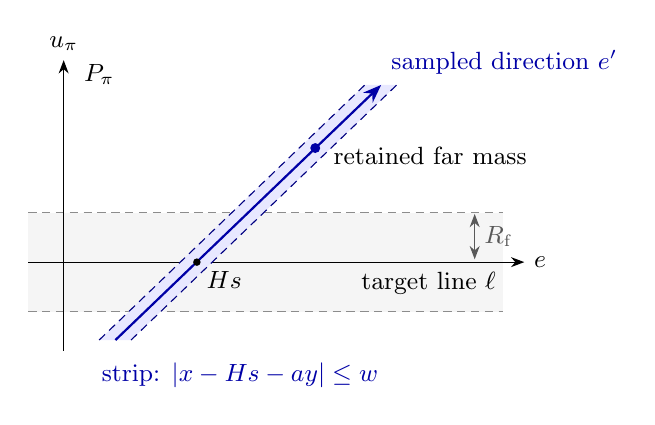
\begin{tikzpicture}[scale=0.9,>=Stealth,font=\small]
 \fill[black!4] (-0.5,-0.7) rectangle (6.2,0.7);
 \draw[densely dashed,black!45] (-0.5,0.7)--(6.2,0.7);
 \draw[densely dashed,black!45] (-0.5,-0.7)--(6.2,-0.7);
 \draw[->] (-0.5,0)--(6.5,0) node[right] {$e$};
 \draw[->] (0,-1.25)--(0,2.85) node[above] {$u_\pi$};
 \node[below] at (5.15,0) {target line $\ell$};
 \fill[blue!9] (0.5,-1.1)--(0.95,-1.1)--(4.7,2.5)--(4.25,2.5)--cycle;
 \draw[blue!65!black,thick,->] (0.73,-1.1)--(4.48,2.5)
       node[above right] {sampled direction $e'$};
 \draw[blue!50!black,densely dashed] (0.5,-1.1)--(4.25,2.5);
 \draw[blue!50!black,densely dashed] (0.95,-1.1)--(4.7,2.5);
 \fill (1.88,0) circle (1.5pt);
 \node[below right] at (1.88,0) {$Hs$};
 \fill[blue!65!black] (3.55,1.61) circle (2pt);
 \node[right] at (3.67,1.5) {retained far mass};
 \draw[<->,black!65] (5.8,0.04)--(5.8,0.68)
       node[midway,right] {$R_{\mathrm f}$};
 \node[anchor=west] at (0.15,2.65) {$P_\pi$};
 \node[anchor=west,blue!65!black] at (0.4,-1.6)
       {strip: $|x-Hs-ay|\leq w$};
\end{tikzpicture}
\caption{Geometry in the bin plane $P_\pi$ (schematic projection).
The shaded horizontal band is the near region removed in
\eqref{eq:geometry-near-mass}; the thin sloping strip contains the
sampled tube after enlargement. Since its direction is separated
from the target, only a controlled length lies in the near band.
The true plate also has thickness $w$ perpendicular to this picture.}
\label{fig:geometry-far}
\end{figure}

Because a sampled tube makes sine-angle at least $\delta$ with
$\ell$, the length of its width-$W$ portion within distance
$R_{\mathrm f}$ of $\ell$ is at most
$C\delta^{-1}(W+R_{\mathrm f})$. Covering it by radius-$O(W)$
balls gives the mass bound
\begin{equation}\label{eq:geometry-near-mass}
 C\delta^{-1}W(W+R_{\mathrm f})
 \leq C X^{c_0+2c_1}
       +CHX^{c_0+c_1-c_3}.
\end{equation}
Choose $c_3>A_{\mathrm r}+c_0+c_1$ by a large fixed margin, and
then require $H\gg X^{A_{\mathrm r}+c_0+2c_1}$. The bound in
\eqref{eq:geometry-near-mass} is less than half the lower bound in
\eqref{eq:geometry-local-richness}, uniformly for every sampled
tube. Integrating their retained richness against the sampling
law therefore gives
\begin{equation}\label{eq:geometry-strip-first-moment}
 \int_{Q_\pi^{\mathrm{far}}}F_\pi\,d\nu
 \geq cHX^{-A_{\mathrm r}}m_\pi.
\end{equation}
This step uses the richness of every neighboring tube against
$\nu$, including mass far from the point at which it was sampled.

Cauchy--Schwarz, \eqref{eq:geometry-strip-energy}, and
\eqref{eq:geometry-strip-first-moment} imply
\begin{equation}\label{eq:geometry-far-plate-mass}
 \nu(Q_\pi^{\mathrm{far}})
 \geq H^2X^{-K_0}m_\pi^{1-\gamma}
\end{equation}
for some $K_0\geq2A_{\mathrm r}+A_{\mathrm E}$, enlarged to absorb
fixed constants.

All planes $P_\pi$ pass through the same line $\ell$. At a point
$q$ at distance $\rho\geq R_{\mathrm f}$ from that line, the
condition $\dist(q,P_\pi)\leq w$ restricts $u_\pi$ to two azimuth
arcs of length $O(w/\rho)$. The two arcs account for opposite radial
directions. Since bins have size comparable to $H^{-1}$, their
overlap multiplicity is at most
\[
 C(1+Hw/R_{\mathrm f})\leq X^{A_{\mathrm O}},
 \qquad A_{\mathrm O}>c_2+c_3
\]
after a fixed enlargement. Take $H\gg X^{c_2+c_3}$ so that
$w\ll R_{\mathrm f}$. Summing
\eqref{eq:geometry-far-plate-mass}, using this overlap and
$\nu(\R^3)\lesssim H^2$, gives
\begin{equation}\label{eq:geometry-bin-concentration}
 \sum_\pi m_\pi^{1-\gamma}\leq X^{K_1}
\end{equation}
for a fixed $K_1>K_0+A_{\mathrm O}$. But
\[
 1=\sum_\pi m_\pi
 \leq (\max_\pi m_\pi)^\gamma
          \sum_\pi m_\pi^{1-\gamma}.
\]
Hence some bin has $m_\pi\geq X^{-K_1/\gamma}$. Its plane contains
the exact target line, and its width-$w$ plate has mass at least
\begin{equation}\label{eq:geometry-rich-plane}
 H^2X^{-K},\qquad
 K\geq K_0+(1-\gamma)K_1/\gamma.
\end{equation}
We have produced such a rich plane for every target tube.

\emph{5. Pack rich planes using both normal and offset separation.}
Return to a common origin at the center of the original domain.
Write each plane just obtained as
\[
 P_j=\{q:n_j\cdot q=b_j\},\qquad |n_j|=1,
\]
with $(n_j,b_j)$ identified with $(-n_j,-b_j)$. The width-$w$
plates, restricted to $\supp\nu$, all have mass at least
$\lambda H^2$, where $\lambda=X^{-K}$. Let
$C_{\mathrm t}$ be a fixed bound for $\nu(\R^3)/H^2$.

Choose an angular threshold $\vartheta=X^{c_4}/H$, with
$c_4>2c_2+2K$ by a sufficiently large fixed margin. If the
projective angle between two normals is at least $\vartheta$,
the intersection of their width-$w$ plates inside the domain is
contained in a box with dimensions
\[
 O(H)\ \times\ O(w)\ \times\
 O\bigl(w/|\sin\angle(n_i,n_j)|\bigr).
\]
Here projective angles lie in $[0,\pi/2]$, and $\vartheta\ll1$.
Unit-ball covering thus gives
\begin{equation}\label{eq:geometry-plate-intersection}
 \nu(Q_i\cap Q_j)
 \leq C H^2X^{2c_2-c_4}
 \leq \varepsilon H^2,
 \qquad \varepsilon\leq\lambda^2/(2C_{\mathrm t}).
\end{equation}
For a pair of normals at projective angle below $\vartheta$, align
their signs. Changing the normal then changes its defining linear
function by at most $C H\vartheta$ on the domain. Choose an offset
threshold
\begin{equation}\label{eq:geometry-offset-threshold}
 \Delta=X^{c_5}>2w+CH\vartheta,
 \qquad c_5>\max\{c_2,c_4\}
\end{equation}
with sufficiently large fixed margins. Such a close-normal pair
with $|b_i-b_j|\geq\Delta$ has disjoint plates on the domain.

Select a maximal sublist in which every pair is separated either
by projective normal angle at least $\vartheta$, or, after aligning
closer normals, by offset at least $\Delta$. Finiteness makes this
selection immediate. If the list has length $N$, set
$G=\sum_{j=1}^N\mathbf1_{Q_j}$. Its first and second moments obey
\[
 \int G\,d\nu\geq N\lambda H^2,
 \qquad
 \int G^2\,d\nu\leq C_{\mathrm t}NH^2+\varepsilon N^2H^2.
\]
Cauchy--Schwarz and the total mass bound give
\[
 N^2\lambda^2
 \leq C_{\mathrm t}^2N+C_{\mathrm t}\varepsilon N^2.
\]
By the choice in \eqref{eq:geometry-plate-intersection}, the last
term is absorbed, and
\begin{equation}\label{eq:geometry-plate-count}
 N\leq2C_{\mathrm t}^2\lambda^{-2}\leq X^{O(1)}.
\end{equation}

Maximality says that each original plane is close to a selected
one in both its projective normal and its aligned offset. On the
entire bounded range of relevant trajectory segments, this means
that its central line lies within
$\Delta+CH\vartheta=X^{O(1)}$ of the selected plane. Enlarge the
selected plates accordingly. If $n_0$ is the original normal of
the plane through the target line and $n$ is the aligned selected
normal, then
\[
 n_0\cdot(2\omega_T,1)=0,\qquad |n-n_0|\lesssim\vartheta.
\]
Bounded velocity now gives
$|n\cdot(2\omega_T,1)|\lesssim X^{c_4}/H$, proving
\eqref{eq:src11}. Offset control is essential for containment of
the segment; angular control supplies the asserted directional
bound.

\emph{Constant hierarchy.}
Here is one complete order of choices. First fix the data in the
proposition and $M=100$. Choose $c_0,c_1$ so that
\[
 c_0\eta>A_{\mathrm a},\qquad
 (M-1)c_1>A_{\mathrm r},
\]
with fixed margins that give the two required half-mass losses.
Next choose $c_2>c_0+c_1$, followed by
\[
 A_{\mathrm F}>A_{\mathrm r}+2c_1+A_{\mathrm a},\qquad
 A_{\mathrm I}>3c_2+c_0,\qquad
 A_{\mathrm E}>A_{\mathrm I}+A_{\mathrm F}/(1+\eta),
\]
with sufficient fixed margins for
\eqref{eq:geometry-joint-frostman}--\eqref{eq:geometry-strip-energy}.
Choose
\[
 c_3>\max\{c_2,A_{\mathrm r}+c_0+c_1\},
\]
and then choose $A_{\mathrm O},K_0,K_1,K$ as in
\eqref{eq:geometry-far-plate-mass}--\eqref{eq:geometry-rich-plane}.
Choose $c_4>2c_2+2K$ to ensure
\eqref{eq:geometry-plate-intersection}, and then
$c_5>\max\{c_2,c_4\}$ to ensure
\eqref{eq:geometry-offset-threshold}. Choose $C'$ larger than
$c_5,c_4,2K$, with a fixed margin absorbing the final widths,
counts, and direction constants. Finally take
\[
 A_*>\max\{A_{\mathrm r}+c_0+2c_1,\ c_2+c_3,\ c_0,\ c_4,\ C'\},
\]
and $C_*$ sufficiently large. Every strict inequality here includes
an additional fixed margin if necessary for the fixed constants.
All choices precede $X,H$; in particular no exponent depends on
the number of tubes or on an azimuth-bin mass.
\end{proof}

\section{The dyadic distribution estimate}\label{sec:dyadic}

The sparse estimate supplies a gain when every packet meets little measure.
For a general array, we first remove sparse packets and narrow angular
contributions.  The remaining packets lie in a controlled collection of
plates.  The main analytic step then replaces all intermediate packet scales
by a single family at a shorter scale, to which the bilinear frame estimate
applies.

\begin{theorem}[Dyadic distribution bound]\label{thm:distribution}
There are fixed $p>2$ and $\sigma>0$ with the following property.
Let $U$ be a finite sum of the atoms in \eqref{eq:src5}, of packet size
$L\geq1$, with $\sum_\alpha|c_\alpha|^2\leq1$.  Suppose that $\mu$ is
supported in a spatial box of side $O(L^2)$ and in $|t|\leq L^2$, that
$\mu(B_r)\leq mr^2$ for every ball of radius $r\geq1$, and that
\eqref{eq:src6} holds for every label, with $1\leq D\leq L$.
Then, for every $g>0$,
\begin{equation}\label{eq:src12}
 \mu(A)\leq C mL^4D^{-\sigma}g^{-p},
 \qquad A=\{z:|U(z)|\geq\lambda\},\qquad
 \lambda=gL^{-4/3}.
\end{equation}
The constant is uniform in $L,D,g,m$ and the size of the array.  It may
depend on the fixed packet class, including sufficiently many finite
profile derivative bounds.  For an arbitrary coefficient array, the right
side is multiplied by $\|c\|_{\ell^2}^p$.
\end{theorem}

We fix the packet class throughout the proof.  In particular, its frequency
square, phase-space counting constant, profile support, and required
derivative bounds are fixed.  Recursive cap scalings will be performed in
the original, unrotated coordinates, using squares and retaining only the
specified subarray.  This preserves the class, including its derivative
bounds.  Rotations used later are only in nonrecursive estimates.  The
regularity order can be chosen after all small exponents: the saving $c_s$
in Proposition~\ref{prop:sparse}, the geometric powers in
Proposition~\ref{prop:rich}, and the separation power in
Theorem~\ref{thm:frame} do not increase when additional profile regularity
is required.

\subsection{Parameters and recursive estimates}

Write $c_s$ for the saving in \eqref{eq:src7}, and $p_0>2$ for the exponent
in \eqref{eq:src9} and \eqref{eq:src10}. Choose
$2<p_{\max}<\min(p_0,3)$ and then $\eta>0$ so small that
\begin{equation}\label{eq:dyadic-gamma}
 \gamma_0=1-p_{\max}/3-p_{\max}\eta>0.
\end{equation}
We introduce the parameters used in the construction and work conditionally
on the inequalities below. Their compatible order of choice will be checked
after the estimates, when the losses determining them have been identified.
For fixed constants $B,C_a$ and a small exponent $u>0$, set
\begin{equation}\label{eq:dyadic-parameters}
 X=BD,\qquad D_*=BD^2,\qquad \delta_0\asymp X^{-u},
 \qquad a\asymp X^{C_a},\qquad h=L/a.
\end{equation}
Round $\delta_0$ and $h$ to convenient dyadic scales, changing only fixed
constants. The parameter $D_*$ will be used in the sparse-packet deletion;
$\delta_0$ is the upper scale for cap recursion. The shorter packet scale
$h$ will be used after the geometric reduction.

We split the proof at $D=L^\kappa$, with $\kappa>0$ sufficiently small.
In the range $D<L^\kappa$, we require $h$ to dominate the fixed powers
of $X$ occurring below, after enlarging a fixed base scale $L_0$. We also require
$2<p\leq p_{\max}$ and $0<\sigma\leq1$ with
\begin{equation}\label{eq:dyadic-exponent-conditions}
 \sigma+\frac{4(p-2)}{3\kappa}<c_s,\qquad
 C_fu+C_g(p-2)+\sigma<c_s,\qquad
 \sigma<u\gamma_0.
\end{equation}
Here $C_g$ is the fixed exponent separating the large levels
$g\geq X^{C_g}$ from the remaining levels, and $C_f$ is a fixed loss exponent, independent of $u$. The frame
application below will determine a sufficient value of $C_f$ for
\eqref{eq:dyadic-final-energy}. All three
inequalities have strict margins. We take $B$ sufficiently large for the
recursive terms to contract, and choose the overall induction constant
only after the nonrecursive estimates have been obtained.

Two elementary estimates start the induction.  At a point, compact support
allows only $O(L^2)$ labels, each atom is $O(L^{-1})$, and hence
\begin{equation}\label{eq:dyadic-sup}
 \|U\|_\infty\lesssim\|c\|_{\ell^2}.
\end{equation}
Also $\mu(\supp\mu)\lesssim mL^4$.  Thus all bounded scales are covered
by a constant depending on $L_0$.  When $D\geq L^\kappa$, unit-cube mass
is $O(m)$, so Proposition~\ref{prop:sparse} gives
\[
 \int|U|^2\,d\mu
 \leq C m^{1/3}\sum_q\mu(q)^{2/3}\sup_q|U|^2
 \lesssim_\kappa mL^{4/3}D^{-c_s}.
\]
Chebyshev therefore gives $CmL^4D^{-c_s}g^{-2}$.  A nonempty level set
has $g\lesssim L^{4/3}$ by \eqref{eq:dyadic-sup}; the first inequality
in \eqref{eq:dyadic-exponent-conditions} implies
$D^\sigma g^{p-2}\lesssim D^{c_s}$.  This proves
\eqref{eq:src12} in the sparse range independently of induction.

For $D<L^\kappa$, use outer induction on dyadic ranges of $L$ and inner
induction on the number of iterations of $d\mapsto Bd^2$ needed to reach
$L^\kappa$.  Thus the result is available at a fixed smaller packet
scale, and at the present scale with parameter $D_*$.  For sufficiently
large $L$ in this range, $D_*\leq L$; it suffices to have
$BL^{2\kappa}\leq L$.  Denote the inductive constant by $C_{\rm ind}$.
We will bound recursive contributions by a fixed fraction of
$C_{\rm ind}mL^4D^{-\sigma}g^{-p}$ and all other contributions by a
constant independent of $C_{\rm ind}$.

\begin{lemma}[Cap gain]\label{lem:dyadic-cap-gain}
For any subarray in a frequency square of side comparable to $r$, where
$L^{-1}\lesssim r\leq\delta_0$, outer induction gives
\begin{equation}\label{eq:dyadic-cap-gain}
 \mu\{|U_{\mathcal C}|\geq r^\eta\lambda\}
 \leq C_{\rm cap}C_{\rm ind}mL^4g^{-p}
 r^{1-p/3-p\eta}
 \Big(\sum_{\alpha\in\mathcal C}|c_\alpha|^2\Big)^{p/2}.
\end{equation}
The estimate holds for any submeasure of $\mu$, with the same upper ball
parameter.  At the smallest scales choose comparable squares so that
the child packet size is at least $1$.
\end{lemma}
\begin{proof}
For a square centered at $v$, use
$(x',t')=(r(x-2vt),r^2t)$, up to fixed normalization conventions.  The
child packet size is $L'=rL$, the field factor is $r$, and the pushed
measure has ball parameter $m'\leq Cm r^{-3}$.  The new threshold
parameter is comparable to $g r^{1/3+\eta}$, since
\[
 r^{-1}r^\eta gL^{-4/3}
   =g r^{1/3+\eta}(rL)^{-4/3}.
\]
After a fixed inflation of $m'$, covering tubes and their transverse
annuli supplies \eqref{eq:src6} with $D=1$; equivalently
$m'(L')^3\asymp mL^3$.  The time interval is still
$|t'|\leq(L')^2$.  Partition the transformed spatial range into boxes
of side comparable to $(L')^2$.  A compact child packet meets only
boundedly many such boxes during this time interval.  If their relevant
coefficient energies are $e_j$, then
$\sum_j e_j\lesssim\sum_{\mathcal C}|c_\alpha|^2$ and
$\sum_j e_j^{p/2}\leq(\sum_j e_j)^{p/2}$.  Consequently outer induction
costs no number of boxes.  Its dimensional factor is
\[
 (mr^{-3})(rL)^4(g r^{1/3+\eta})^{-p}
  =mL^4g^{-p}r^{1-p/3-p\eta},
\]
as asserted.  These parabolic transformations translate the pairs
$(b_\alpha/L,L\omega_\alpha)$ and leave the normalized profiles
unchanged.  Enclosing a specified cap in a comparable square does not
add any other labels.
\end{proof}

We need the same estimates when the output point determines a prefix of
the array.  The next elementary device avoids a loss depending on the
number of labels. It adapts the dyadic input-energy decomposition of
Christ and Kiselev \cite[Theorem~1.1 and its proof in Section~2]{CK01}
to the weak-type block estimates on restricted submeasures used here.
We give the proof for these hypotheses, rather than applying their
maximal theorem as a black box.

\begin{lemma}[Energy truncation]\label{lem:dyadic-prefix}
Let a finite coefficient array be ordered, with total energy $E$, and let
each output point select a prefix ending between whole coefficients.
Suppose the distribution estimate for every block, on the submeasure
where that block is selected, has right side
$K t^{-p}\|c_{\rm block}\|_{\ell^2}^p$, where $p>2$.
The field formed from the selected prefix then satisfies the same
estimate with right side $C_p Kt^{-p}E^{p/2}$.
\end{lemma}
\begin{proof}
Zero coefficients may be omitted, and $E=0$ is trivial.  Place successive
intervals of lengths $|c_\alpha|^2/E$ in $[0,1]$.  For a dyadic interval
$I\subset[0,1]$, apportion $c_\alpha$ by the fraction of its interval
lying in $I$.  If that fraction is $f_{\alpha,I}$, its apportioned
energy obeys
\[
 \sum_\alpha |f_{\alpha,I}c_\alpha|^2
 \leq\sum_\alpha f_{\alpha,I}|c_\alpha|^2=E|I|.
\]
These apportioned blocks satisfy the assumed distribution estimate, up
to a constant depending on $p$. Each is either a single apportioned
coefficient or the sum of a whole interior block and at most two
fractional endpoint coefficients. Homogeneity gives the estimate for
the fractional singletons. Split the threshold equally among these at
most three pieces and use
$\sum_i\|c_i\|_2^p\leq(\sum_i\|c_i\|_2^2)^{p/2}$;
the pieces have disjoint coefficient supports. The resulting bound uses
exactly the apportioned energy above.

Every prefix interval $[0,s)$ is a disjoint union of at most one dyadic
interval at each depth $k\geq0$.  Every coefficient contributing to a
used interval belongs to the prefix, because $s$ is between whole
coefficient intervals.  The sum of these block fields equals the prefix
field, also when the binary expansion is infinite; the original array
is finite and the coefficient fractions sum exactly.

Choose $0<\epsilon<(p/2-1)/p$ and positive thresholds
$t_k=c_\epsilon t2^{-\epsilon k}$ with $\sum_k t_k=t$.
If a prefix field exceeds $t$, some used block exceeds $t_k$.
There are at most $2^k$ blocks at depth $k$, each with energy at most
$E2^{-k}$.  Restricting the measure separately to points using a block,
and summing the distribution bounds, gives
\[
 3^pKt^{-p}E^{p/2}c_\epsilon^{-p}
 \sum_{k\geq0}2^{k(1-p/2+p\epsilon)}
 \leq C_pKt^{-p}E^{p/2}.
\]
This argument also applies inside each fixed frequency cap, with its
own total energy $E$.
\end{proof}

\subsection{Peeling to a common rich measure}

Starting with $A$, repeatedly perform the following two deletions.
First remove all labels whose smoothed mass against the measure on the
current set is less than $mL^3/D_*$.  Next remove every point at which
the remaining physically neighboring labels do not support a probability
law with direction-ball bounds
\begin{equation}\label{eq:dyadic-angular-law}
 \mathbb P\{\omega\in B_r(v)\}
 \leq C_{\rm ang}\delta_0^{-\eta}r^\eta,
 \qquad L^{-1}\leq r\lesssim1.
\end{equation}
Here a physical neighbor means that the point is within a fixed multiple
of $L$ of the packet trajectory; the multiple contains the compact
profile support.  Directions and frequency centers are interchangeable
up to fixed constants on the bounded frequency square.

The angular test can use a finite dyadic label tree, ending at scale
comparable to $L^{-1}$, so it depends measurably on one of finitely many
incidence patterns.  If a round deletes points but no subsequent label,
the angular test is unchanged and no further point can be deleted.
Since there are finitely many labels, the process terminates.  Write
$A_\infty$ for its stabilized set and $\mathcal R$ for its surviving
labels.  At termination all labels in $\mathcal R$ satisfy
\begin{equation}\label{eq:dyadic-rich-common}
 \int_{A_\infty}
 (1+|x-b_\alpha-2\omega_\alpha t|/L)^{-M}\,d\mu
 \geq mL^3/D_*;
\end{equation}
every point of this same set satisfies \eqref{eq:dyadic-angular-law}
using physically neighboring labels in $\mathcal R$.

To estimate what was deleted, order removed labels by their removal
round, breaking ties arbitrarily.  Each original point selects the
prefix removed before it exits, including all labels removed in its exit
round; a point of $A_\infty$ selects all removed labels.  Let $P(z)$ be
this prefix field.  For any binary block in
Lemma~\ref{lem:dyadic-prefix}, restrict the measure to points whose
prefix uses the block.  Such points were still present when each
contributing label was removed.  By monotonicity of the smoothed
integral, every label in that block satisfies \eqref{eq:src6} with
$D_*$.  Inner induction and Lemma~\ref{lem:dyadic-prefix} therefore
give, for any fixed small $c>0$,
\begin{equation}\label{eq:dyadic-prefix-exception}
 \mu\{|P|\geq c\lambda\}
 \leq C_p C_{\rm ind}mL^4D_*^{-\sigma}g^{-p}.
\end{equation}
This restriction of measure is essential: a removed label need not be
sparse on all of the original set.

For both the original field and this prefix field, also remove the
exceptional sets where a dyadic cap contribution at any scale
$L^{-1}\lesssim r\leq\delta_0$ exceeds $r^\eta\lambda$.
Lemma~\ref{lem:dyadic-cap-gain} and, for prefixes,
Lemma~\ref{lem:dyadic-prefix}, imply a total cost
\begin{equation}\label{eq:dyadic-cap-exceptions}
 C' C_{\rm ind}mL^4g^{-p}\delta_0^{\gamma_0}.
\end{equation}
Indeed cap energies at each scale partition the original energy, so
their $p/2$ powers sum to at most $1$, and
$1-p/3-p\eta\geq\gamma_0$ makes the dyadic scale sum geometric.

\begin{lemma}[The angular test cannot fail elsewhere]
\label{lem:dyadic-flow}
Outside the exceptions in \eqref{eq:dyadic-prefix-exception} and
\eqref{eq:dyadic-cap-exceptions}, an original point cannot exit in an
angular deletion.  On a surviving such point,
$|U_{\mathcal R}|\geq c\lambda$ for an absolute $c>0$.
\end{lemma}
\begin{proof}
At a proposed exit, subtract the selected prefix from $U$.  The
remaining field has modulus at least a fixed fraction of $\lambda$,
and every fine cap sum has modulus at most $2r^\eta\lambda$.
Only physically neighboring remaining labels can contribute at the
point.

Mark the terminal cells of the finite direction tree that contain such
a neighboring label.  Give unmarked terminal cells capacity zero,
fine cells of side $r\leq\delta_0$ capacity $r^\eta$, and coarser cells
capacity $1$.  A cut covering the marked leaves either contains a
coarse cell, and hence has capacity at least $1$, or consists of fine
cells.  In the latter case its cell fields sum to the remaining field,
so the triangle inequality gives total capacity at least an absolute
positive constant.  Nonneighboring labels in these cells contribute
zero at the point.

For completeness, the maximal mass that can pass through a node is
the minimum of its capacity and the sum of the maximal masses of its
children.  Induction up the finite tree shows that this is the minimum
cut capacity.  Thus a mass bounded below can be sent from the root to
marked leaves.  Choose a neighboring label in each such leaf and
normalize the resulting flow to a probability.  A fine cell of side $r$
then has probability $O(r^\eta)$.  A ball of radius $r\geq L^{-1}$ is
covered by boundedly many cells of comparable size.  At coarser scales
$r\geq\delta_0$, the desired bound follows from
$\delta_0^{-\eta}r^\eta\geq1$.  Taking $C_{\rm ang}$ large enough
gives \eqref{eq:dyadic-angular-law}, a contradiction to the exit test.
The assertion about the final field follows by subtracting its prefix.
\end{proof}

Relative to the target with constant $C_{\rm ind}$, the recursive costs
so far are bounded by fixed multiples of
\begin{equation}\label{eq:dyadic-contraction}
 (D_*/D)^{-\sigma}=X^{-\sigma},\qquad
 D^\sigma\delta_0^{\gamma_0}
 \lesssim D^\sigma X^{-u\gamma_0}.
\end{equation}
The later single-cap exceptions have the second form as well.  The last
inequality in \eqref{eq:dyadic-exponent-conditions} and a sufficiently
large $B$ make the sum of all these costs less than, say, half the
target.  Their constants include the fixed prefix constant $C_p$, but
do not include any of the final nonrecursive constants.

We apply geometry to $\mu|_{A_\infty}$ itself, before subtracting any of
the proof-only exceptional sets.  Equations
\eqref{eq:dyadic-angular-law} and \eqref{eq:dyadic-rich-common}
therefore hold for the same measure.  Subsequent upper bounds may use
the original $\mu$: its ball and sparsity upper bounds still hold for
every surviving label.

\subsection{Plates and coarse frequency intervals}

Divide physical coordinates by $L$, and divide $\mu|_{A_\infty}$ by
$mL^2$.  In the notation of Proposition~\ref{prop:rich}, $H=L$,
the richness is at least $L/D_*\geq L/X^2$, and the angular constant
in \eqref{eq:dyadic-angular-law} is at most a fixed power of $X$.
The required comparisons $X^C\ll H$ hold by the choice of $\kappa$.
Proposition~\ref{prop:rich} assigns every surviving tube to one of at
most $X^{C_1}$ plates of width $X^{C_1}$ in these coordinates, with
\[
 |n\cdot(2\omega,1)|\leq X^{C_1}/L.
\]
Enlarge the plates by a fixed polynomial factor to contain the physical
packet supports in the domain.  All assignments are disjoint at the
level of coefficient labels.

The spatial component $n_x$ of such a unit normal is bounded below.
Indeed $|\omega|\leq C$, so if $|n_x|$ were sufficiently small, then
$|n_t+2n_x\cdot\omega|$ would be bounded below by an absolute constant,
contrary to the displayed estimate for large $L$.  Thus the assigned
frequencies lie in a strip of width $X^{O(1)}/L$, which can be partitioned
into polynomially many strips of width $O(L^{-1})$.  If the total number
of resulting arrays is $N\leq X^{C_2}$, the triangle inequality and
Proposition~\ref{prop:strip} give
\begin{equation}\label{eq:dyadic-large-level}
 \mu\{|U_{\mathcal R}|\geq c\lambda\}
 \lesssim mL^4N^{p_0}g^{-p_0}
       \sum_{j=1}^N\|c_j\|_{\ell^2}^{p_0}
 \leq X^{C_3}mL^4g^{-p_0}.
\end{equation}
Choosing $C_g(p_0-p_{\max})>C_3+1$ makes this at most a fixed multiple
of the target whenever $g\geq X^{C_g}$.  For $g<D^{-1}$, total mass
suffices, since $D^{-\sigma}g^{-p}\geq D^{p-\sigma}\geq1$ after
decreasing $\sigma$ if necessary.  We henceforth work in
\begin{equation}\label{eq:dyadic-middle-levels}
 D^{-1}\leq g\leq X^{C_g}.
\end{equation}

Discard intersections of enlarged plates whose projective normal
directions differ by at least a constant multiple of $a/L$.  For two
plates of normalized width $w\leq X^{C_4}$ and normal separation
$\beta$, their intersection is in a box of length $O(L)$ and transverse
sides $O(w)$ and $O(w/\beta)$.  Its normalized mass is at most
$X^{O(1)}L/\beta$ by unit-ball covering.  Summing over the polynomial
plate list, the discarded mass in the original coordinates is at most
\begin{equation}\label{eq:dyadic-plate-discard}
 mL^4X^{C_5}/a.
\end{equation}
Choose $C_a>C_5+1+C_gp_{\max}$, with room for fixed constants.  Then
\eqref{eq:dyadic-plate-discard} is bounded by the target throughout
\eqref{eq:dyadic-middle-levels}.

Partition projective normal directions into cells of diameter comparable
to $a/L$, with bounded overlap on balls of that radius.  At a retained
point all active plate normals have pairwise distance $O(a/L)$.
Consequently only boundedly many normal cells contribute, and at least
one cluster field has modulus at least $c\lambda$.  Relative to a
representative normal in each nonempty cell, its label frequencies lie
in a strip of width $O(a/L)=O(h^{-1})$.  The representative still has
spatial component bounded below, and this follows by perturbing the
previous direction inequality by $O(a/L)$.  The clusters partition the
surviving coefficient energy.

For each cluster separately rotate the spatial coordinates and remove
its central normal frequency by a bounded shear and modulation.
Write the resulting coordinates as $(x,y,t)$, with $x$ tangential and
$y$ normal.  Partition tangential label frequencies into coarse
intervals $\tau$ of length comparable to $\delta_0$, then into fine
intervals $\theta$ of length comparable to $h^{-1}$, using nested grids
and consistent endpoint assignments.  Each coarse array fits in a
comparable two-dimensional cap, because $h^{-1}\ll\delta_0$.
In applying Lemma~\ref{lem:dyadic-cap-gain}, enclose that array in an
unrotated square in the original coordinates, keeping only its labels.
At each scale bounded overlap of the enclosing squares, together with
the partitioned coefficient energy across clusters, gives a total
exceptional cost
\[
 C''C_{\rm ind}mL^4g^{-p}\delta_0^{\gamma_0}
\]
for the sets on which a coarse cluster field exceeds
$\delta_0^\eta\lambda$.  This is the further recursive cost already
allowed in \eqref{eq:dyadic-contraction}.

At any remaining point where a cluster is high, at least
$c\delta_0^{-\eta}$ distinct coarse intervals satisfy
\begin{equation}\label{eq:dyadic-significant-intervals}
 |U_\tau|\geq c'\delta_0\lambda.
\end{equation}
To see this, there are $O(\delta_0^{-1})$ coarse intervals, so the sum
of those below the displayed small threshold has modulus less than
half the cluster threshold if $c'$ is sufficiently small.  Each of the
others has modulus at most $\delta_0^\eta\lambda$, forcing the stated
number.  Full partition intervals are used throughout; the complement
estimate never discards only part of an interval field.

\subsection{Flattening all intermediate scales}

The cluster frequencies now lie in a strip of width $O(h^{-1})$, whereas
Proposition~\ref{prop:strip} at packet size $L$ requires width $O(L^{-1})$.
Splitting into thinner strips produced the large-level estimate, but paid
a fixed power of $X$. To handle the remaining levels, we instead make one
smooth packet out of each entire fine frequency array on each short
physical cell. We will apply Theorem~\ref{thm:frame} directly to these
packets and sum their energies. The construction uses only the general
compact profiles in \eqref{eq:src5}; no equation or exact Fourier
support is imposed on those profiles.

For a fine interval $\theta$ centered at $v_\theta$, put
\begin{equation}\label{eq:dyadic-child-coordinates}
 z'_\theta=F_\theta(x,y,t)
   =\big((x-2v_\theta t)/h,\ y/h,\ t/h^2\big).
\end{equation}
The central normal frequency has already been removed.  The array is
contained in a cap of size $O(h^{-1})$ and therefore has the form
\begin{equation}\label{eq:dyadic-child-field}
 U_\theta(x,y,t)
 =h^{-1}e^{i(xv_\theta-tv_\theta^2)}U'_\theta(z'_\theta),
\end{equation}
up to a common harmless modulation.  Here $U'_\theta$ is an array of
packet size $a=L/h$, with bounded frequencies and the original
coefficient norm.

Choose a fixed smooth partition of unity $\{\psi_T\}$ on the unit
lattice in $\R^3$, with bounded overlap and fixed enlarged supports.
Take a finite derivative order $N$ exceeding all later Sobolev and frame
requirements, and let
\[
 s_{\theta,T}
   =h^{-1}\max_{|\beta|\leq N}
       \sup_{z'\in T^*}|\partial^\beta U'_\theta(z')|,
\]
where $T^*$ is a fixed sufficiently large enlargement of $T$.  Enlarging
the fixed constant in this definition would give the same estimates.
Fix also a large polynomial decay power $P$, larger than $M+3$ and all
tail moments that will occur, and define
\begin{equation}\label{eq:dyadic-density}
 d_\theta(T)=\frac{1}{mh^3}
   \int(1+\dist(F_\theta(z),T))^{-P}\,d\mu(z).
\end{equation}
We abbreviate this to $d(T)$ when the cluster and $\theta$ are specified.
All coordinate changes push forward the measure without changing its
mass.  Their ball constants are uniformly bounded after the displayed
factor $h^3$.  In particular $d(T)\lesssim1$ by annular covering.

Only cells whose partition supports meet the testing domain need be
retained.  The associated summand
\begin{equation}\label{eq:dyadic-composite-packet}
 e^{i(xv_\theta-tv_\theta^2)}
 h^{-1}\psi_T(z'_\theta)U'_\theta(z'_\theta)
\end{equation}
is a single composite packet: it has tangential width $O(h)$, time
length $O(h^2)$, localized dependence on $y/h$, and all required
normalized derivatives bounded by $Cs_{\theta,T}$.

There are two energy bounds to retain. On a time interval of length $h^2$,
spatial almost orthogonality controls the total squared amplitudes of the
composite packets. Over the full time range, the sparse estimate controls
the same amplitudes weighted by $d(T)^{2/3}$. The first bound will supply
the large threshold-to-envelope ratios required by the frame theorem;
the second will retain the factor $D^{-c_s}$ when the frame estimates are
summed.

\begin{lemma}[Flattened energy estimates]\label{lem:dyadic-flattening}
For a time interval $J$ of length $h^2$, let $\mathcal T(J)$ denote the
boundedly many native time-cell layers that can contribute on $J$.
Summing over the disjoint fine arrays, and also over clusters when
needed, one has
\begin{equation}\label{eq:src13}
 \begin{aligned}
 \sum_{\theta,\,T\in\mathcal T(J)}s_{\theta,T}^2
     &\lesssim h^{-2},\\
 \sum_{\theta,T}d(T)^{2/3}s_{\theta,T}^2
     &\lesssim_B h^{-2}a^{4/3}D^{-c_s}.
 \end{aligned}
\end{equation}
The right sides are multiplied by the total original coefficient
energy if it is not normalized to be at most $1$.
\end{lemma}
\begin{proof}
We first justify spatial almost orthogonality for arbitrary smooth
packet profiles.  At native time $t'=O(a^2)$, a child atom and all its
fixed derivatives have spatial support within $O(a)$ of its transported
intercept $b'_\alpha+2\omega'_\alpha t'$.  Spatial integration by
parts in the difference of the carrier frequencies gives Gram entries
bounded by
\begin{equation}\label{eq:dyadic-gram}
 C_N(1+a|\omega'_\alpha-\omega'_\beta|)^{-N},
\end{equation}
and the entries vanish unless the transported intercepts differ by
$O(a)$.  The joint centers
\[
 (b'_\alpha/a,a\omega'_\alpha)
 \longmapsto
 \big(b'_\alpha/a+2(t'/a^2)a\omega'_\alpha,
      a\omega'_\alpha\big)
\]
undergo a uniformly bounded shear.  Thus their phase-space counts remain
bounded.  Summing \eqref{eq:dyadic-gram} over these centers gives
uniformly summable Gram rows when $N$ is sufficiently large.  It follows
that, for every required derivative,
\[
 \|\partial^\beta U'_\theta(\cdot,t')\|_{L^2(\R^2)}^2
 \lesssim \sum_{\alpha\in\theta}|c_\alpha|^2.
\]
Time derivatives are included: bounded child frequencies and factors
$a^{-1}$ or $a^{-2}$ from differentiating profiles preserve the same
packet bounds.  Unit-cell Sobolev estimates, bounded overlap of the
enlarged cells, and integration over the $O(1)$ native time layers in
$J$ now give the first assertion of \eqref{eq:src13}.  Summing the
coefficient energies across fine arrays and clusters costs at most $1$.

For the second assertion, let $\mu_\theta=F_{\theta\#}\mu$ in the
coordinates of the relevant cluster.  Covering the inverse image of a
ball shows that its ball parameter is at most $Cmh^3$ for radii at
least $1$.  For every child label, the transverse ratio in
\eqref{eq:src6} is unchanged by \eqref{eq:dyadic-child-coordinates},
and
\begin{equation}\label{eq:dyadic-child-moment}
 (mh^3)a^3/D=mL^3/D.
\end{equation}
Thus $\mu_\theta$ satisfies the same sparsity condition with $D$ after
a fixed inflation of its ball parameter.

Convolve $\mu_\theta$ with $K_P(z')=(1+|z'|)^{-P}$ and restrict the
resulting measure to $|t'|\leq C'a^2$, with a fixed enlargement sufficient
for the cells and derivatives in use.  Call the resulting measure
$\widetilde\mu_\theta$.  Its ball parameter remains $Cmh^3$.  Its
smoothed tube moments are still bounded as in
\eqref{eq:dyadic-child-moment}: translating a child tube kernel by $w$
changes it by at most a factor $C(1+|w|)^M$, and
\[
 \int_{\R^3}(1+|w|)^{M-P}\,dw<\infty.
\]
Every relevant unit cell $q$ in a fixed enlargement of $T$ has
\begin{equation}\label{eq:dyadic-convolved-cell}
 \widetilde\mu_\theta(q)\gtrsim mh^3d(T),
\end{equation}
after using the time enlargement; this follows by comparing the kernel
at all points of $q$ with its distance to $T$.

Apply Proposition~\ref{prop:sparse}, including its derivative version,
at packet size $a$ to $U'_\theta$ and
$\widetilde\mu_\theta$.  Unit cells in $T^*$, of which there are
boundedly many, control the suprema defining $s_{\theta,T}$.
Using \eqref{eq:dyadic-convolved-cell} and dividing out
$(mh^3)^{2/3}$ yields
\[
 \sum_T d(T)^{2/3}s_{\theta,T}^2
 \lesssim h^{-2}a^{4/3}D^{-c_s}
       \sum_{\alpha\in\theta}|c_\alpha|^2.
\]
The transformed spatial domain may exceed size $a^2$.  To use the local
form of the sparse estimate, divide it into boxes of side comparable to
$a^2$ and retain only intersecting compact child packets.  Each such
packet meets boundedly many boxes on $|t'|\leq C'a^2$; summing the
squared estimates therefore uses only bounded total coefficient energy.

This application requires a fixed positive-power lower bound on $D$ in
terms of $a$.  By $a\asymp(BD)^{C_a}$ and $a\geq D$, we have
$a^{1/(2C_a+2)}\leq D\leq a$ once $D$ exceeds a constant depending on
$B$.  Use this fixed exponent in Proposition~\ref{prop:sparse}.
For the remaining bounded values of $D$, also $a$ is bounded in terms
of $B$.  The first assertion summed over $O(a^2)$ time layers, and
$d(T)\lesssim1$, gives the second assertion with a different allowed
constant.  Finally sum over the partitioned coefficient arrays.
\end{proof}

We sort the cells into dyadic density bands
$d(T)\asymp d_\ell$, where $d_\ell=d_{\max}2^{-\ell}$,
$\ell\geq0$, and $d_{\max}$ is a fixed upper bound.  Shifting this
index by a fixed amount has no effect.  Only $O(\log h)$ bands need
occur.  Indeed if the total measure of the domain is already less than
$mL^4D^{-\sigma}g^{-p}$ there is nothing to prove.  Otherwise, for a
relevant cell the transformed domain diameter is $O(L^2/h)$, and the
strictly positive weight in \eqref{eq:dyadic-density} gives
\begin{equation}\label{eq:dyadic-density-lower}
 d(T)\gtrsim (mh^3)^{-1}\mu(\text{domain})
                   (1+CL^2/h)^{-P}
 \gtrsim a^{4-2P}h^{1-P}D^{-\sigma}g^{-p}.
\end{equation}
Here $L=ah$, and fixed powers of $a,D,g$ are bounded by fixed powers of
$X$, which in turn are bounded by fixed powers of $h$.  Thus
$d(T)\geq c_B h^{-C}$ with a fixed $C$.  This band count will only be
used with a power gain in $h$; it will not remain in the final bound.

\subsection{Two bands and the bilinear frame estimate}

For every coarse interval satisfying
\eqref{eq:dyadic-significant-intervals}, summably split its threshold
over the density bands.  At least one band field then has modulus at
least
\begin{equation}\label{eq:dyadic-band-level}
 A_\ell=c\delta_0(1+\ell)^{-2}\lambda.
\end{equation}
The constant $c>0$ is fixed sufficiently small that the sum of these
thresholds is less than the significant-interval threshold.  Choose one
such band for each significant interval. Fix a sufficiently large exponent
$C_d$, to be chosen in the tiny-band estimate below. If one selected band has
$d<X^{-C_d}$, pair its interval with a separated significant interval.
Otherwise there are only $O(C_d\log X)$ selected bands.  By increasing
$B$, the number $c\delta_0^{-\eta}$ in
\eqref{eq:dyadic-significant-intervals} exceeds a sufficiently large
multiple of this band count.  Pigeonholing gives two separated coarse
intervals with the same band.  Here ``separated'' means distance at least
a fixed multiple of $\delta_0$; excluding a bounded number of neighboring
intervals suffices.  The list of significant intervals is also large
enough to supply the partner in the tiny-band case.

Partition time into intervals $J$ of length $h^2$.  For each cluster,
$J$, separated pair $(\tau_1,\tau_2)$, and selected bands
$(\ell_1,\ell_2)$, form the measurable subset where both band fields
exceed the corresponding levels in \eqref{eq:dyadic-band-level}.
Restrict to the high points under consideration if desired.  Denote its
mass by $M_0$, and put
\begin{equation}\label{eq:dyadic-class-energy}
 E_i=\sum_{\substack{\theta\subset\tau_i,\ T\in\mathcal T(J)\\
                         d(T)\asymp d_i}}
                 s_{\theta,T}^2,
 \qquad d_i=d_{\ell_i},\qquad i=1,2.
\end{equation}
The witness subsets need not be disjoint; we use an upper bound on their
sum of masses.  There are at most $X^{C_6}(\log h)^2$ relevant tuples:
the cluster list and interval pairs have polynomial size in $X$, and
the time partition contributes $O(a^2)$ intervals.

Tuples with
\begin{equation}\label{eq:dyadic-small-mass}
 M_0\leq mh^{4-1/12}
\end{equation}
have total mass at most
$X^{C_6}(\log h)^2mh^{4-1/12}$.  Relative to the target this is at most
\[
 C X^{C_6+\sigma+C_gp_{\max}}
          a^{-4}h^{-1/12}(\log h)^2,
\]
which is bounded, and can be made small at large scales, by the choice
of $\kappa$.  This discard counts tuples before normal spatial slabs
are introduced, so it incurs no number of slabs.

Fix a remaining tuple.  Define its two full square envelopes by
\[
 S_i(z)^2=
 \sum_{\substack{\theta\subset\tau_i,\ T\in\mathcal T(J)\\
                         d(T)\asymp d_i}}
 s_{\theta,T}^2(1+\dist(F_\theta(z),T))^{-P}.
\]
By \eqref{eq:dyadic-density},
$\int S_i^2\,d\mu\lesssim mh^3d_iE_i$.  Markov's inequality retains
at least half the witness mass with both bounds
\begin{equation}\label{eq:dyadic-markov}
 S_i\leq B_i,
 \qquad B_i=C\left(\frac{mh^3d_iE_i}{M_0}\right)^{1/2}.
\end{equation}
The constant $C$ here is large and absolute.  The first estimate in
\eqref{eq:src13}, $d_i\lesssim1$, and the reverse of
\eqref{eq:dyadic-small-mass} give
\begin{equation}\label{eq:dyadic-ratios}
 B_i\lesssim h^{-3/2+1/24},\qquad
 \frac{A_{\ell_i}}{B_i}
 \gtrsim h^{1/8}\delta_0g a^{-4/3}(1+\ell_i)^{-2}.
\end{equation}
Since $g\geq D^{-1}$ and $\ell_i=O(\log h)$, the right side of the
ratio estimate is bounded below by $h^{1/8}$ divided by a fixed power
of $X$ and by $C_B(\log h)^2$.  Our scale hierarchy makes it larger
than the fixed threshold-ratio constant in Theorem~\ref{thm:frame}.
The same hierarchy ensures $\delta_0\geq h^{-1/2}$.  Zero class energy
would give an identically zero class field, so it cannot occur in a
tuple with positive witness mass.

\begin{lemma}[Frame estimate for one tuple]\label{lem:dyadic-tuple}
For every tuple remaining after \eqref{eq:dyadic-small-mass},
\begin{equation}\label{eq:dyadic-frame-substitution}
 M_0\lesssim \delta_0^{-C}mh
 \frac{B_1^2B_2^2}{A_{\ell_1}^2A_{\ell_2}^2}
 \left(\frac{h^3E_1}{A_{\ell_1}^2}
            +\frac{h^3E_2}{A_{\ell_2}^2}\right).
\end{equation}
In particular,
\begin{equation}\label{eq:dyadic-cubic-mass}
 \lambda^6M_0^3\lesssim
 \delta_0^{-C}(1+\ell_1+\ell_2)^C
 m^3h^{10}d_1d_2E_1E_2(E_1+E_2).
\end{equation}
\end{lemma}
\begin{proof}
Partition the normal coordinate into slabs of width $h$.  In a slab
centered at $y_0$, only boundedly many normal cell indices $T_y$ can
contribute, and on $J$ only boundedly many time indices $T_t$ can
contribute.  Write $t=t_0+s$ with $t_0$ an endpoint of $J$.
For a composite cell in \eqref{eq:dyadic-composite-packet}, the
tangential carrier has frequency $v_\theta$, and its intercept in the
time coordinate $s$ is
\begin{equation}\label{eq:dyadic-recentered-intercept}
 b_{\theta,T}=hT_x+2v_\theta t_0.
\end{equation}
The fine centers are spaced at scale $h^{-1}$.  At each such center,
$T_x$ runs over an integer lattice translated by $2v_\theta t_0/h$;
the bounded number of normal and time indices thus gives the required
one-dimensional phase-space counts uniformly in $t_0$.  The packet
profiles are compact and smooth on the $h,h^2$ scales, by the definition
of $s_{\theta,T}$.

Expand these profiles, with a fixed smooth cutoff on an enlargement of
the slab, in the variable $(y-y_0)/h$.  The mode packets can be written
with scalar amplitudes at most
\[
 C s_{\theta,T}\langle n\rangle^{-N_1},
 \qquad \langle n\rangle=(1+n^2)^{1/2},
\]
and uniformly bounded required tangential profile derivatives, for a
fixed large $N_1$.  This follows by integrating the Fourier coefficients
by parts, using enough derivatives in the definition of $s$.  The
external Fourier phases have modulus one at every witness.

For the cells belonging to this slab and time bin, the omitted normal
and native time displacements in $F_\theta(z)-T$ are bounded at a
witness.  Hence the one-dimensional envelope weight in
Theorem~\ref{thm:frame}, after \eqref{eq:dyadic-recentered-intercept},
is at most a fixed multiple of the full weight defining $S_i$ there.
On the set retained in \eqref{eq:dyadic-markov}, the $n$th mode
envelope is consequently bounded by
$CB_i\langle n\rangle^{-N_1}$.  Its energy parameter $H_i^*$ in
\eqref{eq:src8} is at most
$Ch^3E_{i,\mathrm{slab}}\langle n\rangle^{-2N_1}$, where
$E_{i,\mathrm{slab}}$ is the part of \eqref{eq:dyadic-class-energy}
near this slab.

Whenever a band field has modulus at least $A_{\ell_i}$, some Fourier
mode has modulus at least $cA_{\ell_i}\langle n\rangle^{-2}$.
For each pair of selected modes apply Theorem~\ref{thm:frame} at
separation $\delta_0$.  The threshold-to-envelope ratios only improve
with $|n|$ when $N_1>2$, so \eqref{eq:dyadic-ratios} verifies its ratio
hypothesis uniformly in the modes.  The factors in the frame estimate
are summable over the two mode indices: for example its first energy
term has powers
$\langle n_1\rangle^{-4N_1+8}
 \langle n_2\rangle^{-2N_1+4}$.
Take $N_1>3$, with sufficient additional regularity for all derivatives.

The projection to $(x,t)$ of the measure restricted to a slab has mass
at most $Cmh$ on any unit square: its inverse image has dimensions
$O(1),O(h),O(1)$ and is covered by $O(h)$ unit balls.  This is an upper
bound on the full projected measure, regardless of which normal
coordinate supplied a witness.  Multiplying the unit-square count from
\eqref{eq:src8} by $Cmh$, and summing the modes, bounds the retained
witness mass in this slab by
\[
 C\delta_0^{-C}mh
 \frac{B_1^2B_2^2}{A_{\ell_1}^2A_{\ell_2}^2}
 \left(\frac{h^3E_{1,\mathrm{slab}}}{A_{\ell_1}^2}
       +\frac{h^3E_{2,\mathrm{slab}}}{A_{\ell_2}^2}\right).
\]
Each composite cell belongs to boundedly many enlarged slabs, and
therefore $\sum_{\mathrm{slab}}E_{i,\mathrm{slab}}\lesssim E_i$.
Summing costs no number of slabs and proves
\eqref{eq:dyadic-frame-substitution}, since at least half of $M_0$
was retained by Markov.

Finally substitute \eqref{eq:dyadic-markov} and
\eqref{eq:dyadic-band-level}.  The product of the two squared envelope
bounds supplies $m^2h^6d_1d_2E_1E_2/M_0^2$; the projected square mass
and frame energy supply $mh\cdot h^3$.  Thus the total factor is
$m^3h^{10}/M_0^2$.  The six threshold powers contribute
$\lambda^{-6}$ times a fixed power of $\delta_0^{-1}$ and of
$1+\ell_1+\ell_2$.  Rearranging proves
\eqref{eq:dyadic-cubic-mass}.
\end{proof}

\subsection{Summing the bands and closing the induction}

First suppose at least one selected band is tiny.  The unweighted
energy bound $E_i\lesssim h^{-2}$ in \eqref{eq:src13} and the cube
root of \eqref{eq:dyadic-cubic-mass} give
\begin{equation}\label{eq:dyadic-tiny-band}
 \lambda^2M_0\lesssim
 \delta_0^{-C}(1+\ell_1+\ell_2)^C
 mh^{4/3}(d_1d_2)^{1/3}.
\end{equation}
For dyadic bands, geometric decay absorbs the polynomial index factors:
\[
 \sum_{\min(d_1,d_2)<X^{-C_d}}
 (1+\ell_1+\ell_2)^C(d_1d_2)^{1/3}
 \lesssim X^{-C_d/6}.
\]
The constants here depend on the fixed exponent $C$.  After summing
over clusters, time bins and coarse interval pairs, all other costs in
\eqref{eq:dyadic-tiny-band} are at most a fixed power of $X$, uniformly
for $u\leq1$.  Choose $C_d$ large enough to absorb this power, together
with $D^\sigma g^{p-2}$ for
\eqref{eq:dyadic-middle-levels}; using $h^{4/3}\leq L^{4/3}$, this
gives
\[
 \lambda^2\sum_{\rm tiny}M_0
 \lesssim mL^{4/3}D^{-\sigma}g^{-(p-2)}.
\]
This is precisely the target multiplied by $\lambda^2$, with a constant
independent of induction.

For the other tuples the two density bands coincide, say $d_1\asymp
d_2\asymp d\geq X^{-C_d}$.  Then $\ell_i=O(C_d\log X)$, and
\[
 \big(E_1E_2(E_1+E_2)\big)^{1/3}\leq C(E_1+E_2).
\]
The cube root of \eqref{eq:dyadic-cubic-mass} gives
\begin{equation}\label{eq:dyadic-common-band}
 \lambda^2M_0\lesssim
 \delta_0^{-C}(\log X)^C
 mh^{10/3}d^{2/3}(E_1+E_2).
\end{equation}
We now sum energies rather than the number of tuples.  A composite
cell appears only in its own cluster, in boundedly many $J$, in its
specified density band and coarse interval, and for at most
$O(\delta_0^{-1})$ choices of the other coarse interval at that band.
There is consequently only an additional fixed power of
$\delta_0^{-1}$ in the multiplicity.  In particular, no factor $a^2$
from time bins, no number of clusters, and no number of density bands
is paid in this sum.  The weighted estimate in \eqref{eq:src13}
therefore gives
\begin{align}
 \lambda^2\sum_{\rm common}M_0
 &\lesssim_B
 X^{C_fu}(\log X)^{C_f}mh^{10/3}
       \big(h^{-2}a^{4/3}D^{-c_s}\big)\notag\\
 &=C_BX^{C_fu}(\log X)^{C_f}
       mL^{4/3}D^{-c_s}.
 \label{eq:dyadic-final-energy}
\end{align}
The fixed exponent $C_f$ includes the just described partner
multiplicity; it is the exponent used in choosing $u$.  The transforms
vary with $\theta$ and with the cluster, but their coefficient arrays
are disjoint, exactly as required in the proof of
\eqref{eq:src13}.

The target after multiplication by $\lambda^2$ is
$mL^{4/3}D^{-\sigma}g^{-(p-2)}$.  Since $g\leq X^{C_g}$, the ratio
of \eqref{eq:dyadic-final-energy} to this quantity is at most
\[
 C_BX^{C_fu+C_g(p-2)}(\log X)^{C_f}D^{\sigma-c_s}.
\]
It is bounded by a fixed constant depending on $B$ by the strict second
inequality in \eqref{eq:dyadic-exponent-conditions}.  This proves the
required estimate for the common-band tuples with no growing loss in
$L$ when $D$ and $g$ are fixed.

\paragraph{Compatible order of parameter choices.}
We now verify that the conditions used in the proof can be imposed together.
The values of $p_{\max}$ and $\eta$ were fixed in
\eqref{eq:dyadic-gamma}. Temporarily restricting $0<u\leq1$ and
$0<\sigma\leq1$ bounds all geometric losses by fixed powers of $X$.
Choose $C_g$ large enough for \eqref{eq:dyadic-large-level}, using only
these powers and the positive gap $p_0-p_{\max}$. Choose $C_a$ larger
still for \eqref{eq:dyadic-plate-discard}, and then choose $C_d$ for the
tiny-band sum. These exponents are independent of how small $u$ will be.

The equal-band estimate \eqref{eq:dyadic-final-energy} has loss
$X^{C_fu}(\log X)^{C_f}$, where the fixed $C_f$ accounts for the frame
separation loss and the coarse-interval multiplicity. Choose $u>0$ so
small that $C_fu<c_s/4$. Next choose $\kappa>0$ small in terms of all
the fixed powers just chosen. For any fixed required $K$, the relations
$X\leq BL^\kappa$ and $h\asymp L/X^{C_a}$ give $h\geq X^K$ at
sufficiently large $L$ if $\kappa(C_a+K)<1$. This supplies the geometric
scale conditions, $\delta_0\geq h^{-1/2}$, the frame threshold ratios,
and the small-mass discard.

Choose $p>2$ sufficiently close to $2$, with $p\leq p_{\max}$, and
then choose $\sigma>0$ sufficiently small to satisfy all three strict
inequalities in \eqref{eq:dyadic-exponent-conditions}. Finally choose
$B$ large enough to contract the recursive terms and to supply the angular
pigeonhole argument. Constants depending on $B$ are allowed in the
nonrecursive estimates. Enlarge the fixed base scale $L_0$ to cover the
remaining comparisons involving $B$. Every fixed constant and exponent is
chosen before the induction constant and the variable scales $L,D$.

\begin{proof}[Completion of the proof of Theorem~\ref{thm:distribution}]
The sparse range and bounded scales were handled directly.  In the
remaining range, the prefix exceptions, all dyadic-cap exceptions, and
the coarse cluster exceptions cost less than half the desired bound
with constant $C_{\rm ind}$, by
\eqref{eq:dyadic-contraction}.  Every other original high point either
is handled by the large-level strip estimate or total mass, lies in a
discarded plate intersection, belongs to a small-mass tuple, or is
covered by the tiny-band or common-band bounds.  All these latter costs
are bounded by a fixed multiple of $mL^4D^{-\sigma}g^{-p}$ independently
of $C_{\rm ind}$.  Choose $C_{\rm ind}$ once to be twice their total
constant and large enough for the initial cases.  The two inductions
close.  Homogeneity supplies the factor $\|c\|_{\ell^2}^p$ for arbitrary
subarrays and completes the theorem.
\end{proof}

\section{Endpoint square summation and the order of limits}
\label{sec:endpoint}

The exponent $p>2$ in Theorem~\ref{thm:distribution} has a final, essential
use. It supplies a positive convexity deficit on a common dyadic time
tree. Combined with spatial localization, this gives a square sum over
frequency scales and hence the Sobolev norm at the endpoint.  We then construct a representative continuous in time
and verify that the prescribed Gaussian limits recover that representative
at every real time on one full-measure set.

Throughout this section, $S(t)f=e^{it\Delta}f$ denotes the $L^2$ evolution,
whose Fourier multiplier is $e^{-it|\xi|^2}$.  When $\widehat f$ has compact
support, we also use $S(t)f(x)$ for its absolutely convergent Fourier
integral.  This is continuous in $(x,t)$, since then
$\widehat f\in L^1$.  Constants may depend on fixed annular supports and
smooth cutoff functions, but are independent of frequency, the center of
a spatial ball, and every measurable choice of time made below.

\subsection{From packet distributions to a short-time maximal estimate}

For $p>0$ and measurable $h$ on $A\subset\R^2$, we use the weak $L^p$
quasinorm
\[
 \|h\|_{L^{p,\infty}(A)}
   =\sup_{\lambda>0}\lambda
      |\{x\in A:|h(x)|>\lambda\}|^{1/p}.
\]

\begin{proposition}[Short-time maximal estimate]
\label{prop:shortmax}
Let $p>2$ be the exponent in Theorem~\ref{thm:distribution}.  Fix
$0<c_0<C_0<\infty$.  If $N\ge1$ is dyadic and
\[
 \supp\widehat f_N\subset
 \{\xi\in\R^2:c_0N\le |\xi|\le C_0N\},
\]
then, on every unit ball $B\subset\R^2$,
\begin{equation}
 \left\|\sup_{0<t<1/N}|S(t)f_N|\right\|_{L^{p,\infty}(B)}
 \le C N^{1/3}\|f_N\|_2.
 \label{eq:src24}
\end{equation}
The same estimate holds on every translated time interval of length at
most $1/N$, with either endpoint included.
\end{proposition}

\begin{proof}
We first apply Theorem~\ref{thm:distribution} at $D=1$ to an arbitrary
measurable spatial graph in unit-frequency variables.  Let
$\mathcal B$ be a spatial ball of radius $O(L^2)$, let
$T:\mathcal B\to[0,L^2]$ be measurable, and define
\begin{equation}
 \mu(F)=\int_{\mathcal B}{\bf1}_F(X,T(X))\,dX.
 \label{eq:endpoint-graph-measure}
\end{equation}
This is the pushforward of spatial area, regardless of the regularity of
$T$.  A space-time ball of radius $r$ projects into a spatial disk of the
same radius, so $\mu(B_r)\le\pi r^2$.  A tube of width $L$ and time length
$L^2$, with one of the bounded velocities in the packet class, is covered
by $O(L)$ space-time balls of radius $CL$.  Its $\mu$-mass is therefore
$O(L^3)$.  A transverse enlargement by $2^\ell$ can be covered by
$O(L2^{2\ell})$ such balls.  Summing these bounds against the decay
$2^{-M\ell}$, where $M$ is the fixed large exponent in
\eqref{eq:src6}, proves that condition with $D=1$ after a fixed enlargement
of $m$.  All constants here are uniform over $T$, the packet intercepts,
and the center of $\mathcal B$.

We explain why the compact packet estimate applies to an exact
unit-frequency extension
\[
 Ev(X,T)=\int e^{i(X\cdot\eta-T|\eta|^2)}v(\eta)\,d\eta,
 \qquad \supp v\subset\{c_0\le |\eta|\le C_0\}.
\]
Apply Lemma~\ref{lem:packets} at packet width $L$.  It gives
$v=\sum_{\omega,n}c_{\omega,n}v_{\omega,n}$, with
$\omega\in L^{-1}\mathbb Z^2$, $n\in\mathbb Z^2$, and
\[
 \sum_{\omega,n}|c_{\omega,n}|^2\le C\|v\|_2^2.
\]
Its exact profile formula \eqref{eq:prelim-exact-profile} reads
\[
\begin{gathered}
 Ev_{\omega,n}(X,T)
 =L^{-1}e^{i(X\cdot\omega-T|\omega|^2)}
 H\left(\frac{X-Ln-2\omega T}{L},\frac{T}{L^2}\right),
 \\[2pt]
 H(z,s)=\frac1{2\pi}\int\psi(\zeta)
                   e^{i(z\cdot\zeta-s|\zeta|^2)}\,d\zeta,
\end{gathered}
\]
where $\psi$ is the fixed smooth frequency cutoff in that lemma.
The phase-space counts are bounded, and, on every fixed bounded
$s$-interval, all required derivatives of $H$ decrease faster than
any fixed power of $|z|$.  The remaining issue is its noncompact
spatial support; we resolve it by summing compact layers.

To obtain the compact profiles of \eqref{eq:src5}, choose a smooth time
cutoff equal to one on $[0,1]$, and a spatial partition of unity
$\sum_{q\in\mathbb Z^2}\rho(z-q)=1$ with $\rho$ compactly supported.
Fix the finite profile derivative order required by
Theorem~\ref{thm:distribution}.  In the $q$th term replace the intercept $Ln$ by
$Ln+Lq$.  The new profile is the old profile evaluated at
$z+q$, multiplied by $\rho(z)$ and the time cutoff.  For any prescribed
large $A$, its required derivative bounds are
$O((1+|q|)^{-A})$.  Put this factor into the coefficients.  For each fixed
$q$, all phase-space intercepts undergo the same translation, so the
counting bounds are preserved, and the new coefficient norm is at most
\[
 C_A(1+|q|)^{-A}\|v\|_2.
\]
Thus every layer is an admissible array for Theorem~\ref{thm:distribution}.

The exponent $A$ is chosen once, after the required derivative order;
the fixed profile bound may depend on both, but never on $L$ or $q$.
For completeness, let $b_q>0$ satisfy $\sum_q b_q=1$ and
$b_q\asymp(1+|q|)^{-3}$.  Apply \eqref{eq:src12} to the $q$th layer at
threshold $b_q\lambda$, using homogeneity in its coefficients.  Choosing
$A$ sufficiently large makes
$\sum_q b_q^{-p}(1+|q|)^{-Ap}$ finite and yields
\begin{equation}
 \mu\{|Ev|>\lambda\}
 \le C L^4\bigl(\lambda L^{4/3}\bigr)^{-p}\|v\|_2^p.
 \label{eq:endpoint-exact-weak}
\end{equation}
These operations can first be made on finite packet sums.  At a point,
each frequency label has only $O(1)$ intercepts contributing to a fixed
compact layer, and there are $O(L^2)$ frequency labels.  Cauchy--Schwarz
therefore bounds that layer by $C(1+|q|)^{-A}\|v\|_2$, uniformly in $L$;
the factor $L$ from the square root of the label count cancels the
packet amplitude $L^{-1}$.  The same bound holds with the coefficient
norm of any tail in place of $\|v\|_2$.  Taking $A>2$ makes the layer sum
absolutely and uniformly convergent, and square-summability makes
finite coefficient truncations converge uniformly as well.
Fourier-series partial sums also converge in $L^2$ on a fixed bounded
frequency set, hence their exact extensions converge uniformly by
Cauchy--Schwarz in frequency.  These observations identify the compact
layer sum with the exact extension.  Passing to the limit in the distribution
bound, first with a slightly smaller threshold, proves
\eqref{eq:endpoint-exact-weak} for arbitrary $v\in L^2$ with the indicated
support.  This passage uses exact extensions and therefore introduces no
time-dependent choices of representatives.

Now take $L=\sqrt N$ and
$v(\eta)=N\widehat f_N(N\eta)$.  Then
$\|v\|_2=\|\widehat f_N\|_2$, and
\begin{equation}
 S(t)f_N(x)=(2\pi)^{-2}N\,Ev(Nx,N^2t).
 \label{eq:endpoint-frequency-scaling}
\end{equation}
A unit spatial ball becomes a ball of radius $N=L^2$, and a time interval
of length $1/N$ becomes one of length $N=L^2$.  For a measurable physical
graph $t=t(x)$, its lifted spatial area in the new coordinates is $N^2$
times the original area.  This cancels $L^4$ in
\eqref{eq:endpoint-exact-weak}.  The threshold scale in the physical
field is
\[
 N L^{-4/3}=N^{1/3}.
\]
Consequently, for every such graph and every $\lambda>0$,
\[
 \bigl|\{x\in B:|S(t(x))f_N(x)|>\lambda\}\bigr|
 \le C\left(\frac{N^{1/3}\|f_N\|_2}{\lambda}\right)^p.
\]
For finitely many times choose, measurably, the first time attaining the
largest modulus.  Apply this graph bound, then increase the finite list
to a countable dense set.  Continuity of the bounded-frequency evolution
identifies the resulting supremum with the supremum over all times and
allows the endpoints.  Finally, replacing $f_N$ by $S(t_0)f_N$ translates
the interval without changing either its Fourier support or its $L^2$
norm.
\end{proof}

\subsection{Two dual estimates on a short time interval}

Fix a unit spatial ball $\Omega$, a measurable function
$t:\Omega\to[0,1)$, and a measurable complex function $w$ with $|w|\le1$.
These choices remain the same at every frequency.  For $N=2^j$, $j\ge1$,
let $\chi_N(\xi)=\chi(\xi/N)$ be a smooth cutoff supported on a fixed
annulus away from zero.  The same argument permits finitely many fixed
choices of $\chi$.  For a half-open time interval $I\subset[0,1)$, put
\begin{align}
 E_I&=\{x\in\Omega:t(x)\in I\},
 &m_I&=|E_I|,\notag\\
 G_N(I)(\xi)&=\chi_N(\xi)\int_{E_I}
              w(x)e^{i(x\cdot\xi-t(x)|\xi|^2)}\,dx,
 &e_j(I)&=N^{-2/3}\|G_N(I)\|_2^2.
 \label{eq:endpoint-dual-definitions}
\end{align}
The quantities $m_I$ are the masses of a single measure on time, the
pushforward of ${\bf1}_\Omega dx$ under $t$.  This measure can have atoms;
all interval partitions below are half-open so membership is unique.

We will use the elementary weak-space integration bound
\begin{equation}
 \int_F |h|\le \frac{p}{p-1}
             \|h\|_{L^{p,\infty}}|F|^{1-1/p}.
 \label{eq:endpoint-weak-integration}
\end{equation}
Indeed the layer-cake formula bounds its left side by
$\int_0^\infty\min\{|F|,(\|h\|_{L^{p,\infty}}/\lambda)^p\}\,d\lambda$;
splitting where the two terms agree gives the stated expression.

The kernel for pairings of the dual functions is
\begin{equation}
 K_N(z,\tau)=\int |\chi_N(\xi)|^2
                   e^{i(z\cdot\xi-\tau|\xi|^2)}\,d\xi
 =N^2\int|\chi(\eta)|^2
                   e^{i(Nz\cdot\eta-N^2\tau|\eta|^2)}\,d\eta.
 \label{eq:endpoint-kernel}
\end{equation}
In particular,
\[
 \langle G_N(I),G_N(J)\rangle
 =\int_{E_I}\int_{E_J}w(x)\overline{w(y)}
       K_N(x-y,t(x)-t(y))\,dy\,dx.
\]
Only the smooth frequency variable will be differentiated in estimates
for this kernel.  No regularity of the graph $t(x)$ is needed.

\begin{lemma}[Separation in time]
\label{lem:endpoint-time-separation}
Let $\mathcal D_j$ be the dyadic partition of $[0,1)$ into intervals of
length $2^{-j}=1/N$.  Then
\begin{equation}
 e_j([0,1))\le C\sum_{I\in\mathcal D_j}e_j(I)+CN^{-2}.
 \label{eq:endpoint-time-almost-orthogonality}
\end{equation}
\end{lemma}

\begin{proof}
For two intervals whose indices differ by at most a sufficiently large
fixed integer $C_1$, Hilbert-space Cauchy--Schwarz bounds their pairing by
the geometric mean of their squared norms.  Each interval has only
$O(C_1)$ such neighbors, so their total contribution is at most
$C\sum_I\|G_N(I)\|_2^2$.

For all other pairs, $|t(x)-t(y)|\ge(C_1-1)/N$, while
$|x-y|\le2$.  Write $z=x-y$ and $\tau=t(x)-t(y)$.  On the support of
$\chi$, the gradient
\[
 \nabla_\eta(Nz\cdot\eta-N^2\tau|\eta|^2)
      =Nz-2N^2\tau\eta
\]
has magnitude at least $cN^2|\tau|$ if $C_1$ is large enough, since the
annulus has a positive inner radius.  Dividing the phase by
$N^2|\tau|$ gives a smooth phase with uniformly bounded derivatives and
a uniformly nonvanishing gradient.  Repeated integration by parts gives,
for every fixed integer $M$,
\[
 |K_N(z,\tau)|\le C_M N^2(N^2|\tau|)^{-M}
                 \le C_M N^{2-M}.
\]
Integrate this bound once over the full set of far pairs, whose spatial
measure is at most $|\Omega|^2$.  There is no additional factor for the
number of interval pairs.  After normalization by $N^{-2/3}$, taking
$M=4$ gives an error $O(N^{-8/3})$, which is bounded by $O(N^{-2})$.
\end{proof}

\begin{lemma}[Mass and spatial localization]
\label{lem:endpoint-localized-dual}
If $I\in\mathcal D_j$ and $J\subset I$ is a dyadic descendant at relative
depth $k$, where $0\le k\le j$, set $r=2^{-k}$.  Then
\begin{align}
 e_j(J)&\le C m_J^{2-2/p},
 \label{eq:endpoint-mass-bound}\\
 e_j(J)&\le C r^{2/3}m_J.
 \label{eq:endpoint-spatial-bound}
\end{align}
Consequently, with
\[
 \alpha=\frac32-\frac1p=1+\frac{1-2/p}{2}>1,
\]
we have
\begin{equation}
 e_j(J)\le C2^{-k/3}m_J^\alpha.
 \label{eq:endpoint-interpolated-dual}
\end{equation}
\end{lemma}

\begin{proof}
For the first estimate, dualize the frequency $L^2$ norm in
\eqref{eq:endpoint-dual-definitions}.  Against a frequency test function
of norm one, the spatial integrand is an annular Schr\"odinger extension
with input norm bounded by a fixed constant.  Its values at $t(x)$ are
bounded by its short-time maximal function on the interval $J$, whose
length is at most $1/N$.  Proposition~\ref{prop:shortmax} and
\eqref{eq:endpoint-weak-integration} therefore give
\[
 \|G_N(J)\|_2\le C N^{1/3}m_J^{1-1/p}.
\]
Squaring and normalizing proves \eqref{eq:endpoint-mass-bound}.

For the second estimate, partition space into half-open squares $Q$ of
side $r$, and write $G_N(J,Q)$ for the same dual integral over
$E_J\cap Q$.  Set $m_{J,Q}=|E_J\cap Q|$.  Declare two squares neighbors
if their grid indices differ by at most a sufficiently large fixed
constant $C_2$.  Neighbor interactions are bounded by
$C\sum_Q\|G_N(J,Q)\|_2^2$, using Cauchy--Schwarz and the bounded number of
neighbors of each square.

For non-neighboring squares, $|x-y|\ge cC_2r$, whereas
$|t(x)-t(y)|\le |J|=r/N$.  Choose $C_2$ using the outer radius of the
annular support.  The spatial part now dominates the gradient of the
phase in \eqref{eq:endpoint-kernel}, and integration by parts gives
\[
 |K_N(x-y,t(x)-t(y))|
       \le C N^2(1+N|x-y|)^{-4}.
\]
The right side has a uniformly bounded spatial integral.  Since the
graph measure is projected spatial area and $|w|\le1$, the total
normalized contribution of these far pairs is at most
\begin{equation}
 C N^{-2/3}\int_{E_J}\int_{\R^2}
           N^2(1+N|x-y|)^{-4}\,dy\,dx
 \le C N^{-2/3}m_J\le C r^{2/3}m_J.
 \label{eq:endpoint-spatial-far-error}
\end{equation}
The last inequality is exactly where $k\le j$, equivalently $Nr\ge1$,
is used.

It remains to estimate a single square contribution.  Let $x_Q$ be the
center of $Q$ and $t_J$ the left endpoint of $J$.  Make the change
\[
 x=x_Q+rX,\qquad t=t_J+r^2s,\qquad \xi=\eta/r.
\]
The new graph lies in a unit spatial ball, has spatial area
$r^{-2}m_{J,Q}$, and has times in an interval of length
\[
 \frac{|J|}{r^2}=\frac1{Nr}.
\]
The new annular frequency is $Nr\ge1$.  The dual function acquires the
factor $r^2$ from $dx$ and a unimodular factor from $x_Q,t_J$; changing
frequency measure gives
\[
 \|G_N(J,Q)\|_2^2=r^2\|\widetilde G_{Nr}\|_2^2.
\]
Apply Proposition~\ref{prop:shortmax} and
\eqref{eq:endpoint-weak-integration} directly at the normalized scale,
including its lowest possible value $Nr=1$.  This gives
\begin{align*}
 N^{-2/3}\|G_N(J,Q)\|_2^2
 &\le C N^{-2/3}r^2(Nr)^{2/3}
                     (r^{-2}m_{J,Q})^{2-2/p}\\
 &=C r^{-4/3+4/p}m_{J,Q}^{2-2/p}
 \le C r^{2/3}m_{J,Q},
\end{align*}
where the last step uses $m_{J,Q}\le r^2$ and $2-2/p>1$.
Sum this estimate over $Q$, include the bounded neighbor interactions
and \eqref{eq:endpoint-spatial-far-error}, and obtain
\eqref{eq:endpoint-spatial-bound}.  Finally, the geometric mean of
\eqref{eq:endpoint-mass-bound} and \eqref{eq:endpoint-spatial-bound} is
\eqref{eq:endpoint-interpolated-dual}.
\end{proof}

\subsection{The common time tree and the Sobolev square norm}

The next step uses the same mass assignment $I\mapsto m_I$ for every
$j$.  Choosing a different graph separately at each frequency would
destroy the telescoping argument.

\begin{lemma}[Summation on the common time tree]
\label{lem:endpoint-square-sum}
For every graph and phase choice in
\eqref{eq:endpoint-dual-definitions},
\begin{equation}
 \sum_{j\ge1}2^{-2j/3}\|G_{2^j}([0,1))\|_2^2\le C.
 \label{eq:endpoint-square-sum}
\end{equation}
The constant is independent of $t$, $w$, and the center of $\Omega$.
\end{lemma}

\begin{proof}
Fix $j\ge1$ and $I\in\mathcal D_j$.  Starting from $H_{I,0}=I$, select
at each step a child with larger mass, breaking ties consistently by
choosing the left child.  Call the selected child $H_{I,k}$ and the other
child $P_{I,k}$, for $1\le k\le j$.  Thus
\[
 m_{P_{I,k}}\le m_{H_{I,k}},\qquad
 I=\left(\mathop{\dot\bigcup}_{k=1}^jP_{I,k}\right)
                    \mathbin{\dot\cup}H_{I,j}.
\]
The second identity is an exact partition of time, including any atoms
of the time measure.  Figure~\ref{fig:endpoint-tree} records this partition
and the two different depths used in the summation.

\begin{figure}[tbp]
\centering
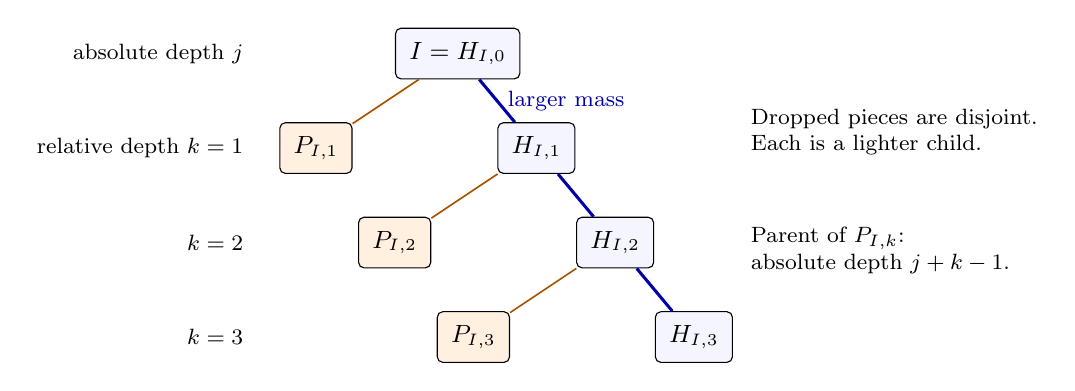
\begin{tikzpicture}[
  interval/.style={draw,rounded corners=2pt,inner sep=5pt,
                   fill=blue!4,font=\small},
  lighter/.style={draw,rounded corners=2pt,inner sep=5pt,
                  fill=orange!12,font=\small},
  heavyedge/.style={line width=1.1pt,blue!65!black},
  lightedge/.style={line width=.6pt,orange!65!black},
  note/.style={font=\footnotesize,align=left}
]
\node[interval] (root) at (0,0) {$I=H_{I,0}$};
\node[lighter] (p1) at (-1.8,-1.2) {$P_{I,1}$};
\node[interval] (h1) at (1.0,-1.2) {$H_{I,1}$};
\node[lighter] (p2) at (-.8,-2.4) {$P_{I,2}$};
\node[interval] (h2) at (2.0,-2.4) {$H_{I,2}$};
\node[lighter] (p3) at (.2,-3.6) {$P_{I,3}$};
\node[interval] (h3) at (3.0,-3.6) {$H_{I,3}$};
\draw[lightedge] (root)--(p1);
\draw[heavyedge] (root)--node[right,note] {larger mass}(h1);
\draw[lightedge] (h1)--(p2);
\draw[heavyedge] (h1)--(h2);
\draw[lightedge] (h2)--(p3);
\draw[heavyedge] (h2)--(h3);
\node[note,anchor=east] at (-2.6,0) {absolute depth $j$};
\node[note,anchor=east] at (-2.6,-1.2) {relative depth $k=1$};
\node[note,anchor=east] at (-2.6,-2.4) {$k=2$};
\node[note,anchor=east] at (-2.6,-3.6) {$k=3$};
\node[note,anchor=west] at (3.6,-1.0)
  {Dropped pieces are disjoint.\\
   Each is a lighter child.};
\node[note,anchor=west] at (3.6,-2.5)
  {Parent of $P_{I,k}$:\\
   absolute depth $j+k-1$.};
\end{tikzpicture}
\caption{Three steps of the heavier-child path.  At each step the
 lighter sibling is set aside; the chosen child is split again.  The
 dropped siblings together with the terminal child partition $I$.
 For fixed relative depth $k$, changing the frequency index $j$ changes
 the absolute depth of the parent.  This makes the parents distinct in
 the sum controlled by the convexity deficit.}
\label{fig:endpoint-tree}
\end{figure}


By additivity of $G_N$ and the triangle inequality in frequency $L^2$,
followed by \eqref{eq:endpoint-interpolated-dual},
\[
 e_j(I)^{1/2}
 \le C\sum_{k=1}^j2^{-k/6}m_{P_{I,k}}^{\alpha/2}
          +C2^{-j/6}m_{H_{I,j}}^{\alpha/2}.
\]
Use Cauchy--Schwarz with weights $2^{-k/6}$, including one additional
terminal weight $2^{-j/6}$.  Their sum is bounded independently of $j$.
Since $m_{H_{I,j}}\le m_I$, we obtain
\begin{equation}
 e_j(I)\le C\sum_{k=1}^j2^{-k/6}m_{P_{I,k}}^\alpha
                    +C2^{-j/6}m_I^\alpha.
 \label{eq:endpoint-heavy-path}
\end{equation}

We give the convexity calculation behind the sum of the first terms.
If a parent has child masses $a\ge b\ge0$, then
\begin{equation}
 (a+b)^\alpha-a^\alpha-b^\alpha
       \ge(2^\alpha-2)b^\alpha.
 \label{eq:endpoint-convexity-deficit}
\end{equation}
For $b>0$, divide by $b^\alpha$ and put $u=a/b\ge1$.
The function $(u+1)^\alpha-u^\alpha-1$ is increasing for $u\ge1$,
so its minimum is $2^\alpha-2$; the case $b=0$ is immediate.
Summing parent-minus-children deficits through depth $d-1$ telescopes to
\[
 m_{[0,1)}^\alpha-\sum_{Q\in\mathcal D_d}m_Q^\alpha
       \le m_{[0,1)}^\alpha.
\]
The deficits are nonnegative.  Letting $d\to\infty$ shows that the sum of
the lighter-child $\alpha$-powers over any collection of distinct dyadic
parents is at most
$m_{[0,1)}^\alpha/(2^\alpha-2)$.

Now fix $k\ge1$ and range over all $j\ge k$ and all
$I\in\mathcal D_j$.  The parent of $P_{I,k}$ is $H_{I,k-1}$, at absolute
depth $j+k-1$.  Different $j$ give different absolute depths; for the
same $j$, different $I$ have disjoint descendants.  These parents are
therefore distinct.  Consequently,
\[
 \sum_{j\ge k}\sum_{I\in\mathcal D_j}m_{P_{I,k}}^\alpha
      \le \frac{m_{[0,1)}^\alpha}{2^\alpha-2}.
\]
For the terminal terms, superadditivity of the $\alpha$th power gives
$\sum_{I\in\mathcal D_j}m_I^\alpha\le m_{[0,1)}^\alpha$.  Thus summing
\eqref{eq:endpoint-heavy-path}, first at fixed $k$ and then in $k$, gives
\[
 \sum_{j\ge1}\sum_{I\in\mathcal D_j}e_j(I)
 \le C m_{[0,1)}^\alpha
       \left(\sum_{k\ge1}2^{-k/6}+\sum_{j\ge1}2^{-j/6}\right)
 \le C.
\]
All sums are of nonnegative terms, so these rearrangements also follow
from finite truncations.  Finally apply
Lemma~\ref{lem:endpoint-time-separation} and sum its $O(2^{-2j})$ errors.
\end{proof}

\begin{remark}
The strict inequality $p>2$ is used quantitatively here:
$\alpha=3/2-1/p>1$ and $2^\alpha-2>0$.  At $p=2$ the convexity deficit
in \eqref{eq:endpoint-convexity-deficit} vanishes.  The gain in the time
tree therefore cannot be recovered merely from a weak $L^2$ version of
\eqref{eq:src24}.
\end{remark}

\begin{theorem}[Local strong maximal estimate]
\label{thm:maximal}
There is a constant $C$ such that, for every $f\in H^{1/3}(\R^2)$ whose
Fourier transform has compact support and every $x_0\in\R^2$,
\begin{equation}
 \int_{B(x_0,1)}\sup_{0\le t<1}|S(t)f(x)|\,dx
       \le C\|f\|_{H^{1/3}}.
 \label{eq:endpoint-strong-maximal}
\end{equation}
For arbitrary $f\in H^{1/3}(\R^2)$ there is a jointly measurable
representative $v_f(x,t)$, $0\le t<1$, continuous in $t$ for almost every
$x$, equal to $S(t)f$ as an $L^2$ function for each fixed $t$, and satisfying
the same bound with $S(t)f(x)$ replaced by $v_f(x,t)$.
\end{theorem}

\begin{proof}
First suppose $\widehat f$ has compact support.  Take a smooth frequency
partition
\[
 \psi_0+\sum_{j\ge1}\psi_j=1,
\]
where $\psi_0$ is supported in a fixed ball and $\psi_j$ is supported on
an annulus $|\xi|\asymp2^j$, with uniformly bounded overlap.  Put
$\widehat f_j=\psi_j\widehat f$.  Choose enlarged smooth annular cutoffs
$\chi_{2^j}$ equal to one on $\supp\psi_j$.  These are the cutoffs used in
Lemma~\ref{lem:endpoint-square-sum}.

For any common graph $t(x)$ and phase $w(x)$, Fourier inversion and the
definition of $G_N$ give
\[
 \int_\Omega w(x)\sum_{j\ge1}S(t(x))f_j(x)\,dx
       =(2\pi)^{-2}\sum_{j\ge1}
             \int\widehat f_j(\xi)G_{2^j}([0,1))(\xi)\,d\xi.
\]
Only finitely many summands are nonzero.  Cauchy--Schwarz in frequency
and in $j$ bounds the modulus by
\begin{align}
 C\left(\sum_{j\ge1}2^{2j/3}\|\widehat f_j\|_2^2\right)^{1/2}
  \left(\sum_{j\ge1}2^{-2j/3}
              \|G_{2^j}([0,1))\|_2^2\right)^{1/2}
 &\le C\|f\|_{H^{1/3}}.
 \label{eq:endpoint-frequency-cauchy-schwarz}
\end{align}
The first factor is bounded by the Sobolev square norm because on the
support of $\psi_j$ one has
$2^{2j/3}\asymp(1+|\xi|^2)^{1/3}$, and the supports overlap boundedly.
The second factor is bounded by \eqref{eq:endpoint-square-sum}.
The low-frequency term satisfies
$\sup_{x,t}|S(t)f_0(x)|\le C\|f_0\|_2$ by Cauchy--Schwarz on its fixed
frequency ball, so its integral over $\Omega$ has the same bound.

To recover the maximal function, take any finite list of times in
$[0,1)$ and let $t(x)$ be the first time attaining the maximal modulus
of $S(t)f(x)$ on that list.  Set
$w(x)=\overline{S(t(x))f(x)}/|S(t(x))f(x)|$ where the denominator is
nonzero, and set $w(x)=0$ otherwise.  These are measurable choices, and
the linearized integral is exactly the integral of the finite maximum.
Increase the list to a countable dense subset of $[0,1)$ containing zero.
Continuity in time and monotone convergence prove
\eqref{eq:endpoint-strong-maximal}.  The estimates above used only fixed
ball radii and spatial differences, so the constant is uniform in $x_0$.

For general $f$, choose $f_n$ with $\widehat f_n\in C_c^\infty(\R^2)$
and $\|f_n-f\|_{H^{1/3}}\le2^{-n}$.  In particular,
\[
 \sum_{n\ge1}\|f_{n+1}-f_n\|_{H^{1/3}}<\infty.
\]
Define the measurable functions
\[
 d_n(x)=\sup_{0\le t<1}
              |S(t)f_{n+1}(x)-S(t)f_n(x)|.
\]
The supremum can be taken over rational times, together with zero.
By \eqref{eq:endpoint-strong-maximal},
\[
 \sup_{x_0\in\R^2}\int_{B(x_0,1)}\sum_{n\ge1}d_n(x)\,dx
 \le C\sum_{n\ge1}\|f_{n+1}-f_n\|_{H^{1/3}}<\infty.
\]
A countable covering of $\R^2$ by unit balls therefore gives a single
full-measure set $E_0$ on which $\sum_n d_n(x)<\infty$.  For each
$x\in E_0$ the sequence $S(t)f_n(x)$ converges uniformly over
$0\le t<1$.  Denote its limit by $v_f(x,t)$, and define $v_f(x,t)=0$ for
$x\notin E_0$.  It is jointly measurable, and its time dependence is
continuous at every point of $E_0$, as a uniform limit of continuous
functions.

For each fixed $t$, unitarity gives $S(t)f_n\to S(t)f$ in $L^2$.
The pointwise limit on $E_0$ must therefore agree almost everywhere with
that $L^2$ limit.  This identifies the $L^2$ class of $v_f(\cdot,t)$ for
every fixed $t$; it does not assert a pointwise intersection over
uncountably many times.  Finally, Fatou's lemma in the maximal estimate
gives
\[
 \int_{B(x_0,1)}\sup_{0\le t<1}|v_f(x,t)|\,dx
    \le C\lim_{n\to\infty}\|f_n\|_{H^{1/3}}
    =C\|f\|_{H^{1/3}}.
\]
\end{proof}

\subsection{Recovering the Gaussian-first, all-real-time limit}

Fix $f\in H^{1/3}(\R^2)$ and the approximants just constructed, and write
$v=v_f$.  The same argument gives error envelopes with both pointwise
decay and spatial control at infinity.  Namely, let
\begin{equation}
 M_n(x)=\sup_{0\le t<1}|v(x,t)-S(t)f_n(x)|.
 \label{eq:endpoint-error-envelope}
\end{equation}
These functions are measurable by the rational-time supremum, since
the chosen $v(x,\cdot)$ is continuous even on the complement where it was
defined to be zero.  On $E_0$ the convergence is uniform, so
$M_n(x)\to0$.  Applying \eqref{eq:endpoint-strong-maximal} to
$f_\ell-f_n$ and then using Fatou yields
\begin{equation}
 \sup_{x_0\in\R^2}\int_{B(x_0,1)}M_n(x)\,dx
       \le C\|f-f_n\|_{H^{1/3}}.
 \label{eq:endpoint-envelope-local-mass}
\end{equation}
In particular, every $M_n$ is locally integrable with uniformly bounded
integrals over all translated unit balls.  This uniformity controls
Gaussian convolution far from its evaluation point.

\begin{lemma}[Gaussian approximation with uniform local mass]
\label{lem:endpoint-heat-envelope}
Let $h\ge0$ be locally integrable on $\R^2$ and suppose
\[
 A=\sup_{z\in\R^2}\int_{B(z,1)}h(y)\,dy<\infty.
\]
For $a>0$ let
\[
 K_a(z)=\frac1{4\pi a}e^{-|z|^2/(4a)}.
\]
Then $(K_a*h)(x)$ is finite for every $a>0$ and every $x$.  At every
Lebesgue point $x$ of $h$,
\begin{equation}
 \lim_{a\downarrow0}(K_a*h)(x)=h(x).
 \label{eq:endpoint-heat-envelope-limit}
\end{equation}
\end{lemma}

\begin{proof}
For a fixed $\rho>0$, cover each annulus
$2^\ell\rho\le |z|<2^{\ell+1}\rho$ by at most
$C(1+2^\ell\rho)^2$ unit balls.  Positivity gives
\begin{align}
 \int_{|z|\ge\rho}K_a(z)h(x-z)\,dz
 &\le \frac{CA}{a}\sum_{\ell\ge0}(1+2^\ell\rho)^2
                       e^{-4^\ell\rho^2/(4a)}\notag\\
 &\le C_\rho A a^{-1}e^{-\rho^2/(8a)},
 \qquad 0<a\le\min\{1,\rho^2\}.
 \label{eq:endpoint-gaussian-tail}
\end{align}
The series in the first line is finite for every fixed $a>0$.  Together
with local integrability this proves finiteness of the convolution, and
the second line shows that its distant contribution tends to zero.

At a Lebesgue point $x$, put
$H_x(r)=\int_{|z|<r}|h(x-z)-h(x)|\,dz=o(r^2)$.
Given $\varepsilon>0$, choose $\rho>0$ so that
$H_x(r)\le\varepsilon r^2$ for $0<r\le\rho$.  With
$k_a(r)=(4\pi a)^{-1}e^{-r^2/(4a)}$, radial integration by parts gives
\begin{align*}
 \int_{|z|<\rho}K_a(z)|h(x-z)-h(x)|\,dz
 &=k_a(\rho)H_x(\rho)
       +\int_0^\rho(-k_a'(r))H_x(r)\,dr\\
 &\le\varepsilon\left(k_a(\rho)\rho^2
                  +\int_0^\rho(-k_a'(r))r^2\,dr\right)
 \le C\varepsilon.
\end{align*}
Outside this neighborhood, \eqref{eq:endpoint-gaussian-tail} controls
the $h$ term, and the constant $h(x)$ is controlled by the vanishing
Gaussian mass outside $B(0,\rho)$.  Let $a\downarrow0$ and then
$\varepsilon\downarrow0$.
\end{proof}

\begin{proof}[Proof of Theorem~\ref{thm:main}]
At time zero, the fixed-time $L^2$ identification in
Theorem~\ref{thm:maximal} gives $v(\cdot,0)=f$ in $L^2$.  Since $f^*$
represents the same $L^2$ function on the set of Lebesgue points of $f$,
intersect $E_0$ with the full-measure set where $v(x,0)=f^*(x)$ and
with that Lebesgue-point set.
Next intersect with the Lebesgue-point sets of the countably many
functions $M_n$.  Call the resulting full-measure set $E$.  For every
$x\in E$ we now have, simultaneously,
\begin{equation}
 \begin{gathered}
 v(x,\cdot)\text{ is continuous on }[0,1),\qquad v(x,0)=f^*(x),\\
 M_n(x)\longrightarrow0,\qquad
 (K_a*M_n)(x)\longrightarrow M_n(x)
       \quad\text{as }a\downarrow0\text{ for every }n.
 \end{gathered}
 \label{eq:endpoint-common-good-set}
\end{equation}
The last assertion follows from
\eqref{eq:endpoint-envelope-local-mass} and
Lemma~\ref{lem:endpoint-heat-envelope}.  Only countably many exceptional
sets were removed.

For each fixed $t\in[0,1)$, the function $v(\cdot,t)$ represents
$S(t)f$ in $L^2$.  Since $K_a(x-\cdot)\in L^2$, convolution at a given
$x$ is an $L^2$ pairing and is independent of the representative of this
$L^2$ class.  Plancherel's identity therefore gives
\begin{equation}
 (K_a*v(\cdot,t))(x)
  =\frac1{(2\pi)^2}\int e^{ix\cdot\xi-it|\xi|^2-a|\xi|^2}
                                \widehat f(\xi)\,d\xi
  =U_af(x,t)
 \label{eq:endpoint-exact-convolution}
\end{equation}
for every $x\in\R^2$, every $a>0$, and every $0<t<1$.
The integral is absolutely convergent by Cauchy--Schwarz.  The
quantifiers in this step are significant: for each arbitrary $t$, an
identity of $L^2$ classes gives the convolution identity at every
evaluation point.  There is no intersection of time-dependent pointwise
exceptional sets in \eqref{eq:endpoint-exact-convolution}.

For the approximants, absolute Fourier integrability yields
\begin{align}
 R_n(a)&:=\sup_{x\in\R^2,\,0<t<1}
               |U_af_n(x,t)-S(t)f_n(x)|\notag\\
 &\le\frac1{(2\pi)^2}\int
               |1-e^{-a|\xi|^2}|\,|\widehat f_n(\xi)|\,d\xi
       \longrightarrow0\qquad(a\downarrow0).
 \label{eq:endpoint-smooth-heat-limit}
\end{align}
Positivity of $K_a$, the error envelope, and
\eqref{eq:endpoint-exact-convolution} give, for each $x\in E$,
\begin{equation}
 \sup_{0<t<1}|U_af(x,t)-v(x,t)|
 \le (K_a*M_n)(x)+M_n(x)+R_n(a).
 \label{eq:endpoint-uniform-gaussian-comparison}
\end{equation}
Indeed the difference between the two convolutions is bounded by
$K_a*M_n$, because
$|v(y,t)-S(t)f_n(y)|\le M_n(y)$ for almost every $y$, simultaneously for
all $t$; the remaining two differences are bounded by $R_n(a)$ and
$M_n(x)$.  All these convolutions are finite by the preceding lemma or
by the $L^2$ pairing.

Fix $n$ and take $\limsup_{a\downarrow0}$ in
\eqref{eq:endpoint-uniform-gaussian-comparison}.  By
\eqref{eq:endpoint-common-good-set} and
\eqref{eq:endpoint-smooth-heat-limit},
\[
 \limsup_{a\downarrow0}\sup_{0<t<1}|U_af(x,t)-v(x,t)|
        \le2M_n(x).
\]
Let $n\to\infty$.  Thus for every $x\in E$,
\begin{equation}
 \lim_{a\downarrow0}\sup_{0<t<1}|U_af(x,t)-v(x,t)|=0.
 \label{eq:endpoint-uniform-gaussian-limit}
\end{equation}
In particular, at each such $x$ the finite limit defining $u_f(x,t)$
exists for every real $0<t<1$, with $t$ fixed before $a$ tends to zero,
and it equals $v(x,t)$.  Continuity at zero now gives
\[
 \lim_{\substack{t\downarrow0\\t\in\R}}u_f(x,t)
     =\lim_{t\downarrow0}v(x,t)=v(x,0)=f^*(x).
\]
This proves Theorem~\ref{thm:main}.
\end{proof}

\clearpage
\phantomsection
\addcontentsline{toc}{section}{References}
\begin{thebibliography}{99}

\bibitem{BCT06}
J.~Bennett, A.~Carbery, and T.~Tao,
\emph{On the multilinear restriction and Kakeya conjectures},
Acta Math. \textbf{196} (2006), no.~2, 261--302.
\href{https://doi.org/10.1007/s11511-006-0006-4}{doi:10.1007/s11511-006-0006-4}.
\href{https://arxiv.org/abs/math/0509262v1}{arXiv:math/0509262v1}.

\bibitem{Bourgain95}
J.~Bourgain,
\emph{Some new estimates on oscillatory integrals},
in \emph{Essays on Fourier Analysis in Honor of Elias M.~Stein}
(C.~Fefferman, R.~Fefferman, and S.~Wainger, eds.),
Princeton Math. Ser., vol.~42,
Princeton Univ. Press, 1995, pp.~83--112.
\href{https://repo-archives.ihes.fr/FONDS_IHES/I_Prepublications/BOURGAIN/1990-1995/M_91_60/M_91_60_web.pdf}{Author preprint}.

\bibitem{Bourgain13}
J.~Bourgain,
\emph{On the Schr\"odinger maximal function in higher dimension},
Proc. Steklov Inst. Math. \textbf{280} (2013), 46--60.
\href{https://doi.org/10.1134/S0081543813010045}{doi:10.1134/S0081543813010045}.
\href{https://arxiv.org/abs/1201.3342}{arXiv:1201.3342}.

\bibitem{Bourgain16}
J.~Bourgain,
\emph{A note on the Schr\"odinger maximal function},
J. Anal. Math. \textbf{130} (2016), 393--396.
\href{https://doi.org/10.1007/s11854-016-0042-8}{doi:10.1007/s11854-016-0042-8}.
\href{https://arxiv.org/abs/1609.05744}{arXiv:1609.05744}.

\bibitem{BD15}
J.~Bourgain and C.~Demeter,
\emph{The proof of the $l^2$ Decoupling Conjecture},
Ann. of Math. (2) \textbf{182} (2015), no.~1, 351--389.
\href{https://doi.org/10.4007/annals.2015.182.1.9}{doi:10.4007/annals.2015.182.1.9}.
\href{https://arxiv.org/abs/1403.5335v3}{arXiv:1403.5335v3}.

\bibitem{BG11}
J.~Bourgain and L.~Guth,
\emph{Bounds on oscillatory integral operators based on multilinear estimates},
Geom. Funct. Anal. \textbf{21} (2011), no.~6, 1239--1295.
\href{https://doi.org/10.1007/s00039-011-0140-9}{doi:10.1007/s00039-011-0140-9}.
\href{https://arxiv.org/abs/1012.3760}{arXiv:1012.3760}.

\bibitem{Carleson80}
L.~Carleson,
\emph{Some analytic problems related to statistical mechanics},
in \emph{Euclidean Harmonic Analysis}
(J.~J.~Benedetto, ed.),
Lecture Notes in Math., vol.~779,
Springer, Berlin, 1980, pp.~5--45.
\href{https://doi.org/10.1007/BFb0087666}{doi:10.1007/BFb0087666}.

\bibitem{CK01}
M.~Christ and A.~Kiselev,
\emph{Maximal functions associated to filtrations},
J. Funct. Anal. \textbf{179} (2001), no.~2, 409--425.
\href{https://doi.org/10.1006/jfan.2000.3687}{doi:10.1006/jfan.2000.3687}.

\bibitem{DahlbergKenig82}
B.~E.~J.~Dahlberg and C.~E.~Kenig,
\emph{A note on the almost everywhere behavior of solutions to the
Schr\"odinger equation},
in \emph{Harmonic Analysis}
(F.~Ricci and G.~Weiss, eds.),
Lecture Notes in Math., vol.~908,
Springer, Berlin, 1982, pp.~205--209.
\href{https://doi.org/10.1007/BFb0093289}{doi:10.1007/BFb0093289}.

\bibitem{DFGGL26}
Y.~Deng, C.~Fan, S.~Guo, Z.~Guo, and Y.~Luo,
\emph{Sharp Strichartz estimates on the one-dimensional torus},
arXiv:2609.18670v1 (2026).
\href{https://arxiv.org/abs/2609.18670v1}{arXiv:2609.18670v1}.

\bibitem{DGL17}
X.~Du, L.~Guth, and X.~Li,
\emph{A sharp Schr\"odinger maximal estimate in $\mathbb R^2$},
Ann. of Math. (2) \textbf{186} (2017), no.~2, 607--640.
\href{https://doi.org/10.4007/annals.2017.186.2.5}{doi:10.4007/annals.2017.186.2.5}.

\bibitem{DGLZ18}
X.~Du, L.~Guth, X.~Li, and R.~Zhang,
\emph{Pointwise convergence of Schr\"odinger solutions and multilinear refined
Strichartz estimates},
Forum Math. Sigma \textbf{6} (2018), e14, 18 pp.
\href{https://doi.org/10.1017/fms.2018.11}{doi:10.1017/fms.2018.11}.
\href{https://arxiv.org/abs/1803.01720v2}{arXiv:1803.01720v2}.

\bibitem{DZ19}
X.~Du and R.~Zhang,
\emph{Sharp $L^2$ estimates of the Schr\"odinger maximal function
in higher dimensions},
Ann. of Math. (2) \textbf{189} (2019), no.~3, 837--861.
\href{https://doi.org/10.4007/annals.2019.189.3.4}{doi:10.4007/annals.2019.189.3.4}.
\href{https://arxiv.org/abs/1805.02775v3}{arXiv:1805.02775v3}.

\bibitem{GLY23}
S.~Guo, Z.~K.~Li, and P.-L.~Yung,
\emph{Improved discrete restriction for the parabola},
Math. Res. Lett. \textbf{30} (2023), no.~5, 1375--1409.
\href{https://arxiv.org/abs/2103.09795v2}{arXiv:2103.09795v2}.

\bibitem{GK15}
L.~Guth and N.~H.~Katz,
\emph{On the Erd\H{o}s distinct distances problem in the plane},
Ann. of Math. (2) \textbf{181} (2015), no.~1, 155--190.
\href{https://doi.org/10.4007/annals.2015.181.1.2}{doi:10.4007/annals.2015.181.1.2}.
\href{https://arxiv.org/abs/1011.4105v3}{arXiv:1011.4105v3}.

\bibitem{GMW24}
L.~Guth, D.~Maldague, and H.~Wang,
\emph{Improved decoupling for the parabola},
J. Eur. Math. Soc. (JEMS) \textbf{26} (2024), no.~3, 875--917.
\href{https://doi.org/10.4171/JEMS/1295}{doi:10.4171/JEMS/1295}.
\href{https://arxiv.org/abs/2009.07953}{arXiv:2009.07953}.

\bibitem{He20}
W.~He,
\emph{Orthogonal projections of discretized sets},
J. Fractal Geom. \textbf{7} (2020), no.~3, 271--317.
\href{https://doi.org/10.4171/JFG/92}{doi:10.4171/JFG/92}.
\href{https://arxiv.org/abs/1710.00795v2}{arXiv:1710.00795v2}.

\bibitem{Lee06}
S.~Lee,
\emph{On pointwise convergence of the solutions to Schr\"odinger equations
in $\mathbb R^2$},
Int. Math. Res. Not. (2006), Art.~ID 32597, 21 pp.
\href{https://doi.org/10.1155/IMRN/2006/32597}{doi:10.1155/IMRN/2006/32597}.

\bibitem{LiYung26}
Z.~K.~Li and P.-L.~Yung,
\emph{An improved high-low method for the parabola},\newline
\href{https://arxiv.org/abs/2609.33949v1}{arXiv:2609.33949v1} (2026).

\bibitem{MVV96}
A.~Moyua, A.~Vargas, and L.~Vega,
\emph{Schr\"odinger maximal function and restriction properties of the
Fourier transform},
Int. Math. Res. Not. \textbf{1996} (1996), no.~16, 793--815.
\href{https://doi.org/10.1155/S1073792896000499}{doi:10.1155/S1073792896000499}.

\bibitem{PanSunTan26}
Y.~Pan, W.~Sun, and J.~Tan,
\emph{Pointwise convergence of Schr\"odinger operators in Bessel potential
spaces},
arXiv:2605.25833v2 (2026).
\href{https://arxiv.org/abs/2605.25833v2}{arXiv:2605.25833v2}.

\bibitem{SjogrenSjolin89}
P.~Sj\"ogren and P.~Sj\"olin,
\emph{Convergence properties for the time-dependent Schr\"odinger equation},
Ann. Acad. Sci. Fenn. Ser. A I Math. \textbf{14} (1989), 13--25.
\href{https://www.acadsci.fi/mathematica/Vol14/vol14pp013-025.pdf}{Journal PDF}.

\bibitem{Sjolin87}
P.~Sj\"olin,
\emph{Regularity of solutions to the Schr\"odinger equation},
Duke Math. J. \textbf{55} (1987), no.~3, 699--715.
\href{https://doi.org/10.1215/S0012-7094-87-05535-9}{doi:10.1215/S0012-7094-87-05535-9}.

\bibitem{Tao03}
T.~Tao,
\emph{A sharp bilinear restriction estimate for paraboloids},
Geom. Funct. Anal. \textbf{13} (2003), no.~6, 1359--1384.
\href{https://doi.org/10.1007/s00039-003-0449-0}{doi:10.1007/s00039-003-0449-0}.
\href{https://arxiv.org/abs/math/0210084}{arXiv:math/0210084}.

\bibitem{TV00}
T.~Tao and A.~Vargas,
\emph{A bilinear approach to cone multipliers. II. Applications},
Geom. Funct. Anal. \textbf{10} (2000), no.~1, 216--258.
\href{https://doi.org/10.1007/s000390050007}{doi:10.1007/s000390050007}.

\bibitem{Vega88}
L.~Vega,
\emph{Schr\"odinger equations: pointwise convergence to the initial data},
Proc. Amer. Math. Soc. \textbf{102} (1988), no.~4, 874--878.
\href{https://doi.org/10.1090/S0002-9939-1988-0934859-0}{doi:10.1090/S0002-9939-1988-0934859-0}.

\bibitem{W93}
R.~Wongkew,
\emph{Volumes of tubular neighbourhoods of real algebraic varieties},
Pacific J. Math. \textbf{159} (1993), no.~1, 177--184.
\href{https://doi.org/10.2140/pjm.1993.159.177}{doi:10.2140/pjm.1993.159.177}.

\end{thebibliography}

\end{document}
